% ==============================================================================
% فایل اصلی پایان‌نامه کارشناسی (Master Thesis File)
% دانشگاه تهران - دانشکدگان فنی - دانشکده مهندسی برق و کامپیوتر
% عنوان: طراحی سیستم تأمین داده جهت استنتاج WCET
% نگارش: محمد مهدی دوست محمدی (810100142)
% استاد راهنما: دکتر مهدی کارگهی
% ==============================================================================

\documentclass[12pt,a4paper,oneside]{book}

% فراخوانی تنظیمات، بسته‌ها و استایل‌ها
% ==============================================================================
% فایل تنظیمات و بسته‌های نگارش پایان‌نامه (Preamble)
% دانشگاه تهران - دانشکدگان فنی - دانشکده مهندسی برق و کامپیوتر
% طراحی سیستم تأمین داده جهت استنتاج WCET
% دانشجو: محمد مهدی دوست محمدی (810100142)
% ==============================================================================

% تنظیمات ابعاد صفحه و حاشیه‌ها (مطابق فایل الگوی گزارش PSA1 و دانشگاه تهران)
\usepackage[
    a4paper,
    top=30mm,
    bottom=25.4mm,
    left=22.2mm,
    right=24.3mm,
    headheight=16pt,
    footskip=12mm
]{geometry}

% تنظیم عمق فهرست مطالب و شماره‌گذاری بخش‌ها (تنها فصول، بخش‌ها و زیربخش‌ها)
\setcounter{secnumdepth}{2}
\setcounter{tocdepth}{2}

% بسته‌های ریاضی و نمادها
\usepackage{amsmath}
\usepackage{amssymb}
\usepackage{amsfonts}
\usepackage{mathtools}

% بسته‌های درج تصاویر، نمودارها و رنگ‌ها
\usepackage{graphicx}
\usepackage{xcolor}
\usepackage{tikz}
\usetikzlibrary{shapes.geometric, arrows.meta, positioning, calc, fit, backgrounds}
\usepackage{eso-pic}

% بسته‌های جداول پیشرفته
\usepackage{booktabs}
\usepackage{tabularx}
\usepackage{multirow}
\usepackage{array}
\usepackage{float}
\usepackage{caption}
\usepackage{subcaption}

% بسته‌های نمایش کد و الگوریتم
\usepackage{listings}
\usepackage{tcolorbox}
\tcbuselibrary{skins, breakable}

% تنظیمات سربرگ و پانویس (Header & Footer)
\usepackage{fancyhdr}
\pagestyle{fancy}
\fancyhf{}
\fancyhead[R]{\small\slshape \leftmark}
\fancyhead[L]{\small\thepage}
\fancyfoot[C]{}
\renewcommand{\headrulewidth}{0.6pt}
\renewcommand{\footrulewidth}{0pt}

% استایل صفحات ابتدایی فصل‌ها
\fancypagestyle{plain}{
    \fancyhf{}
    \fancyfoot[C]{\small\thepage}
    \renewcommand{\headrulewidth}{0pt}
}

% تعریف کادربندی ظریف دور صفحه (مطابق با کادربندی موجود در PSA1_FP_Report)
\AddToShipoutPictureBG{%
  \begin{tikzpicture}[remember picture, overlay]
    \draw[line width=0.6pt, color=gray!80]
      ($(current page.north west) + (1.2cm, -1.2cm)$)
      rectangle
      ($(current page.south east) + (-1.2cm, 1.2cm)$);
  \end{tikzpicture}%
}

% تنظیمات لینک‌ها و بوکمارک‌های پی‌دی‌اف
\usepackage{hyperref}
\hypersetup{
    pdfpagelabels=false,
    colorlinks=true,
    linkcolor=blue!75!black,
    citecolor=green!60!black,
    urlcolor=blue!85!black,
    filecolor=magenta,
    pdfstartview={FitH},
    pdfauthor={محمد مهدی دوست محمدی},
    pdftitle={طراحی سیستم تأمین داده جهت استنتاج WCET},
    pdfsubject={پایان‌نامه کارشناسی مهندسی برق - الکترونیک},
    pdfkeywords={WCET, ARM Cortex-M7, ETM, CoreSight, OpenCSD, STM32H7, Instruction Trace}
}

% تنظیمات نمایش کدهای برنامه‌نویسی (C, Python, Assembly)
\definecolor{codegreen}{rgb}{0,0.6,0}
\definecolor{codegray}{rgb}{0.5,0.5,0.5}
\definecolor{codepurple}{rgb}{0.58,0,0.82}
\definecolor{backcolour}{rgb}{0.97,0.97,0.97}

\lstdefinestyle{customc}{
    backgroundcolor=\color{backcolour},
    commentstyle=\color{codegreen},
    keywordstyle=\color{blue}\bfseries,
    numberstyle=\tiny\color{codegray},
    stringstyle=\color{codepurple},
    basicstyle=\ttfamily\footnotesize,
    breakatwhitespace=false,
    breaklines=true,
    captionpos=b,
    keepspaces=true,
    numbers=left,
    numbersep=5pt,
    showspaces=false,
    showstringspaces=false,
    showtabs=false,
    tabsize=2,
    frame=single,
    rulecolor=\color{black!20}
}
\lstset{style=customc}

% سازگاری کرنل جدید لاتک با ماژول‌های bidi در TeX Live 2026
\providecommand{\UseMathForPositioningText}{}
\providecommand{\UseTaggingSocket}[1]{}

% نادیده‌گرفتن نویسه نامرئی U+200F جهت سازگاری با فونت‌های تک‌فاصله
\usepackage{newunicodechar}
\newunicodechar{‏}{}

% ------------------------------------------------------------------------------
% بسته زی‌پرشین (باید همواره آخرین بسته فراخوانی‌شده باشد)
% ------------------------------------------------------------------------------
\usepackage{xepersian}

% تنظیم قلم‌های استاندارد زبان فارسی و انگلیسی (دو سایز بزرگتر و خواناتر)
\settextfont[
    Path=fonts/,
    BoldFont=BNaznnBd.ttf,
    Scale=1.22
]{BNazanin.ttf}
\setlatintextfont[Scale=1.1]{Times New Roman}

% تعریف قلم‌های سفارشی تیتر و عناوین
\defpersianfont\titr[
    Path=fonts/,
    Scale=1.28
]{BTitrBd.ttf}

\defpersianfont\zar[
    Path=fonts/,
    BoldFont=BZarBd.ttf,
    Scale=1.22
]{BZar.ttf}

% افزایش عمومی فاصله بین خطوط در سرتاسر متن پایان‌نامه
\linespread{1.35}

% ارقام فارسی در محیط‌های متنی و ریاضی
\SepMark{.}

% نمادهای بالت استاندارد با قلم ریاضی (جلوگیری از گلیف ناموجود در قلم متن فارسی)
\renewcommand{\labelitemi}{\ensuremath{\bullet}}
\renewcommand{\labelitemii}{\ensuremath{\circ}}
\renewcommand{\labelitemiii}{\ensuremath{\ast}}
\renewcommand{\labelitemiv}{\ensuremath{\cdot}}

% اصلاح عنوان مراجع برای جلوگیری از فونت ناموجود در سربرگ‌های لاتین
\renewcommand{\bibname}{مراجع}


\begin{document}

% ------------------------------------------------------------------------------
% بخش‌های ابتدایی (Front Matter)
% ------------------------------------------------------------------------------
\frontmatter

% روی جلد فارسی
% ==============================================================================
% صفحه روی جلد فارسی پایان‌نامه (Cover Page)
% ==============================================================================

\begin{titlepage}
\thispagestyle{empty}
\begin{center}

    % سربرگ رسمی: آرم دانشگاه تهران در راست، عناوین در مرکز، نشان دانشکدگان فنی در چپ
    \noindent
    \begin{minipage}[c]{0.22\textwidth}
        \begin{flushright}
            
\includegraphics[height=3.0cm]{figures/ut_logo.png}
        \end{flushright}
    \end{minipage}%
    \hfill
    \begin{minipage}[c]{0.52\textwidth}
        \centering
        {\bfseries\Large دانشگاه تهران}\\[0.25cm]
        {\bfseries\large دانشکدگان فنی}\\[0.25cm]
        {\bfseries\large دانشکده مهندسی برق و کامپیوتر}
    \end{minipage}%
    \hfill
    \begin{minipage}[c]{0.22\textwidth}
        \begin{flushleft}
            
\includegraphics[height=3.0cm]{figures/ut_emblem.jpg}
        \end{flushleft}
    \end{minipage}\\[0.8cm]

    {\large پایان‌نامه برای دریافت درجه کارشناسی}\\[0.25cm]
    {\large در رشته مهندسی برق، گرایش الکترونیک}\\[1.0cm]

    % عنوان پایان‌نامه با قلم تیتر بزرگ
    \begin{tcolorbox}[colback=white, colframe=gray!40!black, arc=3mm, width=0.95\textwidth, halign=center]
        \vspace{0.4cm}
        {\fontsize{24}{44}\selectfont\titr طراحی سیستم تأمین داده \\ جهت استنتاج \lr{WCET}\par}
        \vspace{0.4cm}
    \end{tcolorbox}

    \vspace{1.0cm}

    % مشخصات دانشجو و اساتید
    \begin{minipage}{0.85\textwidth}
        \large
        \textbf{نگارش:}\quad {\titr محمد مهدی دوست محمدی}\\[0.3cm]
        \textbf{شماره دانشجویی:}\quad 810100142\\[0.6cm]
        \textbf{استاد راهنما:}\quad {\titr دکتر مهدی کارگهی}\\[0.2cm]
        \small (دانشیار دانشکده مهندسی برق و کامپیوتر)\\[0.6cm]
        \textbf{محل انجام پروژه:}\quad دانشکده مهندسی برق و کامپیوتر دانشگاه تهران
    \end{minipage}

    \vfill

    % تاریخ
    {\large\bfseries شهریورماه ۱۴۰۵}

\end{center}
\end{titlepage}


% تعهدنامه اصالت اثر
% ==============================================================================
% تعهدنامه اصالت اثر
% ==============================================================================

\newpage
\thispagestyle{empty}

\begin{center}
    \vspace*{2cm}
    {\titr\Large تعهدنامه اصالت اثر}\\[1.5cm]
\end{center}

\noindent
اینجانب \textbf{محمد مهدی دوست محمدی} تائید می‌کنم که مطالب مندرج در این پایان‌نامه با عنوان:
\begin{center}
    \vspace{0.3cm}
    \textbf{«طراحی سیستم تأمین داده جهت استنتاج \lr{WCET}»}
    \vspace{0.3cm}
\end{center}
حاصل تلاش اینجانب است و به دستاوردهای پژوهشی دیگران که در این نوشته از آن‌ها استفاده شده است، مطابق مقررات علمی و دانشگاهی ارجاع گردیده است. این پایان‌نامه قبلاً برای احراز هیچ مدرک هم‌سطح یا بالاتر در هیچ دانشگاه یا مؤسسه‌ای ارائه نشده است.

\vspace{2cm}
\noindent
کلیه حقوق مادی و معنوی این اثر متعلق به دانشکدگان فنی دانشگاه تهران می‌باشد.

\vspace{2cm}

\begin{flushleft}
    \begin{minipage}{0.6\textwidth}
        \textbf{نام و نام خانوادگی دانشجو:}\quad محمد مهدی دوست محمدی\\[0.4cm]
        \textbf{شماره دانشجویی:}\quad 810100142\\[0.4cm]
        \textbf{امضای دانشجو:}\\[0.1cm]
        \hspace*{0.6cm}
\includegraphics[width=3.0cm]{figures/signature.png}\\[0.2cm]
        \textbf{تاریخ:}\quad شهریورماه ۱۴۰۵
    \end{minipage}
\end{flushleft}


% صفحه سپاسگزاری و تقدیم
% ==============================================================================
% سپاسگزاری و تقدیم
% ==============================================================================

\newpage
\thispagestyle{empty}

\begin{center}
    \vspace*{1cm}
    {\titr\Large سپاسگزاری و قدردانی}\\[1.2cm]
\end{center}

\noindent
در وهله نخست، مراتب سپاس و قدردانی صمیمانه و قلبی خود را تقدیم استاد راهنمای گرانقدرم، \textbf{دکتر مهدی کارگهی}، می‌نمایم. بدون تردید، راهنمایی‌های ارزشمند، نگاه ژرف علمی و حمایت‌های دلسوزانه ایشان در طول انجام این پروژه، چراغ راه و پشتیبان اصلی در عبور از چالش‌های پیچیده سخت‌افزاری و نرم‌افزاری این مسیر بود. از دانش بی‌پایان و اخلاق حرفه‌ای ایشان درس‌های فراوانی آموختم که همواره توشه راه پژوهشی و مهندسی‌ام خواهد بود.

\vspace{0.8cm}
\noindent
همچنین از دوست و همراه گرامی‌ام، \textbf{محمد حسن آملی}، که در پروژه مکمل استنتاج \lr{WCET} و طراحی سامانه تست خودکار همگام و پشتیبان بود و تبادل نظرات فنی با وی زمینه‌ساز غنای هر دو پروژه گردید، صمیمانه سپاسگزاری می‌کنم.

\vspace{0.8cm}
\noindent
در پایان، قدردان زحمات بی‌دریغ و حمایت‌های همیشگی \textbf{پدر و مادر عزیزم} هستم که آرامش، انگیزه و امکان ادامه این مسیر را با مهر بی‌کران خود برایم به ارمغان آوردند.


% شماره‌گذاری صفحات مقدماتی
\pagenumbering{tartibi}

% چکیده فارسی
% ==============================================================================
% چکیده فارسی
% ==============================================================================

\newpage
\thispagestyle{plain}

\begin{center}
    {\titr\Large چکیده}\\[1cm]
\end{center}

\noindent
در سامانه‌های تعبیه‌شده و بی‌درنگ سخت (\lr{Hard Real-Time Embedded Systems})، تخمین دقیق و تضمین‌پذیر بیشینه زمان اجرا (\lr{WCET}) عاملی حیاتی در اثبات ایمنی و زمان‌بندی‌پذیری سامانه به شمار می‌رود. در معماری‌های نوین پردازنده‌ها با خط‌لوله‌های چندمرحله‌ای، پیش‌بینی انشعاب و حافظه‌های نهان، روش‌های تحلیل ایستا به دلیل تخمین‌های بیش‌ازحد بدبینانه ناتوان بوده و در نقطه مقابل، رویکردهای سنتی ابزاردقیق نرم‌افزاری (\lr{Software Instrumentation}) با تحمیل سربار اجرایی و اعوجاج زمانی (پدیده «اثر پروب»)، رفتار اصیل پردازنده را دگرگون می‌سازند. این رساله به طراحی، پیاده‌سازی عملی و اعتبارسنجی جامع یک خط‌لوله غیرتهاجمی (\lr{Non-intrusive}) جهت تأمین داده‌های ردیابی اجرای برنامه و استنتاج دقیق \lr{WCET} در مقیاس چرخه ساعت پردازنده می‌پردازد.

سامانه ارائه‌شده با تمرکز بر ماژول ردیابی سخت‌افزاری \lr{ETMv4} در زیرساخت دیباگ \lr{ARM CoreSight} بر روی میکروکنترلر پیشرفته \lr{STM32H750 (ARM Cortex-M7)} توسعه یافته است. در این فرآیند، چالش‌های پیچیده پیکربندی ثبّاتی نظیر آزادسازی قفل‌های سخت‌افزاری، توزیع توان و کلاک و مغایرت‌های راهنمای مرجع تراشه با استاندارد معماری برطرف گردید. داده‌های فشرده ردیابی دستورات از طریق گذرگاه موازی ۴ بیتی درگاه \lr{TPIU} بدون تحمیل کوچک‌ترین سربار پردازشی صادر شده و توسط لاجیک‌آنالایزر دیجیتال با راهبرد اورسمپلینگ ۱۰ برابری ثبت می‌شوند. اسکریپت تخصصی \lr{\texttt{TraceStreamProcessor.py}} با ترازسازی فریم‌ها و جبران اعوجاج‌های فیزیکی، ساختار اسنپ‌شات استاندارد صنعتی را تولید کرده و با ادغام با موتور دکودر مرجع \lr{OpenCSD} و باینری \lr{ELF}، جریان تفکیک‌شده دستورات اسمبلی و برچسب‌های زمانی نانوثانیه‌ای را بازسازی می‌نماید. 

به منظور تبدیل این خط‌لوله به یک ابزار صنعتی و کاربرپسند، افزونه اختصاصی \lr{CoreSight Trace Studio} برای محیط توسعه \lr{VS Code} طراحی و پیاده‌سازی شد که در قالبی سه‌مرحله‌ای، متوالی و نیمه‌خودکار، فرآیند تزریق خودکار درایورها، نشانه‌گذاری پنجره‌های پایش در کدهای منبع، تولید متناظر مانیفست‌های اسنپ‌شات و نمایش لاگ‌های روند اجرای برنامه را در یک داشبورد مدرن محقق می‌سازد. در فاز ارزیابی تجربی، عملکرد سامانه تحت سناریوهای چالش‌برانگیز شامل آزمون دوره‌ای تایمر ۱۰۰ میکروثانیه با ثبت انحراف زمانی ناچیز زیر $0.1\ \mu\mathrm{s}$ (اثبات قطعی ماهیت غیرتهاجمی)، تطبیق زمانی سیگنال‌های فیزیکی، و رهگیری وقایع ترکیبی وقفه‌ها با هندشیک سخت‌افزاری به اثبات رسید. این بستر در هم‌افزایی با سامانه مکمل آزمون خودکار، پلتفرمی اقتصادی، بومی و کارا جهت آزمون برنامه‌های سیستم‌های نهفته و سنجش ایمنی آن‌ها به ارمغان آورده است. چه بسا این سیستم بتواند در آینده در قامت یک رقیب برای ابزارهای آزمون نرم‌افزار تجاری بین‌المللی واقع شود.

\vspace{1.0cm}
\noindent
\textbf{واژگان کلیدی:}\quad بیشینه زمان اجرا (\lr{WCET})، ردیابی غیرتهاجمی دستورات (\lr{Instruction Trace})، ماژول \lr{ETMv4}، معماری \lr{ARM CoreSight}، پردازنده \lr{Cortex-M7}، میکروکنترلر \lr{STM32H7}، دکودر \lr{OpenCSD}، افزونه \lr{CoreSight Trace Studio}، سامانه‌های بی‌درنگ سخت.


% فهرست مطالب
\newpage
\tableofcontents

% فهرست جداول
\newpage
\listoftables

% فهرست تصاویر و نمودارها
\newpage
\listoffigures

% ------------------------------------------------------------------------------
% متن اصلی پایان‌نامه (Main Matter)
% ------------------------------------------------------------------------------
\mainmatter
\pagenumbering{arabic}

% تقدم مراجع فنی، استانداردهای معماری و ابزارها بر مقالات آکادمیک در ترتیب فهرست منابع
\nocite{armcoresight2013,dslab2023dsview,armetmv42017,st2020stm32h7,linaroopencsd}

% فصل اول: کلیات، بیان مسئله و اهداف پروژه
% فصل اول: مقدمه و بیان مسئله
% ==============================================================================
% فصل اول: مقدمه و بیان مسئله
% ==============================================================================

\chapter{مقدمه و بیان مسئله}
\label{ch:intro}

\section{مقدمه و ضرورت پژوهش}
در دهه‌های اخیر، سامانه‌های تعبیه‌شده (\lr{Embedded Systems}) به ستون فقرات زیرساخت‌های حیاتی دنیای مدرن بدل شده‌اند؛ از سیستم‌های اویونیک و هدایت ناوبری در صنایع هوافضا و خودروهای هوشمند خودران گرفته تا تجهیزات کنترل علائم حیاتی در پزشکی و بازوهای رباتیک در خطوط اتوماسیون صنعتی. ویژگی مشترک و وجه تمایز بنیادین این رده از کاربردها، ماهیت «بی‌درنگ سخت» (\lr{Hard Real-Time}) آن‌ها است. در سامانه‌های بی‌درنگ سخت، درستی و صحت کل سامانه صرفاً به درستی محاسبات منطقی و ریاضی محدود نمی‌شود، بلکه عامل «زمان» به عنوان یک بُعد تعیین‌کننده و غیرقابل‌مذاکره وارد عمل می‌گردد. به بیان دقیق‌تر، تولید یک پاسخ کاملاً صحیح از نظر منطقی، چنانچه با حتی کسری از میلی‌ثانیه تأخیر پس از موعد مقرر (\lr{Deadline}) تحویل داده شود، در حکم خطای بحرانی سامانه بوده و می‌تواند فجایع جبران‌ناپذیر انسانی یا خسارات سنگین مالی به همراه داشته باشد.

برای تحقق ضمانت‌های قطعی در زمان‌بندی‌پذیری (\lr{Schedulability})، مهندسان سیستم‌های بی‌درنگ نیازمند دانستن کران بالای زمان اجرای تک‌تک وظایف محاسباتی هستند. این کران بیشینه، در متون علمی تحت عنوان «بیشینه زمان اجرا» (\lr{Worst-Case Execution Time - WCET}) شناخته می‌شود \cite{wilhelm2008worst}. استخراج دقیق و قابل‌اطمینان \lr{WCET} سنگ‌بنای طراحی سامانه‌های با قابلیت اطمینان بالا (\lr{High-Reliability}) و تخصیص منابع پردازشی است \cite{kargahi2008analytical}. با این وجود، به دلیل جهش‌های فنی گسترده در معماری پردازنده‌های تعبیه‌شده در سال‌های اخیر، محاسبه و استنتاج این کمیت به یکی از پیچیده‌ترین چالش‌های مهندسی الکترونیک و کامپیوتر مبدل گشته است.

در سطح صنایع پیشرفته جهانی، خودکارسازی فرآیند آزمون محصول و استنتاج غیرتهاجمی زمان‌بندی توسط پلتفرم‌های نرم‌افزاری انحصاری و بسیار پرهزینه نظیر سامانه‌های شرکت \lr{Rapita Systems} (مجموعه \lr{RVS / RapiTime})، بسترهای آزمون در حلقه سخت‌افزار (\lr{HIL}) شرکت \lr{Speedgoat} و ابزارهای مشابه انجام می‌پذیرد. هزینه لایسنس و به‌کارگیری این راهکارهای تجاری بالغ بر ده‌ها تا صدها هزار دلار (بیش از ۱۰ تا ۱۰۰ هزار دلار) بوده و دستیابی به آن‌ها نیازمند بودجه‌های سنگین است. از این رو، طراحی و توسعه یک پلتفرم جامع آزمون خودکار محصول و پایش غیرتهاجمی با حداقل هزینه ممکن، اهمیتی دوچندان و توجیه اقتصادی و کاربردی بسیار بالایی پیدا می‌کند.

\section{مسئله استنتاج \lr{WCET} و چالش‌های معماری پردازنده‌های مدرن}
در نسل‌های نخستین میکروکنترلرها (نظیر پردازنده‌های ۸ بیتی و ریزکنترلرهای اولیه)، خط سیر اجرای دستورات به شدت تعیینی (\lr{Deterministic}) بود؛ به طوری که هر دستورالعمل تعداد چرخه‌های کلاک مشخص و ثابتی را مصرف می‌کرد و طراح سیستم می‌توانست با جمع جبری زمان دستورات و بازرسی چشمی کد اسمبلی، بدترین زمان اجرای یک تابع را با دقت بالا تخمین بزند. اما در پردازنده‌های امروزی تعبیه‌شده با کارایی بالا (نظیر هسته‌های \lr{ARM Cortex-M7})، مجموعه‌ای از نوآوری‌های سخت‌افزاری جهت افزایش توان محاسباتی به کار گرفته شده است که رفتار زمانی پردازنده را به شدت پویا، غیرخطی و وابسته به کانتکست تاریخی اجرا می‌نماید:
\begin{enumerate}
    \item \textbf{خط‌لوله‌های چندمرحله‌ای و سوپراسکالر (\lr{Superscalar Pipelines}):} اجرای هم‌زمان بیش از یک دستور در چرخه کلاک و وابستگی‌های ساختاری داده‌ها (\lr{Data Hazards}).
    \item \textbf{حافظه‌های نهان چندسطحی (\lr{Instruction \& Data Caches}):} وابستگی زمان واکشی دستور به رخداد اصابت (\lr{Cache Hit}) یا عدم اصابت (\lr{Cache Miss})، که موجب نوسان زمان دسترسی از چند نانوثانیه تا ده‌ها چرخه کلاک می‌گردد.
    \item \textbf{واحدهای پیش‌بینی انشعاب (\lr{Branch Predictors}):} حدس زدن نتیجه شرط‌ها پیش از حل شدن آن‌ها و نیاز به پاک‌سازی خط‌لوله (\lr{Pipeline Flush}) در صورت پیش‌بینی نادرست.
    \item \textbf{تداخل گذرگاه‌ها و ساختارهای دسترسی مستقیم به حافظه (\lr{DMA}):} رقابت بر سر پهنای باند حافظه مشترک میان هسته و تجهیزات جانبی.
\end{enumerate}

این پدیده‌ها مجموعاً موجب بروز اثراتی موسوم به «ناهنجاری‌های زمانی» (\lr{Timing Anomalies}) می‌گردند؛ وضعیتی که در آن یک رخداد با فرض بهینه‌سازی محلی (مانند اصابت به حافظه نهان)، در مقیاس کلی به دلیل تغییر ترتیب تخصیص منابع منجر به تأخیر در اجرای کلی برنامه می‌شود \cite{cullmann2010predictability}. در چنین محیط‌های پویایی، استخراج کران بالای زمان اجرا صرفاً با استفاده از مدل‌های نظری ریاضی، یا به ارقام غیرواقعی و بیش‌ازحد محافظه‌کارانه (\lr{Over-conservative}) می‌انجامد که موجب اتلاف عظیم سخت‌افزار می‌شود، و یا به دلیل خطاهای تقریب مدل سخت‌افزاری، کران نامعتبری تولید می‌کند که نقض‌کننده ایمنی سامانه است.

\section{معضل ابزاردقیق نرم‌افزاری و پدیده «اثر پروب»}
برای رفع محدودیت‌های روش‌های صرفاً تحلیلی، مهندسان به روش‌های مبتنی بر اندازه‌گیری تجربی (\lr{Measurement-Based Timing Analysis - MBTA}) روی آورده‌اند \cite{bernat2002wcet}. در این رویکرد، کد برنامه بر روی بستر سخت‌افزاری واقعی بارگذاری شده و با ورودی‌های گوناگون تحریک می‌گردد تا زمان‌های اجرای آن مستقیماً ثبت شود.

با این حال، بزرگ‌ترین مانع در پیاده‌سازی این روش، نحوه پایش و ثبت زمان‌ها و شناسایی مسیر پیموده‌شده است. روش سنتی مهندسی نرم‌افزار، استفاده از «ابزاردقیق نرم‌افزاری» (\lr{Software Instrumentation}) است که در آن دستورات اضافه‌ای به سورس‌کد تزریق می‌شود؛ نظیر تغییر وضعیت پین‌های ورودی/خروجی عمومی (\lr{GPIO Toggle}) در شروع و پایان هر تابع یا ذخیره مقادیر تایمرها در آرایه‌های حافظه. این دستکاری به شدت رفتار زمانی را آلوده می‌کند. این معضل مهندسی در متون علمی با عنوان \textbf{اثر پروب (\lr{Probe Effect})} شناخته می‌شود:
\begin{itemize}
    \item افزودن دستورات پروب، خط‌لوله دستورات را مخدوش می‌کند.
    \item کدهای پروب ساختار محلی حافظه نهان (\lr{Cache Locality}) را به هم ریخته و باعث بیرون رانده شدن ناخواسته خطوط کش برنامه اصلی می‌شوند.
    \item تأخیر زمانی تحمیل‌شده توسط این ابزارها ممکن است توالی دقیق وقفه‌ها و تداخل‌های بی‌درنگ را تغییر داده و رفتاری متناقض با عملکرد واقعی برنامه در محیط عملیاتی به نمایش بگذارد.
\end{itemize}

بنابراین، برای استنتاج علمی، دقیق و قابل‌اتکای \lr{WCET}، وجود یک سازوکار پایش \textbf{کاملاً غیرتهاجمی (\lr{Non-intrusive})} که بدون تغییر حتی یک بایت از کدهای اجرایی و بدون ایجاد کوچک‌ترین تغییر در رفتار چرخه‌ای پردازنده، جریان دقیق اجرای دستورات را استخراج نماید، ضرورتی حیاتی به شمار می‌رود.

\section{معماری کلان پژوهش و مدل همکاری دوگانه}
پژوهش حاضر در قالب یک معماری یکپارچه و در تعامل با یک سامانه آزمون خودکار مکمل طراحی شده است تا چرخه کامل استنتاج \lr{WCET} را بر روی سخت‌افزار واقعی شکل دهد. این بستر جامع از دو پروژه مستقل و هماهنگ تشکیل شده است:

\begin{figure}[ht]
\centering
\begin{latin}
\begin{tikzpicture}[
    node distance=2.3cm and 1.8cm,
    block/.style={rectangle, draw=blue!80!black, fill=blue!5, thick, rounded corners=6pt, text width=6.6cm, align=center, minimum height=2.4cm, inner sep=6pt},
    testblock/.style={rectangle, draw=orange!80!black, fill=orange!5, thick, rounded corners=6pt, text width=6.6cm, align=center, minimum height=2.4cm, inner sep=6pt},
    hwblock/.style={rectangle, draw=green!60!black, fill=green!5, thick, rounded corners=6pt, text width=15.0cm, align=center, minimum height=2.2cm, inner sep=6pt},
    line/.style={draw=black!75, -latex, very thick}
]
    % Blocks
    \node [block] (provider) {
        {\large\bfseries\rl{پروژه سیستم تأمین داده}}\\[0.15cm]
        \small\rl{(موضوع این پایان‌نامه)}\\[0.2cm]
        \small\rl{استخراج غیرتهاجمی ردگیری با سخت‌افزار} \lr{ETMv4}\\[0.08cm]
        \small\rl{پردازش سیگنال، فریم‌بندی و بازسازی با} \lr{OpenCSD}
    };
    
    \node [testblock, right=1.8cm of provider] (tester) {
        {\large\bfseries\rl{پروژه سامانه آزمون خودکار}}\\[0.15cm]
        \small\rl{(پروژه مکمل)}\\[0.2cm]
        \small\rl{تولید هدایت‌شده ورودی‌ها بر پایه روش‌های ابتکاری}\\[0.08cm]
        \small\rl{ماک‌سازی نرم‌افزاری پریفرال‌ها و تزریق داده}
    };
    
    \node [hwblock, below=2.2cm of $(provider.south)!0.5!(tester.south)$] (target) {
        {\bfseries\rl{سخت‌افزار هدف: میکروکنترلر صنعتی} \lr{ARM Cortex-M7 (STM32H750)}}\\[0.2cm]
        \small\rl{اجرای کد اصلی برنامه و انتشار سیگنال‌های فیزیکی ردیابی بدون سربار و بدون وقفه}\\[0.08cm]
        \small\rl{خطوط درگاه موازي:} \lr{TRACE\_CLK} \rl{و} \lr{TRACE\_DATA[0:3]}
    };

    % Paths
    \path [line] (tester.south) -- node [right=0.15cm, align=left, font=\small] {\rl{تزریق ورودی از طریق}\\[-0.05cm]\lr{CAN / USB Mocking}} (tester.south |- target.north);
    \path [line] (provider.south |- target.north) -- node [left=0.15cm, align=right, font=\small] {\rl{ردگیری سخت‌افزاری ۵ سیمه}\\[-0.05cm](\lr{ETM Interface})} (provider.south);
    \path [line, dashed] (provider.east) -- node [above=0.12cm, align=center, font=\scriptsize] {\rl{فیدبک ردگیری}\\\rl{(پوشش و زمان)}} (tester.west);
\end{tikzpicture}
\end{latin}
\caption{مدل مفهومی معماری یکپارچه دوگانه سامانه استنتاج \lr{WCET} بر بستر سخت‌افزار واقعی}
\label{fig:dual_system_architecture}
\end{figure}

این دو پروژه عبارتند از:
\begin{enumerate}
    \item \textbf{پروژه سیستم تأمین داده (موضوع پایان‌نامه حاضر):} طراحی و استقرار \textbf{«سامانه تأمین داده‌های ردیابی دقیق و غیرتهاجمی (\lr{Data Provider System})»}. رسالت این بخش، تسخیر امواج فیزیکی ردگیری از پایه‌های میکروکنترلر، نمونه‌برداری با فرکانس بالا، بازسازی جفت‌نیبل‌ها، فیلتر بسته‌ها، حل چالش‌های همگام‌سازی و تغذیه خودکار موتور تجزیه و تحلیل \lr{OpenCSD} جهت استخراج دنباله دقیق دستورات اجرا شده و برچسب‌های زمانی با خطای رمزگشایی صفر و جیتر صفر است.
    \item \textbf{پروژه سامانه آزمون خودکار (پروژه مکمل):} طراحی و پیاده‌سازی \textbf{«سامانه آزمون خودکار جهت استنتاج \lr{WCET} (\lr{Automated Testing System})»}. این بخش به دنبال هدایت اجرای برنامه به سوی بدترین و طولانی‌ترین مسیرهای منطقی بر اساس الگوریتم‌های هوشمند جستجو و تحلیل خروجی‌های زمان‌بندی تأمین‌شده توسط پروژه اول است.
\end{enumerate}

به منظور شفاف‌سازی کامل سهم نوآوری‌های نگارنده در این کار مشترک و تبیین مرزهای ارزیابی در جلسه دفاع، جدول \ref{tab:task_division} تفکیک دقیق وظایف و خروجی‌های هر یک از این دو پروژه را نشان می‌دهد.

\begin{table}[ht]
\centering
\caption{تفکیک وظایف، مرزبندی معماری و سهم نوآوری‌های نگارنده در مقایسه با پروژه مکمل}
\label{tab:task_division}
\small
\begin{tabular}{|p{3.2cm}|p{6.8cm}|p{4.5cm}|}
\hline
\textbf{مؤلفه و حوزه فنی} & \textbf{سهم و نوآوری این رساله (پروژه تأمین داده)} & \textbf{سهم پروژه مکمل (سامانه آزمون)} \\
\hline
\textbf{سخت‌افزار و ردیابی بی‌درنگ} & 
مهندسی معکوس و راه‌اندازی ثبّات‌های \lr{ETMv4} و \lr{TPIU} در \lr{STM32H7}، حل مغایرت‌های راهنمای مرجع، تثبیت مسیرکشی پایه‌ها و نمونه‌برداری $10\times$ با لاجیک‌آنالایزر & 
تعامل با درگاه‌های پروگرامینگ جهت تزریق مقادیر اولیه و پیکربندی سناریوهای آزمون \\
\hline
\textbf{پردازش سیگنال و داده‌های خام} & 
توسعه اسکریپت تخصصی \lr{\texttt{TraceStreamProcessor.py}}، آشکارسازی لبه‌ها، فیلترینگ گلیچ، تراز فریم‌های \lr{TPIU} با الگوهای \lr{FSYNC} و تولید اسنپ‌شات استاندارد & 
الگوریتم‌های فازینگ و تولید هوشمند داده‌های ورودی برای پیمایش مسیرهای طولانی \\
\hline
\textbf{بازسازی رفتار برنامه و استخراج زمان} & 
یکپارچه‌سازی با کتابخانه مرجع \lr{OpenCSD}، انطباق با باینری \lr{ELF}، بازسازی جریان دستورات و استخراج برچسب‌های زمانی نانوثانیه‌ای و شمارش چرخه‌ها (\lr{CCI}) & 
دریافت ماتریس داده‌های ردیابی و به‌کارگیری مدل‌های تحلیلی جهت استنتاج ریاضی \lr{WCET} \\
\hline
\textbf{ابزار توسعه و اتوماسیون (\lr{IDE})} & 
طراحی و پیاده‌سازی افزونه اختصاصی \lr{CoreSight Trace Studio} در محیط \lr{VS Code} جهت تزریق خودکار درایور و پنجره‌ها و مصورسازی نتایج & 
توسعه فریم‌ورک ماک‌سازی توابع در لایه میانی \lr{HAL} جهت ایزوله‌سازی آزمون \\
\hline
\end{tabular}
\end{table}

\section{اهداف تفصیلی پژوهش}
با تکیه بر چارچوب کلان مسئله، اهداف مشخص این پایان‌نامه عبارتند از:
\begin{itemize}
    \item پیکربندی ثبّات‌های نگاشت‌شده در حافظه برای واحدهای \lr{ETMv4}، \lr{CSTF} و \lr{TPIU} با استفاده از اسکریپت‌های کنترل دیباگر \lr{GDB} و \lr{Firmware} سیستم.
    \item استخراج فیزیکی سیگنال‌های ۵ سیمه \lr{Trace} بر روی بستر سخت‌افزاری دست‌ساز با حفظ سلامت سیگنال.
    \item توسعه مبدل نرم‌افزاری پیشرفته جهت تبدیل داده‌های ناهمگام و خام لاجیک‌آنالایزر به فریم‌های ساختاریافته \lr{OpenCSD}.
    \item بازسازی پیوسته بیش از دویست هزار دستور اجرایی با نرخ خطای صفر و استخراج تفکیک‌شده مدت زمان توابع و وقفه‌ها.
    \item اثبات عملیاتی بودن یک روش کاملاً اقتصادی و مبتنی بر سخت‌افزارهای تجاری در دسترس به عنوان جایگزین پروب‌های فوق‌گران‌قیمت صنعتی.
\end{itemize}

\section{نوآوری‌ها و دستاوردهای شاخص}
دستاوردهای کلیدی حاصل از این پژوهش به شرح زیر خلاصه می‌شود:
\begin{enumerate}
    \item \textbf{حذف کامل اثر پروب و دستیابی به جیتر صفر (\lr{Zero Jitter}):} اثبات عملیاتی این حقیقت که ردگیری سخت‌افزاری کدهای برنامه، حتی در تکرار ۴۹۲ بار اجرای روتین وقفه \lr{SysTick}، همواره طول اجرای دقیقاً یکسان (۸ دستورالعمل) را ثبت می‌کند که نشانه انطباق مطلق با الزامات سامانه‌های بی‌درنگ سخت است.
    \item \textbf{حل چالش بحرانی بسته‌های همگام‌سازی (\lr{A-Sync Issue}):} ابداع رویکرد سوئیچینگ کنترل‌شده بیت فعال‌سازی \lr{ETM} (\lr{TRCPRGCTLR.EN}) در مبادی پنجره‌های \lr{Trace} کوچک، جهت تولید اجباری بسته‌های همگام‌سازی اولیه و نجات جریان داده از حالت غیرقابل‌رمزگشایی (\lr{NO\_SYNC}).
    \item \textbf{بومی‌سازی و ساخت سخت‌افزار سفارشی در شرایط کمبود قطعات:} طراحی و مونتاژ موفق هدربرد اختصاصی \lr{STM32H750} در بازه زمانی فشرده یک هفته‌ای.
    \item \textbf{طراحی خط لوله نرم‌افزاری خودکار و اتصال به \lr{OpenCSD}:} ایجاد پیوند میان خروجی‌های خام لاجیک‌آنالایزرهای اقتصادی و کتابخانه مرجع صنعتی رمزگشایی \lr{Trace}.
\end{enumerate}

\section{ساختار فصول پایان‌نامه}
این رساله در هشت فصل مدون شده است:
\begin{itemize}\setlength{\itemsep}{0.4em}
    \item \textbf{فصل دوم (مفاهیم پایه و پیشینه پژوهش):} کالبدشکافی تئوری‌های \lr{WCET}، ساختار زیرسیستم عیب‌یابی و ردگیری \lr{ARM CoreSight} و مقایسه تطبیقی رویکردهای صنعتی.
    \item \textbf{فصل سوم (معماری کلان سامانه):} تشریح مدل مفهومی سامانه، لایه‌های شش‌گانه جریان داده و نحوه تعامل با سامانه آزمون خودکار.
    \item \textbf{فصل چهارم (طراحی و پیاده‌سازی سخت‌افزار):} مشخصات برد سفارشی، اتصالات و سیم‌کشی پایه‌ها، ملاحظات فرکانس بالا و راهبرد نمونه‌برداری.
    \item \textbf{فصل پنجم (پیکربندی \lr{ETMv4} و \lr{Firmware}):} پروتکل فشرده‌سازی \lr{ETMv4}، راه‌اندازی ثبّاتی از طریق اسکریپت‌های \lr{GDB} و حل چالش \lr{A-Sync}.
    \item \textbf{فصل ششم (پردازش و رمزگشایی \lr{Trace}):} معماری اسکریپت \lr{TraceStreamProcessor}، ساختاربندی اسنپ‌شات‌ها و رمزگشایی دستور به دستور با \lr{OpenCSD}.
    \item \textbf{فصل هفتم (ارزیابی تجربی و نتایج):} تحلیل عمیق نتایج آزمون‌های \lr{TimerTest}، \lr{Routine\_Irq} و \lr{FreqTest} و ارزیابی اقتصادی و مقایسه‌ای بسترها.
    \item \textbf{فصل هشتم (نتیجه‌گیری و کارهای آینده):} مرور دستاوردها، درس‌آموخته‌های مهندسی، جمع‌بندی اقتصادی پلتفرم و چشم‌انداز پیاده‌سازی \lr{FPGA}.
\end{itemize}


% فصل دوم: مفاهیم پایه و پیشینه پژوهش
% ==============================================================================
% فصل دوم: مفاهیم پایه و پیشینه پژوهش
% ==============================================================================

\chapter{مفاهیم پایه و پیشینه پژوهش}
\label{ch:background}

\section{مقدمه}
ارزیابی و تضمین رفتارهای زمانی در سامانه‌های تعبیه‌شده بی‌درنگ، نیازمند فهم هم‌زمان مبانی ریاضی نظریه زمان‌بندی، ویژگی‌های ریزمعماری سخت‌افزار و استانداردهای صنعتی حاکم بر ردگیری دستورات است. در این فصل، ابتدا فرمول‌بندی ریاضی و مفاهیم بنیادین «بیشینه زمان اجرا» (\lr{WCET}) و طبقه‌بندی رویکردهای استنتاج آن مورد بررسی قرار می‌گیرد. سپس معماری عیب‌یابی و پایش بی‌درنگ \lr{ARM CoreSight} به عنوان استاندارد پیشرو در پردازنده‌های نوین تشریح شده و نقش هر یک از اجزای داخلی آن در زنجیره انتقال داده تبیین می‌گردد. در پایان، رویکرد این رساله در چارچوب پلتفرم‌های تجاری آزمون محصول و پیشینه پژوهش‌های بین‌المللی به صورت تطبیقی مقایسه خواهد شد.

\section{مفهوم فرمالیزه‌شده بیشینه زمان اجرا (\lr{WCET})}
در یک سامانه تعبیه‌شده بی‌درنگ، هر وظیفه محاسباتی (\lr{Task}) باید پیش از رسیدن به ضرب‌الاجل زمانی خود (\lr{Deadline}) خاتمه یابد. زمان اجرای یک وظیفه، کمیت ثابتی نیست بلکه تابعی از ورودی‌های متغیر محیطی و حالات داخلی سخت‌افزار است. 

به صورت ریاضی، اگر فضای ورودی‌های معتبر برنامه را با $\mathcal{P}$ و فضای تمامی حالات ممکن سخت‌افزار در آغاز اجرای وظیفه (شامل وضعیت خط‌لوله، حافظه نهان و صف‌های انتقال) را با $\mathcal{S}_0$ نمایش دهیم، زمان واقعی اجرای برنامه به صورت یک تابع غیرخطی به فرم زیر بیان می‌شود:
\begin{equation}
T = f(p, s_0) \quad \text{\rl{که در آن}} \quad p \in \mathcal{P}, \; s_0 \in \mathcal{S}_0
\end{equation}

بر این اساس، بیشینه زمان اجرا (\lr{WCET}) عبارت است از سوپرمم (بیشترین مقدار) این تابع بر روی تمامی ترکیبات ممکن ورودی‌ها و حالات اولیه سخت‌افزار:
\begin{equation}
\mathrm{WCET} \triangleq \max_{p \in \mathcal{P}, \; s_0 \in \mathcal{S}_0} f(p, s_0)
\end{equation}

\begin{figure}[ht]
\centering
\begin{latin}
\begin{tikzpicture}[xscale=1.18, yscale=1.05, every node/.append style={font=\latinfont}]
    % Axes
    \draw[-latex, thick] (0,0) -- (9.6,0) node[right=3pt] {\small \rl{زمان اجرا} (\lr{Time})};
    \draw[-latex, thick] (0,0) -- (0,4.4) node[above=2pt] {\small \rl{چگالی احتمال} $P(T)$};
    
    % Distribution curve
    \draw[very thick, blue!80!black, fill=blue!10, smooth, domain=0.8:6.0] plot (\x, {3.2*exp(-0.9*(\x-3.0)^2)});
    
    % Points on x axis
    \coordinate (BCET) at (1.4,0);
    \coordinate (ACET) at (3.0,0);
    \coordinate (MAX_OBS) at (4.8,0);
    \coordinate (WCET_REAL) at (6.4,0);
    \coordinate (WCET_EST) at (8.2,0);
    
    % Vertical lines
    \draw[dashed, gray] (1.4,0) -- (1.4,1.2);
    \draw[dashed, blue] (3.0,0) -- (3.0,3.2);
    \draw[thick, orange!90!black] (4.8,0) -- (4.8,2.2) node[above=3pt, font=\scriptsize\latinfont, text=orange!90!black, align=center] {\rl{بیشینه مشاهده‌شده}\\\lr{(Max Observed)}};
    \draw[thick, red!80!black] (6.4,0) -- (6.4,3.0) node[above=3pt, font=\scriptsize\latinfont, text=red!80!black, align=center] {\rl{بیشینه واقعی}\\\lr{(True WCET)}};
    \draw[thick, green!60!black] (8.2,0) -- (8.2,3.8) node[above=3pt, font=\scriptsize\latinfont, text=green!50!black, align=center] {\rl{کران امن برآوردشده}\\\lr{(Safe WCET Bound)}};
    
    % Labels below axis
    \node[below=4pt, font=\small\latinfont] at (BCET) {BCET};
    \node[below=4pt, font=\small\latinfont] at (ACET) {ACET};
    \node[below=4pt, font=\small\latinfont] at (MAX_OBS) {$T_{\mathrm{max\_obs}}$};
    \node[below=4pt, font=\small\latinfont] at (WCET_REAL) {$\mathrm{WCET}_{\mathrm{real}}$};
    \node[below=4pt, font=\small\latinfont] at (WCET_EST) {$\mathrm{WCET}_{\mathrm{bound}}$};
    
    % Risk areas - cleanly separated by y-level and color
    \draw[latex-latex, red!90!black, very thick] (4.8,0.7) -- node[above=4pt, font=\scriptsize\latinfont, text=red!90!black] {\rl{ناحیه ریسک ناامن}} (6.4,0.7);
    \draw[latex-latex, green!60!black, very thick] (6.4,1.6) -- node[above=4pt, font=\scriptsize\latinfont, text=green!60!black] {\rl{حاشیه اطمینان مهندسی}} (8.2,1.6);
\end{tikzpicture}
\end{latin}
\caption{فضای توزیع زمان اجرای برنامه و موقعیت بیشینه زمان اجرا نسبت به زمان‌های مشاهده‌شده و کران امن}
\label{fig:wcet_distribution}
\end{figure}

همان‌طور که در شکل \ref{fig:wcet_distribution} نشان داده شده است، در عمل یافتن دقیق نقطه $\mathrm{WCET}_{\mathrm{real}}$ به دلیل بی‌شمار بودن فضای حالات ورودی و سخت‌افزار بسیار دشوار است. بنابراین، مهندسی سامانه‌های بی‌درنگ به دنبال یافتن یک \textbf{کران بالای امن (\lr{Safe Upper Bound})} است به طوری که:
\begin{equation}
\mathrm{WCET}_{\mathrm{bound}} \ge \mathrm{WCET}_{\mathrm{real}}
\end{equation}

در صورتی که کران برآوردشده کمتر از مقدار واقعی باشد ($\mathrm{WCET}_{\mathrm{bound}} < \mathrm{WCET}_{\mathrm{real}}$)، با یک برآورد نامعتبر و ناامن (\lr{Unsafe Estimation}) روبه‌رو هستیم که می‌تواند موجب شکست سیستم در سناریوهای بحرانی شود. از طرف دیگر، اگر این کران بیش‌از‌حد محافظه‌کارانه و بزرگ تعیین شود (\lr{Over-estimation})، مهندس طراح مجبور به انتخاب پردازنده‌های گران‌تر و منابع سخت‌افزاری مازاد بر نیاز خواهد شد.

\section{طبقه‌بندی متدولوژی‌های استخراج \lr{WCET}}
رویکردهای تعیین بیشینه زمان اجرا در ادبیات علمی به سه شاخه بنیادین تقسیم می‌شوند \cite{wilhelm2008worst}:

\subsection{روش‌های تحلیل ایستا (\lr{Static WCET Analysis})}
در روش‌های ایستا، کد باینری کامپایل‌شده بدون اجرای واقعی بر روی سخت‌افزار، مورد پردازش و تحلیل صوری ریاضی قرار می‌گیرد. این متدولوژی شامل سه گام کلیدی است:
\begin{enumerate}
    \item \textbf{استخراج گراف جریان کنترل (\lr{Control Flow Graph - CFG}):} بازسازی ساختار شاخه‌ها، حلقه‌ها و توابع از کد ماشین.
    \item \textbf{مدل‌سازی سخت‌افزار (\lr{Hardware Modeling}):} پیش‌بینی رفتار چرخه‌ای پردازنده (تخمین رفتار خط‌لوله و نرخ اصابت کش با استفاده از تئوری تفسیر انتزاعی یا \lr{Abstract Interpretation}).
    \item \textbf{تکنیک شمارش ضمنی مسیرها (\lr{IPET - Implicit Path Enumeration}):} فرمول‌بندی مسئله یافتن طولانی‌ترین مسیر در قالب یک مسئله برنامه‌ریزی خطی عدد صحیح (\lr{Integer Linear Programming - ILP}). اگر $x_i$ بیانگر تعداد دفعات اجرای بلوک پایه $i$ و $c_i$ کران بالای زمان اجرای آن بلوک باشد، مسئله به فرم زیر بهینه‌سازی می‌شود:
    \begin{equation}
    \mathrm{WCET} = \max \sum_{i=1}^{N} c_i \cdot x_i
    \end{equation}
    با قید برقراری معادلات پیوستگی جریان ورودی و خروجی در گره‌های گراف جریان برنامه.
\end{enumerate}

\textbf{نقاط ضعف روش‌های ایستا:} با ظهور پردازنده‌های مدرن با هسته‌های پیچیده، مدل‌سازی رفتار چرخه به چرخه ریزمعماری به دلیل پدیده‌هایی نظیر عدم‌تعین حافظه‌های نهان اشتراکی، تداخل گذرگاه‌ها و اجرای خارج از نوبت (\lr{Out-of-Order Execution}) عملاً ناممکن گشته یا به تخمین‌هایی با خطای بالای ۵۰ تا ۱۰۰ درصد محافظه‌کاری منجر می‌شود.

\subsection{روش‌های مبتنی بر اندازه‌گیری تجربی (\lr{MBTA})}
در رویکرد \lr{MBTA}، برنامه با مجموعه‌ای از سناریوهای آزمون بر روی سخت‌افزار فیزیکی اجرا شده و زمان‌های پاسخ مستقیماً ثبت می‌گردند \cite{bernat2002wcet}. چالش‌های اصلی این متدولوژی عبارتند از:
\begin{itemize}
    \item \textbf{پوشش ورودی‌های بدترین شرایط (\lr{Worst-Case Input Space}):} تضمین اینکه آزمون‌ها توانسته‌اند مسیر منجر به بیشینه زمان را فعال سازند بسیار دشوار است (نقشی که در پروژه حاضر به سامانه تست خودکار آقای حسن آملی واگذار شده است).
    \item \textbf{اثر تهاجمی ابزار دقیق (\lr{Probe Effect}):} برای آگاهی از مسیر پیموده‌شده و زمان قطعات کد، نباید ساختار کد تغییر کند؛ معضلی که تنها با ردگیری سخت‌افزاری قابل حل است.
\end{itemize}

\subsection{روش‌های ترکیبی (\lr{Hybrid WCET Analysis})}
این روش‌ها از تلفیق نقاط قوت دو رویکرد پیشین پدید آمده‌اند \cite{betts2010hybrid}. در رویکرد ترکیبی، سنجش زمان اجرای قطعات پایه برنامه‌ریزی‌شده (\lr{Basic Blocks}) بر عهده ردگیری سخت‌افزاری بر روی پردازنده واقعی گذاشته می‌شود تا رفتار پیچیده خط‌لوله و کش مستقیماً از واقعیت استخراج گردد؛ سپس با تزریق این زمان‌های تجربی دقیق به عنوان ضرایب $c_i$ در مدل‌های ایستا (\lr{IPET})، بیشینه زمان اجرای کل ساختار برنامه به صورت ریاضی محاسبه می‌گردد.

\section{معماری عیب‌یابی و ردگیری \lr{ARM CoreSight}}
برای پاسخ به نیاز صنعت در زمینه پایش و صحه‌گذاری سامانه‌های بی‌درنگ بدون متوقف کردن هسته پردازنده یا تحمیل اثر پروب، شرکت \lr{ARM} معماری جامع \textbf{\lr{CoreSight}} را به عنوان استاندارد سخت‌افزاری درون‌تراشه‌ای پایه‌گذاری نمود \cite{armcoresight2013}. 

معماری \lr{CoreSight} یک زیرسیستم سخت‌افزاری کاملاً مجزا از هسته محاسباتی است که به صورت موازی در کنار هسته اجرا می‌شود. در تراشه‌های سری \lr{STM32H750} (مبتنی بر هسته \lr{Cortex-M7})، این زیرسیستم شامل زنجیره‌ای از واحدهای تخصصی است که در شکل \ref{fig:coresight_pipeline} نشان داده شده‌اند.

\begin{figure}[ht]
\centering
\begin{latin}
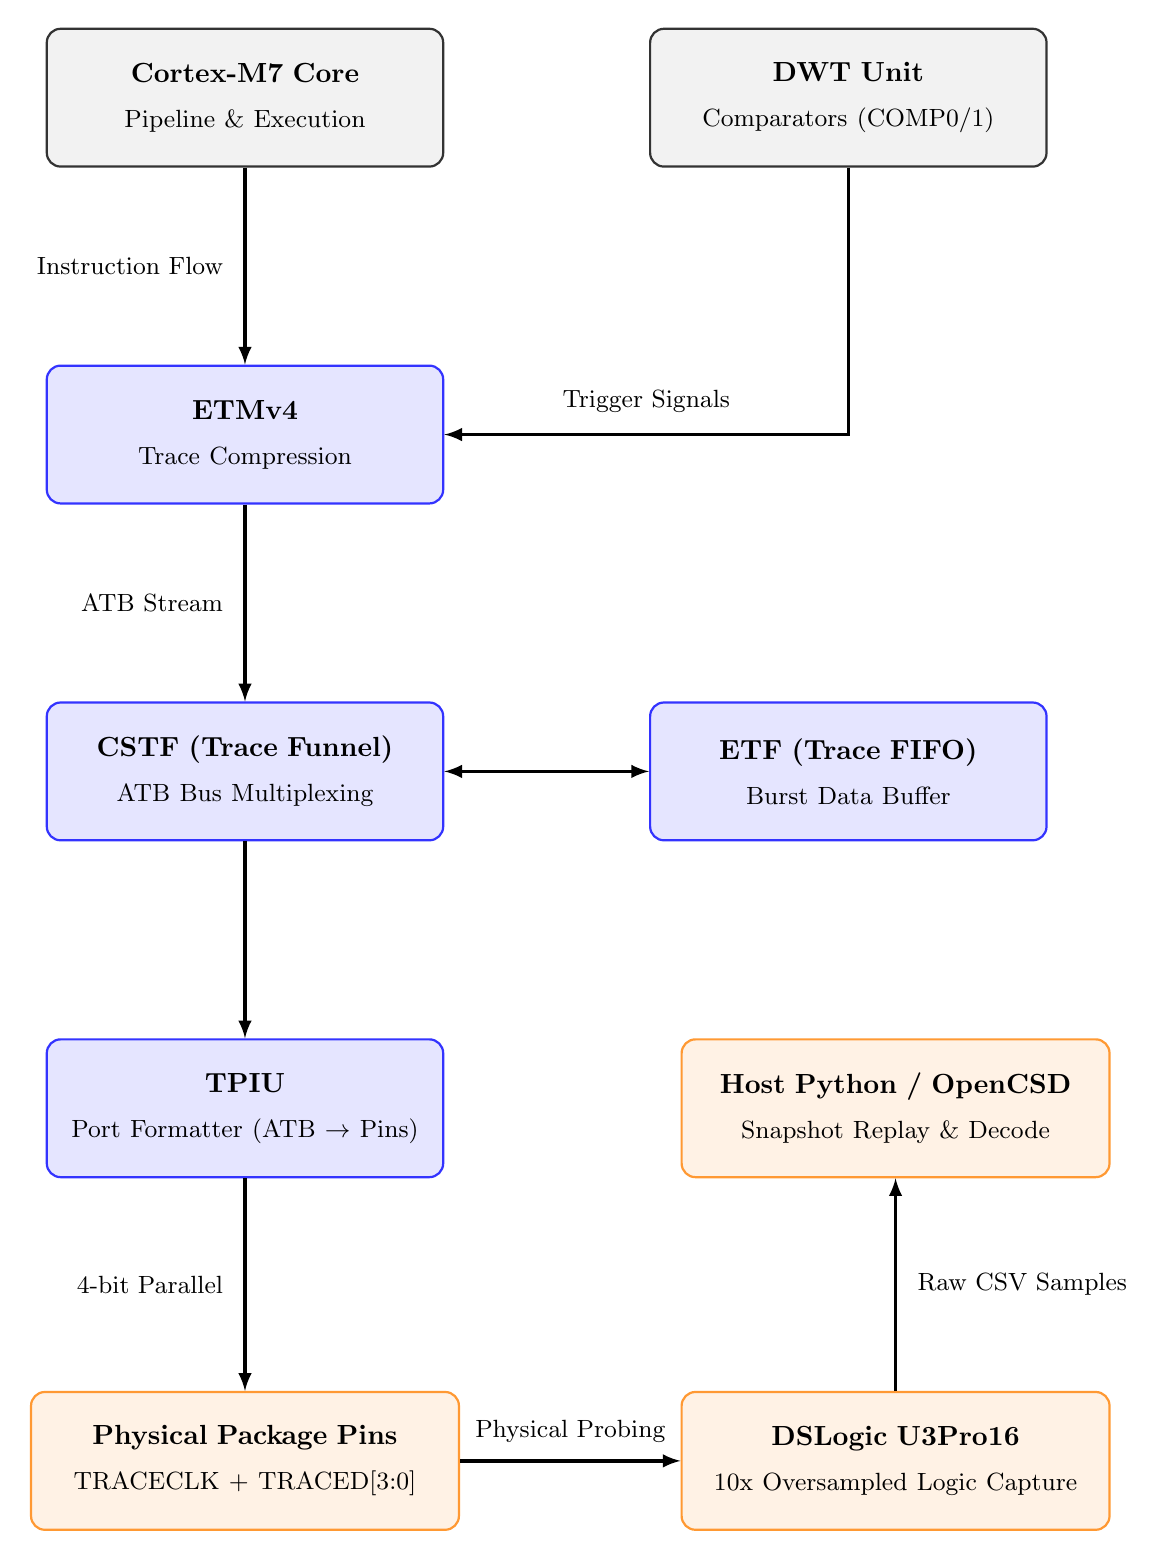
\begin{tikzpicture}[
    every node/.append style={font=\latinfont},
    node distance=2.5cm and 2.6cm,
    hw/.style={rectangle, draw=black!80, fill=gray!10, thick, rounded corners=5pt, text width=4.8cm, align=center, minimum height=1.75cm},
    trace/.style={rectangle, draw=blue!80, fill=blue!10, thick, rounded corners=5pt, text width=4.8cm, align=center, minimum height=1.75cm},
    ext/.style={rectangle, draw=orange!80, fill=orange!10, thick, rounded corners=5pt, text width=5.2cm, align=center, minimum height=1.75cm},
    arrow/.style={-latex, very thick}
]
    % On-chip Core & Trigger
    \node [hw] (core) {\textbf{Cortex-M7 Core}\\[0.15cm]\small Pipeline \& Execution};
    \node [hw, right=2.6cm of core] (dwt) {\textbf{DWT Unit}\\[0.15cm]\small Comparators (COMP0/1)};
    
    % Trace Generation
    \node [trace, below=2.5cm of core] (etm) {\textbf{ETMv4}\\[0.15cm]\small Trace Compression};
    
    % Transport
    \node [trace, below=2.5cm of etm] (cstf) {\textbf{CSTF (Trace Funnel)}\\[0.15cm]\small ATB Bus Multiplexing};
    \node [trace, right=2.6cm of cstf] (etf) {\textbf{ETF (Trace FIFO)}\\[0.15cm]\small Burst Data Buffer};
    \node [trace, below=2.5cm of cstf] (tpiu) {\textbf{TPIU}\\[0.15cm]\small Port Formatter (ATB \ensuremath{\to} Pins)};
    
    % Off-chip Pins & Analyzer
    \node [ext, below=2.7cm of tpiu] (pins) {\textbf{Physical Package Pins}\\[0.15cm]\small TRACECLK + TRACED[3:0]};
    \node [ext, right=2.8cm of pins] (dslogic) {\textbf{DSLogic U3Pro16}\\[0.15cm]\small \mbox{10x Oversampled} Logic Capture};
    \node [ext, above=2.7cm of dslogic] (host) {\textbf{Host Python / OpenCSD}\\[0.15cm]\small Snapshot Replay \& Decode};

    % Connections
    \draw [arrow] (core) -- node[left=4pt, font=\small] {Instruction Flow} (etm);
    \draw [arrow] (dwt.south) |- node[near end, above=4pt, font=\small] {Trigger Signals} (etm.east);
    \draw [arrow] (etm) -- node[left=4pt, font=\small] {ATB Stream} (cstf);
    \draw [arrow, latex-latex] (cstf) -- (etf);
    \draw [arrow] (cstf) -- (tpiu);
    \draw [arrow] (tpiu) -- node[left=4pt, font=\small] {4-bit Parallel} (pins);
    \draw [arrow] (pins) -- node[midway, above=4pt, font=\small, fill=white, inner sep=2pt] {Physical Probing} (dslogic);
    \draw [arrow] (dslogic) -- node[right=4pt, font=\small] {Raw CSV Samples} (host);
\end{tikzpicture}
\end{latin}
\caption{زنجیره کامل جریان سیگنال‌ها در معماری \lr{ARM CoreSight} از هسته پردازنده تا ابزار تحلیل}
\label{fig:coresight_pipeline}
\end{figure}

\subsection{اجزای زیرسیستم \lr{CoreSight} در \lr{STM32H750}}
\begin{enumerate}
    \item \textbf{واحد پورت دسترسی به عیب‌یابی (\lr{DAP - Debug Access Port}):} درگاه اصلی اتصال ابزارهای دیباگ خارجی از طریق رابط‌های دو سیمه \lr{SWD} یا چندسیمه \lr{JTAG} جهت دسترسی به ثبّات‌های کنترلی و فضای آدرس حافظه بدون مداخله هسته.
    \item \textbf{گذرگاه پیشرفته ردگیری (\lr{ATB - Advanced Trace Bus}):} پروتکل گذرگاه داده همگام و پرسرعت درون‌تراشه‌ای که بسته‌های ردگیری تولیدشده توسط ماژول‌های پایش را میان اجزای گوناگون منتقل می‌سازد.
    \item \textbf{واحد نگهبان داده و ردگیری (\lr{DWT - Data Watchpoint and Trace}):} ماژولی حیاتی که وظایف متعددی نظیر شمارش چرخه‌های زمانی (\lr{CYCCNT}) و مقایسه آدرس‌های حافظه را انجام می‌دهد. ثبّات‌های مقایسه‌گر \lr{DWT\_COMP0} و \lr{DWT\_COMP1} نقشی محوری در تعریف محدوده پنجره‌های پایش دارند؛ به طوری که با رسیدن آدرس اشاره‌گر دستورات به یک برچسب خاص، سیگنال شروع یا پایان ردگیری به \lr{ETM} صادر می‌گردد.
    \item \textbf{قیف ادغام ردگیری (\lr{CSTF - CoreSight Trace Funnel}):} ماژولی چندورودی-تک‌خروجی که وظیفه تلفیق جریان داده‌های ردگیری از منابع مختلف درون‌تراشه‌ای (نظیر هسته‌های چندگانه، \lr{ETM} و \lr{ITM}) به یک گذرگاه واحد \lr{ATB} را با شناسه مبدأ (\lr{Trace Source ID}) مشخص عهده‌دار است.
    \item \textbf{بافر میانی جریان داده (\lr{ETF - Embedded Trace FIFO}):} یک حافظه \lr{SRAM} حلقوی درون‌تراشه‌ای جهت جذب انفجارهای ناگهانی داده‌های \lr{Trace} (\lr{Data Bursts})؛ در زمان‌هایی که انشعاب‌های شرطی مکرر موجب افزایش نرخ تولید بسته شده و پهنای باند پورت خروجی پاسخگو نیست.
    \item \textbf{واحد واسط پورت ردیابی (\lr{TPIU - Trace Port Interface Unit}):} آخرین حلقه زنجیره درون‌تراشه‌ای که فریم‌های پروتکل \lr{ATB} را دریافت کرده، آن‌ها را با الگوهای همگام‌سازی فریم (بایت \texttt{0x7F}) بسته‌بندی نموده و به صورت جفت‌نیبل‌های موازی روی کلاک خروجی و پایه‌های خارجی تراشه منتشر می‌سازد.
\end{enumerate}

\section{پیشینه پژوهش و مقایسه تطبیقی رویکردها}
رویکردهای پایش، استخراج مسیر و ارزیابی زمان در سامانه‌های نهفته در جدول \ref{tab:trace_comparison} مورد مقایسه قرار گرفته‌اند.

\begin{table}[ht]
\centering
\small
\setlength{\tabcolsep}{3.5pt}
\renewcommand{\arraystretch}{1.45}
\caption{مقایسه تطبیقی پلتفرم‌های آزمون و ردگیری اجرای برنامه در سیستم‌های نهفته}
\label{tab:trace_comparison}
\begin{tabularx}{\textwidth}{|>{\hsize=1.3\hsize\raggedleft\arraybackslash}X|*{4}{>{\hsize=0.925\hsize\centering\arraybackslash}X|}}
\hline
\textbf{معیار مقایسه} & \textbf{ابزاردقیق نرم‌افزاری} & \textbf{شبیه‌ساز نرم‌افزاری} & \textbf{پلتفرم تجاری (\lr{Rapita/Speedgoat})} & \textbf{پلتفرم این رساله} \\
\hline
سربار زمانی \lr{(Probe Effect)} & بالا ($>15\%$) & صفر & صفر (غیرتهاجمی) & \textbf{صفر (غیرتهاجمی)} \\
\hline
تغییر کد منبع \lr{(Source Intrusion)} & نیاز دارد & بی‌نیاز & بی‌نیاز & \textbf{کاملاً بی‌نیاز} \\
\hline
دقت زمانی و رفتار چرخه‌ای & مخدوش و دارای جیتر & تقریبی & چرخه دقیق & \textbf{چرخه دقیق (جیتر صفر)} \\
\hline
هزینه لایسنس و سامانه آزمون & ناچیز & ناچیز & بسیار بالا ($>\$10,000$) & \textbf{حداقل هزینه (اقتصادی)} \\
\hline
وابستگی به برنامه کامپایل‌شده & بالا & کامل & فقط فایل باینری & \textbf{فقط باینری (\lr{.elf})} \\
\hline
پشتیبانی از پایش وقفه‌ها & نامطمئن & وابسته به مدل & کامل & \textbf{کامل و تفکیک‌شده} \\
\hline
\end{tabularx}
\end{table}

همان‌گونه که از جدول \ref{tab:trace_comparison} برمی‌آید، در صنایع هوافضا، خودروسازی و اتوماسیون پیشرفته، پلتفرم‌های تجاری آزمون خودکار محصول و تحلیل زمان‌بندی (نظیر محصولات \lr{Rapita Systems} و بسترهای \lr{Speedgoat}) استاندارد طلایی به شمار می‌روند؛ اما استقرار این پلتفرم‌ها نیازمند هزینه‌های بسیار سنگین (ده‌ها هزار دلار) و تجهیزات انحصاری است. یکی از مهم‌ترین اهداف و دستاوردهای محصول مشترک این پژوهش و پروژه همگام (سامانه آزمون خودکار)، تحقق یک پلتفرم آزمون محصول کارا و ارزان‌قیمت است که توانسته فرآیند آزمون نرم‌افزار، ماک‌سازی پریفرال‌ها و استخراج مسیر اجرا را با حداقل هزینه محقق سازد.

همچنین در سطح سخت‌افزار دریافت سیگنال، اگرچه پروب‌های سخت‌افزاری تجاری نظیر \lr{SEGGER J-Trace} به ثبت مستقیم در فرکانس‌های بالا می‌پردازند، اما درون آن‌ها از تراشه‌های اختصاصی \lr{FPGA} و حافظه‌های سریع \lr{DRAM} استفاده شده است. آزمون‌های تجربی این پروژه نشان داد که لاجیک‌آنالایزرهای عمومی اقتصادی نهایتاً برای فرکانس‌های بسیار بالا ایده‌آل نبوده و بهترین انتخاب سخت‌افزاری، یک برد سفارشی مبتنی بر \lr{FPGA} است؛ هرچند هزینه پیاده‌سازی اختصاصی آن با هزینه خرید پروب‌های تجاری تقریباً برابری خواهد کرد. با این حال، ارزش افزوده اصلی این رساله، توسعه کل چرخه نرم‌افزاری استخراج و دیکودینگ داده‌ها با هزینه بسیار پایین است.

\section{جمع‌بندی فصل}
در این فصل پایه‌های تئوریک محاسبه \lr{WCET} و ساختار لایه‌ای معماری \lr{ARM CoreSight} تشریح گردید. همچنین ضرورت اجتناب از ابزاردقیق نرم‌افزاری و مزایای اقتصادی و فنی پلتفرم توسعه‌داده‌شده نسبت به راهکارهای تجاری گران‌قیمت بازار مورد ارزیابی قرار گرفت. با استناد به این مبانی، در فصل سوم به طراحی معماری کلان سامانه و پیاده‌سازی گام‌به‌گام خط لوله تأمین داده پرداخته خواهد شد.


% فصل سوم: معماری کلان سامانه
% ==============================================================================
% فصل سوم: معماری کلان سامانه
% ==============================================================================

\chapter{معماری کلان سامانه}
\label{ch:architecture}

\section{مقدمه}
طراحی و پیاده‌سازی یک خط‌لوله داده جهت استنتاج بدترین حالت زمان اجرا (\lr{WCET}) در سامانه‌های نهفته بی‌درنگ، نیازمند اتخاذ تصمیمات بنیادین معماری، تفکیک دقیق وظایف میان زیرسیستم‌های سخت‌افزاری و نرم‌افزاری، و ایجاد یک بستر عملیاتی بدون سربار است. در این فصل، ابتدا مسیر تکامل پژوهش و دلایل فنی گذار از بردهای مبتنی بر \lr{RP2350} به میکروکنترلر صنعتی \lr{STM32H750} تبیین می‌گردد. سپس نیازمندی‌های کارکردی و کیفی سامانه استخراج شده و معماری کلان سامانه به همراه نحوه تعامل و تبادل داده با سامانه آزمون خودکار (پروژه مکمل) با جزئیات فنی تشریح می‌شود.

\section{مسیر تکامل سخت‌افزار: از \lr{RP2350 (Pico 2)} تا \lr{STM32H750}}
\label{sec:arch_evolution}
در فاز مطالعاتی اولیه این پژوهش، تمرکز بر بهره‌گیری از میکروکنترلر نوین \lr{Raspberry Pi Pico 2} (مبتنی بر تراشه \lr{RP2350}) قرار داشت. تراشه \lr{RP2350} با ساختار دوهسته‌ای ترکیبی (\lr{ARM Cortex-M33} و \lr{Hazard3 RISC-V}) گزینه‌ای جذاب و اقتصادی به نظر می‌رسید. هدف اولیه، راه‌اندازی واحد \lr{ETM} موجود در هسته \lr{Cortex-M33} و خواندن داده‌های ردگیری از طریق یک لایه میان‌افزار (\lr{Middleware}) یا اسکریپت‌های کامپایلر بود؛ به نحوی که کد اصلی کاربر به زبان \lr{C} کاملاً دست‌نخورده باقی بماند.

با این حال، در جریان پیشبرد عملیاتی این راهکار، موانع فنی بازدارنده‌ای شناسایی گردید:
\begin{enumerate}
    \item \textbf{نقص مستندات و ناپختگی تراشه \lr{RP2350}:} با توجه به عرضه بسیار جدید تراشه \lr{RP2350}، مستندات رسمی مربوط به ثبّات‌های نگاشت‌شده درگاه‌های عیب‌یابی \lr{CoreSight}، ماتریس اتصال سوییچ‌های \lr{ATB}، و ساختار داخلی \lr{ETM} در زمان اجرای پروژه بسیار محدود، ناقص و همراه با اراتا‌های سخت‌افزاری متعدد بود.
    \item \textbf{عدم دسترسی به پایه‌های فیزیکی \lr{Trace} در بردهای تجاری:} بزرگ‌ترین چالش فیزیکی، عدم هدایت پایه‌های موازی \lr{TPIU} به پین‌هدرهای خروجی برد تجاری \lr{Pico 2} بود. بردهای توسعه تجاری تنها پایه‌های دو سیمه \lr{SWD} و پورت سریال \lr{UART} را به بیرون هدایت کرده بودند؛ در حالی که پورت ردیابی پیوسته نیازمند دسترسی بدون واسطه به حداقل ۵ پایه سخت‌افزاری \lr{Trace} (یک کلاک و ۴ خط داده) بود. دسترسی به این پایه‌ها نیازمند لحیم‌کاری‌های میکرومتری روی پکیج \lr{QFN} بود که ریسک نویز، عدم تطبیق امپدانس و ناپایداری سیگنال را به شدت افزایش می‌داد.
    \item \textbf{محدودیت شدید پهنای باند و بافر ذخیره‌سازی در \lr{RP2350}:} در تراشه رزبری پای، پهنای باند و حافظه بافر اختصاصی سخت‌افزاری برای ذخیره‌سازی و خروجی دادن داده‌های \lr{Trace} بسیار محدود است. این گلوگاه موجب می‌شد که استخراج داده‌های ردیابی مستلزم مداخله نرم‌افزاری در روند اجرای برنامه و درگیر کردن یکی از هسته‌های پردازنده به عنوان واسط ذخیره‌سازی یا ارسال داده باشد. این درگیرسازی نرم‌افزاری و اشغال هسته، شرط بنیادین عدم مداخله و اصل غیرتهاجمی بودن (\lr{Non-intrusive}) را کاملاً نقض می‌کرد و رفتار زمانی سیستم را به شکل نامطلوبی تغییر می‌داد.
    \item \textbf{جامعیت و بلوغ صنعتی خانواده \lr{STM32}:} در سوی مقابل، شرکت \lr{STMicroelectronics} در خانواده میکروکنترلرهای مبتنی بر \lr{ARM Cortex-M7} (به‌ویژه سری \lr{STM32H750}) ساختار استاندارد، بالغ و کاملاً مستندشده \lr{CoreSight ETMv4} را ارائه می‌دهد. در این پردازنده‌ها، پایه‌های پورت موازی \lr{TPIU} به عنوان توابع جانبی جایگزین (\lr{Alternate Function 0}) بر روی پورت \lr{E} (پایه‌های \lr{\texttt{PE2}} الی \lr{\texttt{PE6}}) تعبیه شده‌اند و دسترسی سخت‌افزاری کاملاً پایدار را ممکن می‌سازند.
\end{enumerate}

بنابراین، تصمیم راهبردی معماری بر گذار کامل به میکروکنترلر \lr{STM32H750VBT6} اتخاذ گردید تا تمرکز پژوهش بر هسته علمی استنتاج غیرتهاجمی و پردازش سیگنال‌های \lr{Trace} متمرکز بماند.

\section{تحلیل جامع نیازمندی‌های سامانه}
برای تضمین صحت عملکرد در محیط‌های بی‌درنگ سخت، نیازمندی‌های سامانه در دو دسته کارکردی و کیفی تدوین گردید:

\subsection{نیازمندی‌های کارکردی (\lr{Functional Requirements})}
\begin{enumerate}
    \item \textbf{پیکربندی غیرتهاجمی زیرسیستم \lr{CoreSight}:} فعال‌سازی، تنظیم ثبّات‌های کنترلی، باز کردن قفل دسترسی (\lr{LAR}) و تعیین فیلترهای رویداد بدون تزریق حتی یک خط کد اضافه به باینری نرم‌افزار هدف.
    \item \textbf{پیکربندی جامع و مناسب تمامی بلوک‌های زنجیره \lr{Trace}:} مقداردهی هماهنگ و سازگار کلیه واحدهای سخت‌افزاری فعال در خط‌لوله شامل \lr{DBGMCU}، \lr{TPIU}، قیف ادغام داده‌ها (\lr{CSTF}) و هسته \lr{ETMv4} بدون ایجاد تناقض یا بن‌بست در جریان داده‌ها.
    \item \textbf{قابلیت تنظیم محل و طول پنجره ردیابی توسط کاربر:} فراهم ساختن امکان تعیین دقیق نقاط شروع و پایان فرآیند ردگیری (تعیین پنجره زمانی یا بازه آدرس‌های اجرایی هدف) توسط کاربر، جهت متمرکز شدن بر بخش‌های بحرانی کد و بهینه‌سازی حجم داده‌های ثبتی.
    \item \textbf{هدایت موازی جریان \lr{Trace} از پورت فیزیکی \lr{TPIU}:} ارسال بایت‌های فشرده‌شده داده از طریق رابط ۵ سیمه سنکرون (\lr{TRACECLK} و \lr{TRACED[0:3]}).
    \item \textbf{بازسازی دقیق جریان بیت‌ها به بایت‌های پروتکل:} نمونه‌برداری با فرکانس متناسب، آشکارسازی لبه‌ها و بازیابی جفت‌نیبل‌های فریم‌بندی‌شده.
    \item \textbf{همگام‌سازی اجباری در پنجره‌های کوتاه آزمون:} حل چالش عدم همگام‌سازی (\lr{A-Sync}) در روتین‌های وقفه و توابع میکروثانیه‌ای.
    \item \textbf{بازسازی جریان کامل دستورات با موتور استاندارد:} ادغام با کتابخانه صنعتی \lr{OpenCSD}، نگاشت نمادهای فایل باینری (\lr{ELF})، و استخراج گام‌به‌گام دستورات اسمبلی.
    \item \textbf{شمارش دقیق چرخه‌های پردازنده (\lr{Cycle-Accurate Timing}):} انتساب برچسب زمانی و چرخه‌های کلاک سپری‌شده به هر بلوک محاسباتی و روتین‌های وقفه.
\end{enumerate}

\subsection{نیازمندی‌های کیفی و غیرکارکردی (\lr{Non-Functional Requirements})}
\begin{itemize}
    \item \textbf{عدم قطعیت و جیتر صفر (\lr{Zero Jitter}):} سیستم مانیتورینگ نباید رفتار زمانی پردازنده را متغیر سازد؛ زمان‌های اندازه‌گیری‌شده در شرایط ورودی یکسان باید در سطح چرخه ماشین (\lr{Cycle-deterministic}) کاملاً تکرارپذیر باشند.
    \item \textbf{نرخ خطای صفر در بازسازی (\lr{Zero Decode Error}):} از دست رفتن حتی یک بایت یا خطا در تصمیم یک انشعاب شرطی، کل مسیر اجرای پس از آن را نامعتبر می‌سازد؛ از این رو نرخ خطای رمزگشایی در سناریوهای طولانی باید اکیداً صفر باشد.
    \item \textbf{قابلیت اتکا و کاهش هزینه سخت‌افزاری:} پرهیز از پروب‌های صنعتی انحصاری با قیمت چندهزار دلاری و جایگزینی آن با سخت‌افزارهای اقتصادی در دسترس.
\end{itemize}

\clearpage
\section{معماری کلان و لایه‌های شش‌گانه سامانه}
\label{sec:six_layers_arch}
سامانه تأمین داده‌های ردیابی در قالب یک معماری شش‌لایه‌ای سلسله‌مراتبی مهندسی شده است. شکل \ref{fig:detailed_arch_flow} جریان تبدیل داده را از نانوثانیه‌های پالس‌های فیزیکی سیلیکون تا ماتریس‌های ساخت‌یافته تحلیل \lr{WCET} به تصویر می‌کشد.

\begin{figure}[H]
\centering
\begin{latin}
\centering
\begin{tikzpicture}[
    node distance=1.1cm,
    layer/.style={rectangle, draw=blue!75!black, fill=blue!5, thick, rounded corners=4pt, text width=13.8cm, align=center, inner sep=3.5pt},
    arrow/.style={-latex, very thick, draw=black!70}
]
    \node [layer] (L1) {
        \rl{\textbf{لایه ۱: هسته محاسباتی و فشرده‌سازی درون‌تراشه}} \\
        \lr{\textbf{(Layer 1: On-Chip Core \& ETMv4)}} \\[0.05cm]
        \small \rl{اجرای برنامه‌های آزمون، پایش انشعاب‌ها توسط \lr{ETMv4}، تولید بسته‌های اتم، درج شمارنده‌های چرخه}
    };
    
    \node [layer, below=0.35cm of L1] (L2) {
        \rl{\textbf{لایه ۲: تعیین گذرگاه و فرمت‌بندی پورت}} \\
        \lr{\textbf{(Layer 2: ATB / CSTF / TPIU)}} \\[0.05cm]
        \small \rl{تعیین داده‌ها از طریق \lr{CSTF}، مدیریت بافر \lr{ETF}، تبدیل جریان به جفت‌نیبل و درج بایت همگام‌سازی \lr{\texttt{0x7F}}}
    };
    
    \node [layer, below=0.35cm of L2] (L3) {
        \rl{\textbf{لایه ۳: بستر فیزیکی و سیگنال‌های پین‌ها}} \\
        \lr{\textbf{(Layer 3: Physical Trace Interface)}} \\[0.05cm]
        \small \rl{پایه‌های پورت \lr{\texttt{PE2..PE6}}، انطباق امپدانس، کنترل نرخ صعود، و اتصال به پین‌های خروجی و سیم‌کشی \lr{Trace}}
    };
    
    \node [layer, below=0.35cm of L3] (L4) {
        \rl{\textbf{لایه ۴: دریافت و نمونه‌برداری لاجیک‌آنالایزر}} \\
        \lr{\textbf{(Layer 4: 10x Oversampled Logic Capture)}} \\[0.05cm]
        \small \rl{دستگاه \lr{DSLogic U3Pro16}، نمونه‌برداری ۱۰ برابری نسبت به کلاک \lr{Trace}، حذف نویز و استخراج فایل نمونه‌های \lr{CSV}}
    };
    
    \node [layer, below=0.35cm of L4] (L5) {
        \rl{\textbf{لایه ۵: ماژول پردازش جریان \lr{Trace}}} \\
        \lr{\textbf{(Layer 5: TraceStreamProcessor.py)}} \\[0.05cm]
        \small \rl{آشکارسازی لبه‌های کلاک، تجمیع نیبل‌ها به بایت، اعتبارسنجی فریم‌های \lr{TPIU}، و ساختارمند کردن پوشه اسنپ‌شات \lr{OpenCSD}}
    };
    
    \node [layer, below=0.35cm of L5] (L6) {
        \rl{\textbf{لایه ۶: موتور رمزگشای مرجع و نگاشت کد}} \\
        \lr{\textbf{(Layer 6: OpenCSD Engine \& Disassembly Matching)}} \\[0.05cm]
        \small \rl{دیکود عمیق بسته‌ها، تطبیق با باینری \lr{ELF}، بازسازی مسیر اجرای دستورات و تحویل ماتریس به سامانه تحلیل \lr{WCET}}
    };

    \draw [arrow] (L1) -- (L2);
    \draw [arrow] (L2) -- (L3);
    \draw [arrow] (L3) -- (L4);
    \draw [arrow] (L4) -- (L5);
    \draw [arrow] (L5) -- (L6);
\end{tikzpicture}
\end{latin}
\caption{معماری شش‌لایه‌ای سامانه تأمین داده از هسته سخت‌افزار تا موتور رمزگشایی}
\label{fig:detailed_arch_flow}
\end{figure}
\clearpage

\section{مرزبندی معماری و تعامل با سامانه آزمون خودکار (پروژه مکمل)}
\label{sec:dual_arch_interaction}
پروژه حاضر (سامانه تأمین داده‌های ردیابی) و پروژه مکمل (سامانه آزمون خودکار) به گونه‌ای طراحی شده‌اند که دو سامانه کاملاً ماژولار، تفکیک‌شده و با مرزبندی صریح معماری (\lr{Separation of Concerns}) باشند.

\subsection{حفظ اصالت کدهای کاربر و بازنگاشت در لایه میانی}
یکی از شروط بنیادین در ارزیابی رفتارهای زمانی سیستم‌های نهفته، اجتناب از دستکاری کد اصلی برنامه کاربر است. در پروژه مکمل، شبیه‌سازی و تحریک مقادیر پریفرال‌های خارجی بدون تغییر در کدهای اصلی کاربر و صرفاً از طریق بازتعریف توابع لایه میانی \lr{HAL} صورت گرفته است؛ به نحوی که ثبّات‌های پریفرال به بخش دیگری از حافظه بازنگاشت (\lr{Remap}) شده و داده‌های آزمون بدون نیاز به تغییر منطق سورس‌کد به برنامه خورانده می‌شوند.

\subsection{استقلال عملیاتی و پروتکل تبادل داده}
معماری و پارتیشن‌بندی میان این دو پروژه به گونه‌ای پیاده‌سازی شده است که کارکرد هر دو سامانه به طور کامل از یکدیگر مستقل باشد و ارتباط آن‌ها صرفاً به تبادل استاندارد داده محدود گردد. سامانه تأمین داده به عنوان یک ناظر سخت‌افزاری کاملاً مستقل عمل می‌کند که هیچ وابستگی به منطق آزمون ندارد؛ وظیفه این سامانه منحصراً ثبت سیگنال‌های فیزیکی، بازسازی جریان دستورات و تحویل ماتریس ساخت‌یافته ردگیری اجرای برنامه (\lr{Execution Trace Matrix}) است:
\begin{equation}
\label{eq:trace_matrix}
\mathcal{M}_{\mathrm{trace}} = \left\{ \left( \mathrm{PC}_k, \; \Delta t_k, \; \mathrm{BranchTaken}_k, \; \mathrm{Context}_k \right) \right\}_{k=1}^{M}
\end{equation}
در این رابطه، $\mathrm{PC}_k$ آدرس ۳۲ بیتی شمارنده برنامه، $\Delta t_k$ تعداد چرخه‌های کلاک سپری‌شده بین رخدادها، $\mathrm{BranchTaken}_k$ وضعیت تحقق یا عدم تحقق انشعاب شرطی، و $\mathrm{Context}_k$ شناسه زمینه اجرایی پردازنده است. این ماتریس به عنوان خروجی رسمی سامانه تأمین داده در اختیار سامانه مکمل قرار می‌گیرد تا برای هدایت آزمون‌های بعدی و استنتاج بدترین حالت زمان اجرا (\lr{WCET}) به کار گرفته شود. مدل مفهومی مرزبندی معماری و نحوه تعامل بدون مداخله میان این دو سامانه در شکل \ref{fig:closed_loop_interaction} به تصویر کشیده شده است.

\begin{figure}[H]
\centering
\begin{latin}
\centering
\begin{tikzpicture}[
    box/.style={rectangle, draw=blue!80!black, fill=blue!5, thick, rounded corners=5pt, text width=5.6cm, align=center, minimum height=1.9cm, inner sep=4pt},
    auxbox/.style={rectangle, draw=orange!80!black, fill=orange!5, thick, rounded corners=5pt, text width=5.6cm, align=center, minimum height=1.9cm, inner sep=4pt},
    hwbox/.style={rectangle, draw=green!60!black, fill=green!5, thick, rounded corners=5pt, text width=14.2cm, align=center, minimum height=1.6cm, inner sep=4pt},
    line/.style={draw=black!75, -latex, thick}
]
    \node [box] (provider) at (-4.3, 4.8) {
        \rl{\textbf{سامانه تأمین داده‌های ردیابی}}\\[0.08cm]
        \small \rl{ثبت سخت‌افزاری پایه‌های \lr{ETMv4}}\\[0.04cm]
        \small \rl{پردازش با \lr{TraceStreamProcessor}}\\[0.04cm]
        \small \rl{بازسازی جریان دستورات با \lr{OpenCSD}}
    };
    
    \node [auxbox] (tester) at (4.3, 4.8) {
        \rl{\textbf{سامانه آزمون خودکار (پروژه مکمل)}}\\[0.08cm]
        \small \rl{تولید هدایت‌شده بردارهای ورودی}\\[0.04cm]
        \small \rl{بازنگاشت ثبّات‌ها در لایه میانی \lr{HAL}}\\[0.04cm]
        \small \rl{محاسبه و استنتاج \lr{WCET}}
    };

    \node [hwbox] (target) at (0, 0) {
        \rl{\textbf{میکروکنترلر هدف صنعتی}}\\[0.06cm]
        \lr{\textbf{STM32H750VBT6 (ARM Cortex-M7)}}\\[0.06cm]
        \small \rl{اجرای کد دست‌نخورده کاربر و انتشار برخط پالس‌های \lr{Trace} از پایه‌های} \lr{\texttt{PE2..PE6}}
    };

    % Paths
    \draw [line] (tester.south) -- node [left=0.15cm, midway, align=right, font=\scriptsize] {\rl{تزریق ورودی‌ها}\\\rl{به لایه میانی}} (tester.south |- target.north);
    \draw [line] (provider.south |- target.north) -- node [right=0.15cm, midway, align=left, font=\scriptsize] {\rl{ردیابی سخت‌افزاری}\\\lr{TRACECLK + TRACED[0:3]}} (provider.south);
    \draw [line, dashed] (provider.east) -- node [above=0.08cm, midway, align=center, font=\scriptsize] {\rl{ماتریس خروجی ردگیری}} node [below=0.08cm, midway, align=center, font=\scriptsize] {$\mathcal{M}_{\mathrm{trace}} \to \text{\rl{استنتاج}}\;\mathrm{WCET}$} (tester.west);
\end{tikzpicture}
\end{latin}
\caption{مدل مرزبندی معماری و تبادل داده میان سامانه تأمین داده و سامانه آزمون مکمل}
\label{fig:closed_loop_interaction}
\end{figure}

\section{معماری نهایی سامانه}
\label{sec:final_system_architecture}
پیرو تحلیل نیازمندی‌ها، تفکیک لایه‌های شش‌گانه پردازش داده و تبیین مدل مرزبندی با سامانه آزمون مکمل، پیکربندی عملیاتی کل سیستم نیازمند یک بلوک‌دیاگرام جامع معماری است که مرزهای فیزیکی، جایگاه دقیق دستگاه‌های ابزاردقیق و اندازه‌گیری، و خط‌لوله پردازش نرم‌افزاری میزبان را به وضوح نشان دهد. ساختار عملیاتی سامانه در سه بخش بنیادین (سخت‌افزار هدف، لایه اندازه‌گیری و ابزاردقیق، و سامانه نرم‌افزاری میزبان) سازمان‌دهی شده است:

\begin{enumerate}
    \item \textbf{بخش اول: سخت‌افزار هدف تحت آزمون (\lr{Target Hardware / DUT}):}
    میکروکنترلر صنعتی \lr{STM32H750VBT6} که مجهز به هسته محاسباتی پیشرفته \lr{ARM Cortex-M7} است. کدهای کاربر بدون نیاز به هیچ‌گونه ابزاردقیق نرم‌افزاری یا تزریق پروب‌های آلوده‌کننده زمان، با رفتار اصیل خود اجرا می‌شوند. ماژول آن‌چیپ \lr{ETMv4} با پایش بی‌درنگ خط‌لوله دستورات، اطلاعات شاخه‌ها (\lr{Atom Packets})، شمارنده چرخه‌ها (\lr{CCI}) و برچسب‌های زمانی سراسری (\lr{TS}) را تولید کرده و از طریق گذرگاه ۳۲ بیتی \lr{ATB} به سمت قيف ادغام داده‌ها (\lr{CSTF}) و بافر حلقوی \lr{ETF} گسیل می‌دارد. در نهایت، واحد واسط پورت ردیابی (\lr{TPIU}) این بسته‌ها را در فریم‌های ۱۶ بایتی استاندارد سازمان‌دهی نموده و به صورت یک گذرگاه موازی ۴ بیتی سنکرون (شامل پایه \lr{PE2} به عنوان کلاک خروجی \lr{TRACECLK} و پایه‌های \lr{PE3..PE6} به عنوان خطوط موازی داده \lr{TRACED[0:3]}) بدون تحمیل کوچک‌ترین سربار محاسباتی یا توقف هسته به بیرون صادر می‌کند.

    \item \textbf{بخش دوم: تجهیزات اندازه‌گیری و ثبت فیزیکی سیگنال‌ها (\lr{Measurement \& Acquisition Instrumentation}):}
    این بخش به عنوان پل واسط فیزیکی میان میکروکنترلر هدف و رایانه میزبان عمل می‌نماید و شامل مؤلفه‌های سخت‌افزاری زیر است:
    \begin{itemize}
        \item \textbf{پروب‌های پرسرعت با طول کم:} کابل‌های رابط شیلددار با طول کمتر از ۱۰ سانتی‌متر جهت جلوگیری از نوسانات پله‌ای (\lr{Ringing}) و انطباق امپدانس به پایه‌های پورت \lr{E} میکروکنترلر و پین‌های زمین مجاور متصل شده‌اند.
        \item \textbf{دستگاه لاجیک‌آنالایزر سخت‌افزاری (\lr{DSLogic U3Pro16}):} ثبت الکتریکی سیگنال‌های فرکانس‌بالا بر عهده این ابزار صنعتی ۱۶ کاناله قرار دارد. این دستگاه با بهره‌گیری از یک بافر آن‌بورد ۲ گیگابیتی \lr{DDR3 DRAM} و استراتژی نمونه‌برداری ناهمگام ۱۰ برابری ($10\times$ \lr{Asynchronous Oversampling})، پالس‌های ساعت و داده را با دقت بسیار بالا ثبت کرده و اثرات جیتر و لغزش فاز را در مبدأ خنثی می‌سازد.
        \item \textbf{درگاه پرسرعت \lr{USB 3.0}:} داده‌های نمونه‌برداری شده با پهنای باند بالای ۵ گیگابیت بر ثانیه و در مد استریم پیوسته و بدون سرریز، از لاجیک‌آنالایزر به رایانه میزبان منتقل می‌شوند.
    \end{itemize}

    \item \textbf{بخش سوم: سامانه نرم‌افزاری میزبان و رپر یکپارچه‌ساز (\lr{Host Processing System \& Studio Wrapper}):}
    در رایانه میزبان (\lr{Host PC})، افزونه اختصاصی \lr{CoreSight Trace Studio} به عنوان یک محیط یکپارچه توسعه و رپر جامع (\lr{Toolchain Wrapper}) در محیط \lr{VS Code} عمل می‌کند. این ابزار به جای قرارگیری صرف در انتهای خط‌لوله، به عنوان یک چتر نرم‌افزاری دربرگیرنده کل مؤلفه‌های پردازشی عمل نموده و خط‌لوله را مدیریت می‌نماید:
    \begin{itemize}
        \item \textbf{موتور پیش‌پردازش پایتون (\lr{\texttt{TraceStreamProcessor.py}}):} فایل نمونه‌های خام لاجیک‌آنالایزر را دریافت و پردازش نموده، لبه‌های معتبر کلاک را با فیلتر هوشمند گلیچ استخراج می‌کند، نیبل‌های ۴ بیتی را به بایت‌های پروتکل تجمیع می‌نماید، فریم‌ها را بر پایه الگوهای \lr{FSYNC/HSYNC} تراز فاز می‌کند و با تفکیک سگمنت‌های بارگذاری از باینری \lr{ELF}، بسته اسنپ‌شات استاندارد \lr{OpenCSD} را تولید می‌نماید.
        \item \textbf{موتور رمزگشای مرجع (\lr{OpenCSD Library}):} با فراخوانی مانیفست‌های اسنپ‌شات و اجرای ابزار استاندارد \lr{trc\_pkt\_lister}، جریان بسته‌های ردیابی و باینری برنامه را ادغام کرده و دنباله دقیق دستورات اسمبلی، برچسب‌های زمانی و شمارش چرخه‌ها را بازسازی می‌کند.
        \item \textbf{کنسول کنترلی و داشبورد استودیو (\lr{Trace Studio Dashboard}):} این پوسته یکپارچه، فرآیند تزریق خودکار درایورها به کد منبع، نشانه‌گذاری پنجره‌های پایش، هماهنگی اجرای خط‌لوله و مصورسازی زنده شاخص‌های کلیدی کارایی (\lr{KPI}) نظیر تعداد دستورات، مجموع چرخه‌ها، میانگین \lr{CPI} و بیشینه زمان اجرا را در قالبی تعاملی محقق می‌سازد.
    \end{itemize}
\end{enumerate}

خروجی نهایی این معماری، ماتریس جامع ردگیری اجرای برنامه ($\mathcal{M}_{\mathrm{trace}}$) است که به سامانه آزمون خودکار تحویل داده می‌شود تا به عنوان سنگ‌بنای ریاضی جهت استنتاج نهایی \lr{WCET} مورد بهره‌برداری قرار گیرد.

شکل \ref{fig:final_full_architecture} معماری نهایی و انتها-به-انتهای پلتفرم تأمین داده را با نمایش رپر یکپارچه‌ساز \lr{CoreSight Trace Studio} و تعامل لایه‌ها به تصویر می‌کشد.

\begin{figure}[H]
\centering
\begin{latin}
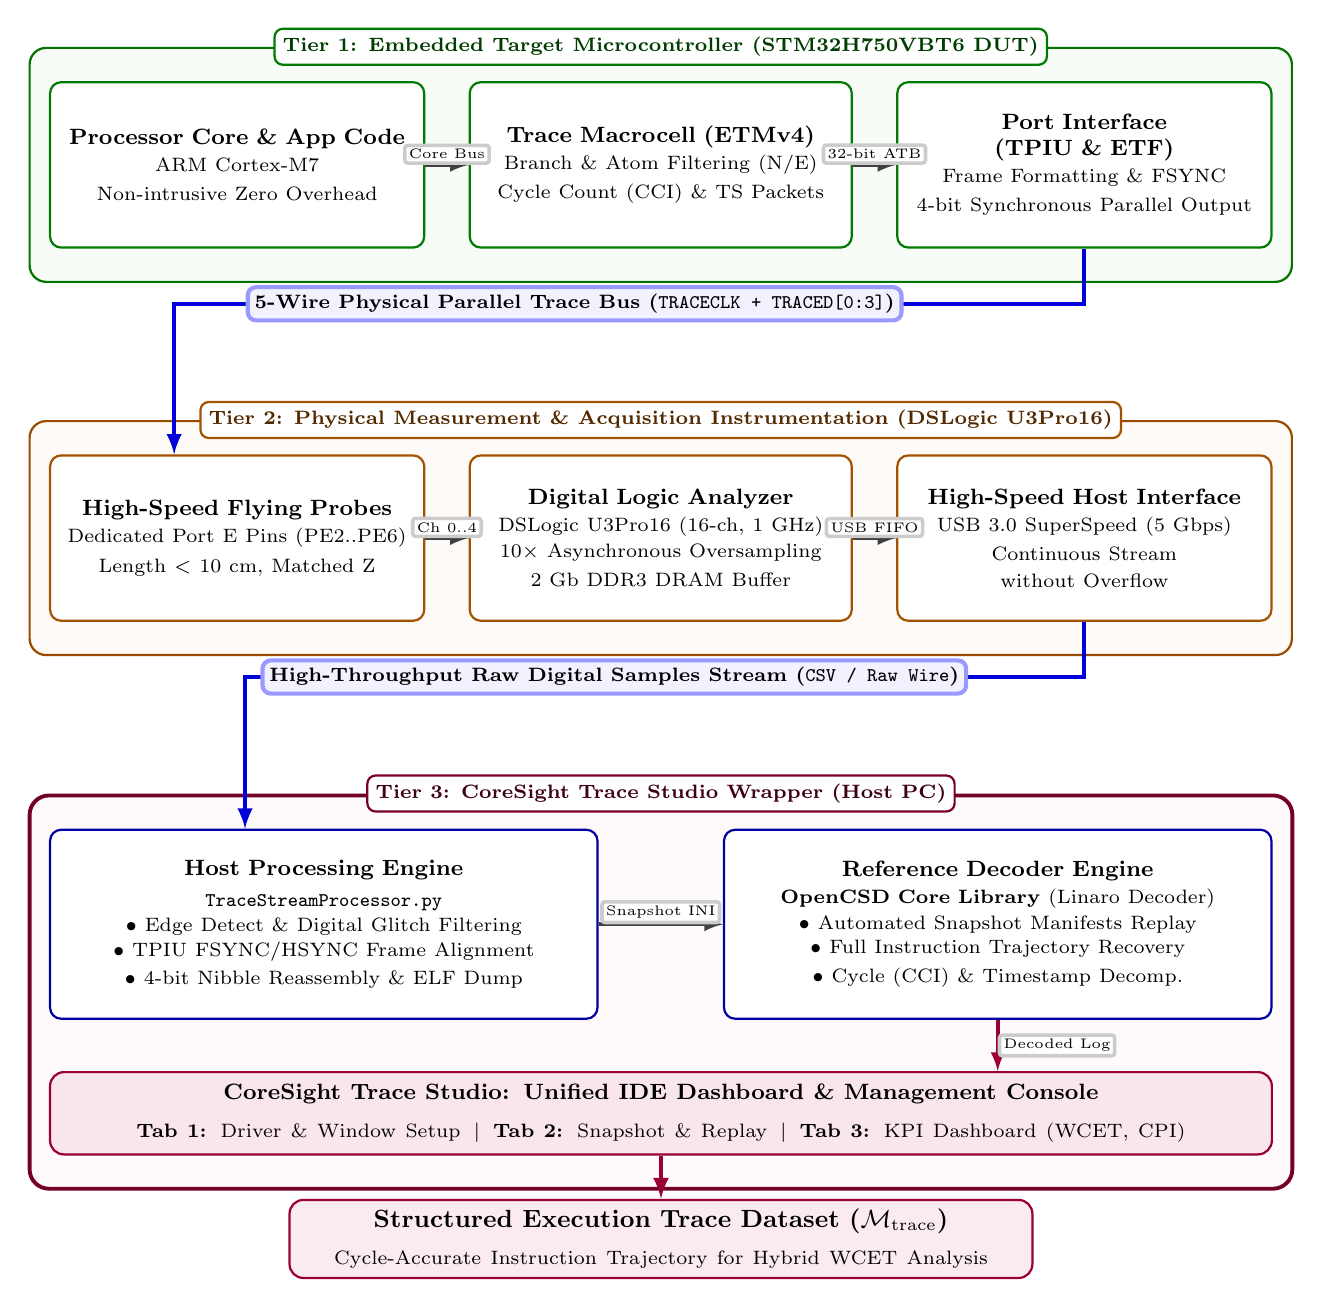
\begin{tikzpicture}[
    >=latex,
    tierbox/.style={rectangle, draw=#1!75!black, fill=#1!3, thick, rounded corners=6pt, inner ysep=12pt, inner xsep=7pt},
    tierbadge/.style={fill=white, draw=#1!80!black, thick, rounded corners=3pt, font=\bfseries\scriptsize, text=#1!40!black, inner sep=3pt},
    mod/.style={rectangle, draw=#1!80!black, fill=white, thick, rounded corners=4pt, align=center, inner sep=5pt, font=\footnotesize},
    bus/.style={draw=black!75, line width=1.3pt, ->},
    databoot/.style={draw=blue!85!black, line width=1.5pt, ->},
    buslabel/.style={font=\tiny, fill=white, inner sep=1.5pt, draw=gray!40, rounded corners=1pt},
    signallabel/.style={font=\scriptsize\bfseries, align=center, fill=blue!5, inner sep=2.5pt, draw=blue!40, rounded corners=3pt}
]

    % =========================================================================
    % TIER 1: Embedded Target Hardware (DUT)
    % =========================================================================
    \node [mod=green!60!black, text width=4.4cm, minimum height=2.1cm] (core) at (0, 0) {
        \textbf{Processor Core \& App Code} \\[0.06cm]
        \scriptsize ARM Cortex-M7\\[0.04cm]
        \scriptsize Non-intrusive Zero Overhead
    };
    \node [mod=green!60!black, text width=4.5cm, minimum height=2.1cm, right=0.55cm of core.north east, anchor=north west] (etm) {
        \textbf{Trace Macrocell (ETMv4)} \\[0.06cm]
        \scriptsize Branch \& Atom Filtering (N/E) \\[0.04cm]
        \scriptsize Cycle Count (CCI) \& TS Packets
    };
    \node [mod=green!60!black, text width=4.4cm, minimum height=2.1cm, right=0.55cm of etm.north east, anchor=north west] (tpiu) {
        \textbf{Port Interface (TPIU \& ETF)} \\[0.06cm]
        \scriptsize Frame Formatting \& FSYNC \\[0.04cm]
        \scriptsize 4-bit Synchronous Parallel Output
    };

    \begin{scope}[on background layer]
        \node [tierbox=green!60!black, fit=(core) (etm) (tpiu)] (tier1) {};
    \end{scope}

    \node [tierbadge=green!60!black] at (tier1.north) {
        Tier 1: Embedded Target Microcontroller (STM32H750VBT6 DUT)
    };

    \draw [bus] (core) -- node [above, buslabel] {Core Bus} (etm);
    \draw [bus] (etm) -- node [above, buslabel] {32-bit ATB} (tpiu);

    % =========================================================================
    % TIER 2: Physical Measurement & Signal Acquisition
    % Spacing from Tier 1 is exactly 1.8cm between tier boundaries
    % =========================================================================
    \node [mod=orange!80!black, text width=4.4cm, minimum height=2.1cm] (probes) at (0, -4.74) {
        \textbf{High-Speed Flying Probes} \\[0.06cm]
        \scriptsize Dedicated Port E Pins (PE2..PE6) \\[0.04cm]
        \scriptsize Length $<$ 10 cm, Matched Z
    };
    \node [mod=orange!80!black, text width=4.5cm, minimum height=2.1cm, right=0.55cm of probes.north east, anchor=north west] (logic) {
        \textbf{Digital Logic Analyzer} \\[0.06cm]
        \scriptsize DSLogic U3Pro16 (16-ch, 1 GHz) \\[0.04cm]
        \scriptsize 10$\times$ Asynchronous Oversampling \\[0.04cm]
        \scriptsize 2 Gb DDR3 DRAM Buffer
    };
    \node [mod=orange!80!black, text width=4.4cm, minimum height=2.1cm, right=0.55cm of logic.north east, anchor=north west] (usb) {
        \textbf{High-Speed Host Interface} \\[0.06cm]
        \scriptsize USB 3.0 SuperSpeed (5 Gbps) \\[0.04cm]
        \scriptsize Continuous Stream without Overflow
    };

    \begin{scope}[on background layer]
        \node [tierbox=orange!80!black, fit=(probes) (logic) (usb)] (tier2) {};
    \end{scope}

    \node [tierbadge=orange!80!black] at (tier2.north) {
        Tier 2: Physical Measurement \& Acquisition Instrumentation (DSLogic U3Pro16)
    };

    \draw [bus] (probes) -- node [above, buslabel] {Ch 0..4} (logic);
    \draw [bus] (logic) -- node [above, buslabel] {USB FIFO} (usb);

    % Inter-tier link 1 -> 2
    \draw [databoot] (tpiu.south) -- ++(0,-0.7) -| ([xshift=-0.8cm]probes.north)
        node [pos=0.28, signallabel] {5-Wire Physical Parallel Trace Bus (\texttt{TRACECLK + TRACED[0:3]})};

    % =========================================================================
    % TIER 3: Host PC -- CoreSight Trace Studio Wrapper
    % Spacing from Tier 2 is exactly 1.8cm between tier boundaries
    % =========================================================================
    \node [mod=blue!80!black, text width=6.6cm, minimum height=2.4cm, anchor=north west] (py) at ($(probes.west) + (0, -3.69cm)$) {
        \textbf{Host Processing Engine} \\[0.06cm]
        \texttt{\scriptsize TraceStreamProcessor.py} \\[0.04cm]
        \scriptsize $\bullet$ Edge Detect \& Digital Glitch Filtering \\[0.03cm]
        \scriptsize $\bullet$ TPIU FSYNC/HSYNC Frame Alignment \\[0.03cm]
        \scriptsize $\bullet$ 4-bit Nibble Reassembly \& ELF Dump
    };

    \node [mod=blue!80!black, text width=6.6cm, minimum height=2.4cm, anchor=north east] (opencsd) at ($(usb.east) + (0, -3.69cm)$) {
        \textbf{Reference Decoder Engine} \\[0.06cm]
        \scriptsize \textbf{OpenCSD Core Library} (Linaro Decoder) \\[0.04cm]
        \scriptsize $\bullet$ Automated Snapshot Manifests Replay \\[0.03cm]
        \scriptsize $\bullet$ Full Instruction Trajectory Recovery \\[0.03cm]
        \scriptsize $\bullet$ Cycle (\lr{CCI}) \& Timestamp Decomp.
    };

    \draw [bus] (py) -- node [above, buslabel] {Snapshot INI} (opencsd);

    % Studio IDE Feature Bar inside the wrapper
    \node [rectangle, draw=purple!80!black, fill=purple!10, thick, rounded corners=5pt, text width=15.2cm, align=center, inner sep=4.5pt, anchor=north west] (ide_features) at ($(probes.west |- py.south) + (0, -0.65cm)$) {
        \textbf{\footnotesize CoreSight Trace Studio: Unified IDE Dashboard \& Management Console} \\[0.05cm]
        \scriptsize \textbf{Tab 1:} Driver \& Window Setup \,$\mid$\, \textbf{Tab 2:} Snapshot \& Replay \,$\mid$\, \textbf{Tab 3:} KPI Dashboard (\lr{WCET, CPI})
    };

    \draw [bus, draw=purple!80!black] (opencsd.south) -- node [right, buslabel] {Decoded Log} (ide_features.north -| opencsd.south);

    \begin{scope}[on background layer]
        \node [tierbox=purple!80!black, fill=purple!2, line width=1.4pt, rounded corners=7pt, fit=(py) (opencsd) (ide_features)] (tier3) {};
    \end{scope}

    \node [tierbadge=purple!80!black] at (tier3.north) {
        Tier 3: CoreSight Trace Studio Wrapper (Host PC)
    };

    % Inter-tier link 2 -> 3: USB Stream enters Host Processing Engine
    \draw [databoot] (usb.south) -- ++(0,-0.7) -| ([xshift=-1.0cm]py.north)
        node [pos=0.28, signallabel] {High-Throughput Raw Digital Samples Stream (\texttt{CSV / Raw Wire})};

    % Output arrow at bottom
    \node [rectangle, draw=purple!80!black, fill=purple!8, thick, rounded corners=5pt, below=0.55cm of ide_features.south, text width=9.2cm, align=center] (outmatrix) {
        \textbf{\small Structured Execution Trace Dataset ($\mathcal{M}_{\mathrm{trace}}$)}\\[0.05cm]
        \scriptsize Cycle-Accurate Instruction Trajectory for Hybrid WCET Analysis
    };
    \draw [bus, draw=purple!80!black, line width=1.6pt] (ide_features.south) -- (outmatrix.north);

\end{tikzpicture}
\end{latin}
\caption{معماری نهایی و جامع فیزیکی و نرم‌افزاری سامانه با تبیین دقیق جایگاه سخت‌افزار هدف، ابزار دقیق اندازه‌گیری و رپر خط‌لوله میزبان}
\label{fig:final_full_architecture}
\end{figure}

\clearpage
\section{جمع‌بندی فصل}
در این فصل ریشه‌های فنی گذار از پردازنده‌های با دسترسی محدود به میکروکنترلر قدرتمند \lr{STM32H750} تبیین گردید. نیازمندی‌های دقیق سامانه استخراج شد و لایه‌های شش‌گانه تبدیل داده مورد تدقیق قرار گرفت. همچنین سازوکار مرزبندی معماری با سامانه آزمون مکمل بر پایه استقلال کارکردی و تبادل استاندارد ماتریس ردگیری پی‌ریزی شد و در بخش پایانی، معماری نهایی سامانه با تبیین دقیق جایگاه سخت‌افزار هدف، ابزاردقیق اندازه‌گیری و خط‌لوله پردازش میزبان مستندسازی گردید. در فصول بعدی، به پیاده‌سازی سخت‌افزاری و ثبت الکتریکی سیگنال‌ها پرداخته خواهد شد.


% فصل چهارم: طراحی و پیاده‌سازی سخت‌افزار
% ==============================================================================
% فصل چهارم: طراحی بستر سخت‌افزاری و ثبت سیگنال‌های فیزیکی \lr{Trace}
% ==============================================================================

\chapter{طراحی بستر سخت‌افزاری و ثبت سیگنال‌های فیزیکی \lr{Trace}}
\label{ch:hardware}

\section{مقدمه}
سیگنال‌های درگاه ردیابی موازی (\lr{Parallel Trace Port}) از حیث ماهیت الکتریکی، در رده سیگنال‌های دیجیتال فرکانس بالا قرار می‌گیرند. در این فرکانس‌ها، فرضیات ایده‌آل مدارهای متمرکز جای خود را به پدیده‌های خطوط انتقال، اعوجاج شکل‌موج، خازن‌ها و سلف‌های پارازیتی و تداخل متقابل سیگنال‌ها (\lr{Crosstalk}) می‌دهند. از سوی دیگر، شرایط تحریم و کمبود تجهیزات آزمایشگاهی پیشرفته در کشور، مانع بزرگی بر سر دستیابی به بردهای ارزیابی گران‌قیمت صنعتی به شمار می‌رفت. 

در این پژوهش، مسیر توسعه بستر سخت‌افزاری شامل دو فاز عملیاتی بود: در فاز نخست، به دلیل نبود گزینه‌های تجاری مناسب، یک هدربرد دست‌ساز با سیم‌کشی دستی بر روی برد هزارسوراخ توسعه داده شد که با چالش‌های متعدد نویز، ناپایداری در پروگرم کردن و شکنندگی اتصالات فیزیکی روبرو بود. در فاز دوم و با گذر زمان، یک هدربرد استاندارد تجاری از میکروکنترلر \lr{STM32H750VBT6} در بازار داخلی در دسترس قرار گرفت و با جایگزینی آن، تمامی موانع فیزیکی و سیگنالی برطرف گردید. 

در این فصل، چالش‌های ساخت هدربرد دست‌ساز، مشخصات فنی و مداری هدربرد تجاری، تمهیدات یکپارچگی سیگنال (\lr{Signal Integrity})، معماری سمپلینگ ۱۰ برابری با لاجیک‌آنالایزر \lr{DSLogic U3Pro16}، مشاهدات تجربی تغییر دیوتی‌سایکل و توجیه تئوری آن بر پایه خطای کوانتیزاسیون دیجیتال، و در نهایت دلایل بنیادین رد استفاده از درگاه تک‌سیمه \lr{Serial Wire} جهت دریافت \lr{Trace} تشریح می‌گردد.

\section{چالش دسترسی سخت‌افزاری و ساخت هدربرد دست‌ساز اولیه}
\label{sec:hw_board_challenge}
در آغاز پروژه، بررسی گزینه‌های سخت‌افزاری موجود برای میکروکنترلرهای سری \lr{Cortex-M7} شرکت \lr{STMicroelectronics} نتایج مأیوس‌کننده‌ای به همراه داشت:
\begin{enumerate}
    \item \textbf{بردهای ارزیابی رسمی (\lr{STM32H743I-EVAL} و \lr{Keil MCBSTM32H7}):} این بردها مجهز به کانکتورهای اختصاصی ۲۰ پین و ۳۸ پین ردیابی (\lr{MICTOR / CoreSight 20}) هستند؛ اما قیمت آن‌ها بیش از ۵۰۰ تا ۱۰۰۰ دلار بوده و به دلیل محدودیت‌های وارداتی و تحریمی، امکان تهیه آن‌ها برای یک پروژه دانشگاهی در بازه زمانی معقول وجود نداشت.
    \item \textbf{بردهای عمومی دیسکاوری و نوکلئو (\lr{NUCLEO-144}):} اگرچه بردهایی نظیر \lr{NUCLEO-H743ZI} در بازار یافت می‌شدند، اما پایه‌های درگاه \lr{TPIU} (به‌ویژه پایه‌های پورت \lr{E} یعنی \texttt{PE2} الی \texttt{PE6}) بر روی این بردها به صورت مشترک با مدارهای کنترلر فیزیکی اترنت (\lr{Ethernet PHY})، کریستال‌های فرعی یا سوکت‌های هدر \lr{Arduino} متصل شده بودند. اتصال این پایه‌ها از مسیرهای طولانی، بدون محافظ و با خازن پارازیتی بالا بر روی برد، شکل‌موج کلاک ردیابی را کاملاً دفرمه می‌کرد و مانع ثبت پایدار داده‌ها می‌شد.
\end{enumerate}

با توجه به این بن‌بست، در فاز نخست پروژه تصمیم گرفته شد یک هدربرد اولیه به صورت کاملاً دست‌ساز بر روی برد هزارسوراخ (\lr{Perfboard}) با استفاده از یک برد مبدل تبدیل پکیج \lr{LQFP100} به پایه‌های دیپ (\lr{DIP}) ساخته و سیم‌کشی گردد. در این مدار، پایه‌های تغذیه، خازن‌های دی‌کوپلینگ، کریستال خارجی، مدار ریست و اتصالات پین‌هدرها با سیم‌بندی دستی نقطه‌به‌نقطه اجرا شد. همچنین یک ماژول تغذیه کاهنده دی‌سی به دی‌سی (\lr{Buck Converter}) با پورت ورودی \lr{USB} برای تأمین ولتاژ پایدار ۳.۳ ولت بر روی برد تعبیه گردید.

اگرچه این هدربرد دست‌ساز امکان راه‌اندازی اولیه و اجرای نخستین آزمایش‌های کلاک را فراهم ساخت، اما در عمل با چالش‌های فنی شدیدی مواجه شد:
\begin{itemize}
    \item \textbf{نویز شدید بر روی خطوط \lr{Trace}:} به دلیل فقدان صفحه زمین (\lr{Ground Plane}) یکپارچه و وجود سلف‌ها و خازن‌های پارازیتی ناشی از سیم‌های معلق، شکل‌موج کلاک \lr{Trace} دچار جهش‌های ولتاژی، نوسانات میرای فرکانس بالا (\lr{Ringing}) و جهش زمین (\lr{Ground Bounce}) می‌شد که منجر به خطا در ثبت بسته‌ها می‌گردید.
    \item \textbf{مشکلات و بی‌ثباتی در پروگرم کردن میکروکنترلر:} رابط برنامه‌ریزی \lr{SWD} با نویزهای القایی محیطی تداخل پیدا می‌کرد و پروگرامر \lr{ST-Link} مکرراً ارتباط خود را با پردازنده از دست می‌داد یا در شناسایی شناسه تراشه با شکست مواجه می‌شد.
    \item \textbf{سختی اتصالات فیزیکی و شکنندگی مکانیکی:} سیم‌کشی‌های متعدد بر روی برد هزارسوراخ در اثر کوچک‌ترین جابجایی یا اتصال پروب‌های تست دچار قطعی، شکستگی یا اتصالی ناخواسته می‌شدند و زمان زیادی صرف عیب‌یابی مداوم اتصالات می‌گردید.
\end{itemize}

ساختار کلی بلوک‌های سخت‌افزاری مورد نیاز و ارتباطات بخش‌های مختلف هدربرد در شکل \ref{fig:custom_board_block} نشان داده شده است. همچنین تصویر هدربرد دست‌ساز اولیه پیاده‌سازی‌شده بر روی برد هزارسوراخ در شکل \ref{fig:board_handmade} به تصویر کشیده شده است.

\begin{figure}[H]
\centering
\begin{latin}
\begin{tikzpicture}[
    box/.style={rectangle, draw=black!70, fill=gray!8, thick, rounded corners=4pt, text width=5.8cm, align=right, inner sep=5pt},
    header/.style={rectangle, draw=blue!80, fill=blue!10, thick, rounded corners=4pt, text width=5.8cm, align=right, inner sep=5pt},
    pwr/.style={rectangle, draw=red!70, fill=red!8, thick, rounded corners=4pt, text width=5.8cm, align=right, inner sep=5pt}
]
    \node [box] (mcu) {\textbf{\rl{هسته پردازشی مرکزی}}\\\lr{STM32H750VBT6 (LQFP100)}\\\small \rl{کلاک سیستم تا ۴۸۰ مگاهرتز،} \lr{128KB} \rl{فلش،} \lr{1MB} \rl{رم}};
    
    \node [header, right=0.8cm of mcu] (trace) {\textbf{\rl{خطوط درگاه \lr{Trace} (۵ سیم)}}\\\lr{TRACECLK (PE2), TRACED0..3 (PE3..6)}\\\small \rl{اتصال مستقیم به همراه پین‌های زمین مجاور}};
    
    \node [pwr, below=0.8cm of mcu] (power) {\textbf{\rl{زیرسیستم تغذیه و دی‌کوپلینگ}}\\\small \rl{خازن‌های چندلایه سرامیکی} \lr{100nF}\\\small \rl{رگولاتور خطی ۳.۳ ولت و مسیرهای زمین پیوسته}};
    
    \node [box, below=0.8cm of trace] (clock) {\textbf{\rl{اسیلاتور و کلاک مرجع}}\\\small \rl{کریستال خارجی} \lr{25MHz HSE}\\\small \rl{خازن‌های بار ۱۸ پیکوفاراد}};

    \draw [-latex, very thick] (mcu) -- (trace);
    \draw [-latex, very thick] (power) -- (mcu);
    \draw [-latex, very thick] (clock) -- (mcu);
\end{tikzpicture}
\end{latin}
\caption{بلوک دیاگرام معماری سخت‌افزار هدربرد و اتصالات درگاه \lr{Trace}}
\label{fig:custom_board_block}
\end{figure}

\begin{figure}[H]
\centering
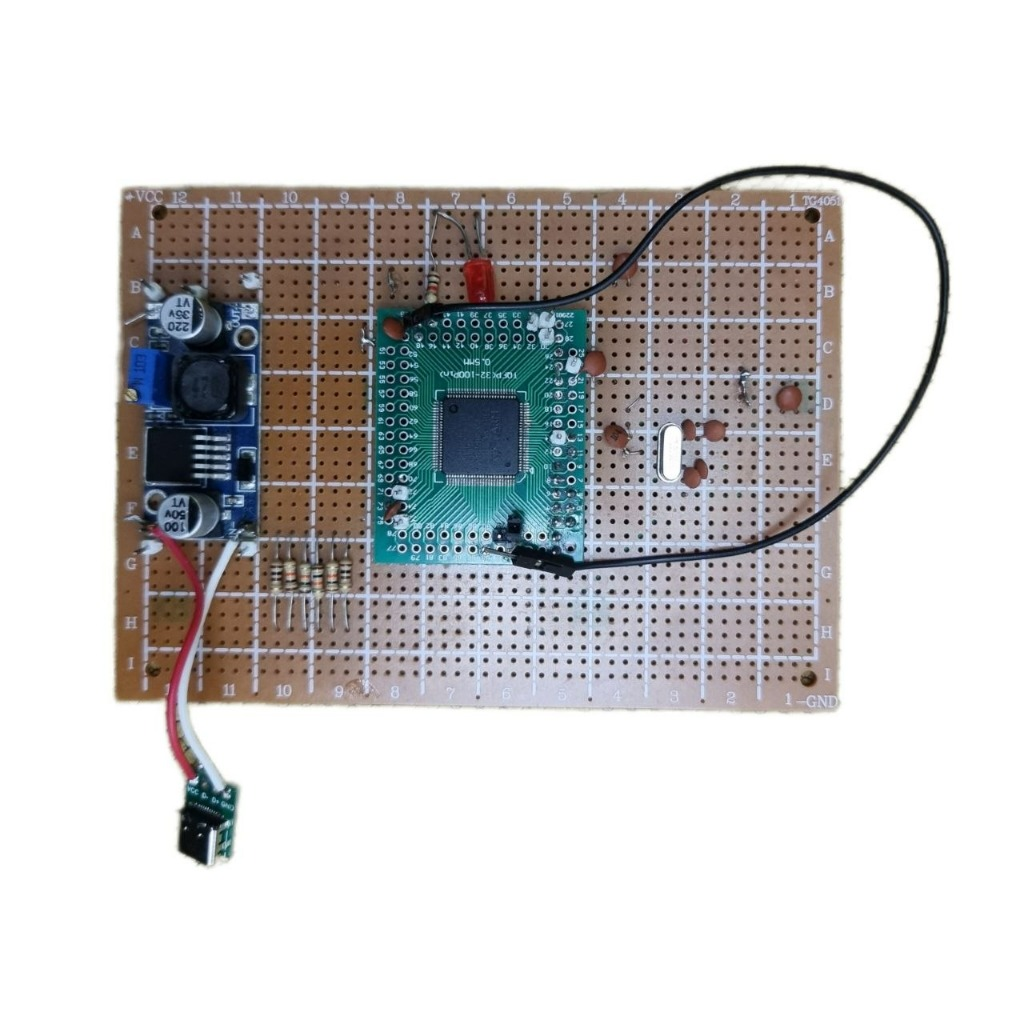
\includegraphics[height=5.2cm, keepaspectratio]{figures/board_handmade_perfboard.jpg}
\caption{هدربرد دست‌ساز اولیه پیاده‌سازی‌شده بر روی برد هزارسوراخ}
\label{fig:board_handmade}
\end{figure}

\section{گذار به هدربرد تجاری \lr{STM32H750VBT6} و مشخصات فنی آن}
\label{sec:commercial_board_transition}
با گذر زمان و پیگیری‌های مستمر، یک هدربرد ساده و استاندارد تجاری از میکروکنترلر \lr{STM32H750VBT6} در بازار داخلی موجود شد و بلافاصله خریداری گردید. از آن پس، تمامی فرآیندهای توسعه نرم‌افزاری و سخت‌افزاری بر روی این هدربرد هدایت شد.

ورود هدربرد تجاری، جهش بزرگی در کیفیت و پایداری آزمایش‌ها ایجاد کرد؛ به‌طوری‌که چالش‌های پروگرم کردن تراشه، نویز خطوط \lr{Trace}، سختی اتصالات و شکنندگی مکانیکی کاملاً برطرف شده و دیگر چالشی در مسیر پروژه محسوب نمی‌شدند. شکل \ref{fig:board_commercial} هدربرد تجاری تهیه‌شده را نشان می‌دهد که دارای پکیج ۱۰۰ پایه \lr{LQFP} و جانمایی استاندارد است.

\begin{figure}[H]
\centering
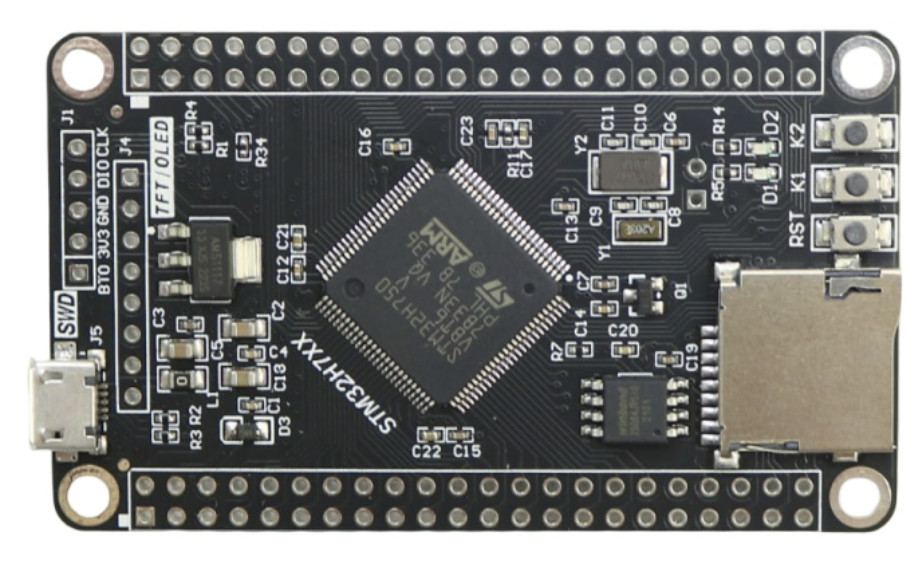
\includegraphics[height=5.5cm, keepaspectratio]{figures/board_commercial_h750.png}
\caption{هدربرد استاندارد تجاری \lr{STM32H750VBT6}}
\label{fig:board_commercial}
\end{figure}

\subsection{تخصیص پایه‌ها و مسیرکشی اختصاصی \lr{Trace}}
پایه‌های ردیابی موازی ۴ بیتی در تراشه \lr{STM32H750} بر روی پورت \lr{E} قرار دارند. جدول \ref{tab:tpiu_pins} مشخصات سیگنال‌ها و جانمایی پایه‌ها را به همراه خط‌کشی کامل نمایش می‌دهد:

\begin{table}[ht]
\centering
\caption{تخصیص پایه‌های فیزیکی میکروکنترلر \lr{STM32H750VBT6} به درگاه \lr{TPIU}}
\label{tab:tpiu_pins}
\begin{tabularx}{\textwidth}{|l|c|c|c|X|}
\hline
\textbf{پایه تراشه} & \textbf{شماره پین} & \textbf{سیگنال \lr{TPIU}} & \textbf{تابع جایگزین} & \textbf{پیکربندی درگاه} \\
\hline
\texttt{PE2} & پین ۱ & \texttt{TRACECLK} & \lr{AF0} & \lr{Very High Speed (100MHz+)} \\
\hline
\texttt{PE3} & پین ۲ & \texttt{TRACED0} & \lr{AF0} & \lr{Very High Speed (100MHz+)} \\
\hline
\texttt{PE4} & پین ۳ & \texttt{TRACED1} & \lr{AF0} & \lr{Very High Speed (100MHz+)} \\
\hline
\texttt{PE5} & پین ۴ & \texttt{TRACED2} & \lr{AF0} & \lr{Very High Speed (100MHz+)} \\
\hline
\texttt{PE6} & پین ۵ & \texttt{TRACED3} & \lr{AF0} & \lr{Very High Speed (100MHz+)} \\
\hline
\end{tabularx}
\end{table}

یکی از مزایای مهم فیزیکی پکیج \lr{LQFP100} در این تراشه، مجاورت پایه‌های ۱ تا ۵ با یکدیگر در گوشه سمت چپ بالای آی‌سی است. این امر باعث می‌شود که خطوط کلاک و داده ردیابی در کمترین فاصله ممکن به پین‌هدرهای لبه برد برسند و تطبیق طول مسیرها با کمترین اختلاف فاز ممکن میسر گردد.

\subsection{ملاحظات دی‌کوپلینگ و پایداری تغذیه}
تغییر وضعیت همزمان ۵ پین دیجیتال در فرکانس بالا با نرخ تغییر ولتاژ حداکثری، جریانی لحظه‌ای به ریل‌های تغذیه وارد می‌کند. در هدربرد تجاری خریداری‌شده، وجود صفحه زمین پیوسته و خازن‌های سرامیکی \lr{100nF} چندلایه (\lr{MLCC}) در نزدیکی پایه‌های \texttt{VDD/VSS}، پدیده جهش زمین را به حداقل رسانده و مسیر برگشت جریان را با کمترین اندوکتانس حلقه مسدود ساخته است.

\section{یکپارچگی سیگنال در کابل‌های رابط و پروب‌ها}
برای انتقال سیگنال‌ها از هدربرد به ابزار دریافت لاجیک، اصول یکپارچگی سیگنال مد نظر قرار گرفت:
\begin{enumerate}
    \item \textbf{طول کابل‌های اتصال:} استفاده از کابل‌های بلند رابط به دلیل ایجاد اندوکتانس پارازیتی موجب نوسانات پله‌ای (\lr{Ringing}) و خوانش اشتباه سطوح منطقی می‌گردد. بنابراین، طول کابل‌های پروب به کمتر از ۱۰ سانتی‌متر محدود گردید.
    \item \textbf{تنظیم ثبّات نرخ خیز خروجی (\lr{OSPEEDR}):} ثبّات \lr{GPIOE\_OSPEEDR} برای تمام پایه‌های \texttt{PE2..PE6} بر روی وضعیت «سرعت بسیار بالا» (\lr{0b11 - Very High Speed}) تنظیم شد تا زمان خیز و افت پالس‌ها به حداقل رسیده و لبه‌های کلاک به صورت کاملاً شارپ شکل گیرند.
\end{enumerate}

\section{معماری سمپلینگ با فرکانس متناسب (سمپلینگ ۱۰ برابری)}
\label{sec:sampling_strategy}
در سامانه‌های صنعتی مجهز به پروب‌های سخت‌افزاری پیشرفته، دیباگر مستقیماً با کلاک سنکرون تراشه در فرکانس‌های ۱۰۰ مگاهرتز به بالا هماهنگ می‌شود. اما در سناریوی استفاده از لاجیک‌آنالایزرهای عمومی اقتصادی، این رویکرد به دلیل تغییرات فاز کلاک و عدم تطبیق زمان برپایی و نگه‌داری (\lr{Setup \& Hold Time}) منجر به پرش بیت‌ها می‌گردد. برای دستیابی به اطمینان ۱۰۰ درصدی، استراتژی سمپلینگ ناهمگام با نرخ متناسب ۱۰ برابری اتخاذ گردید.

\subsection{مشخصات لاجیک‌آنالایزر \lr{DSLogic U3Pro16}}
\label{sec:dslogic_hw}
برای ثبت سیگنال‌های درگاه ردیابی، از لاجیک‌آنالایزر پرسرعت \lr{DSLogic U3Pro16} ساخت شرکت \lr{DreamSourceLab} استفاده شد. این دستگاه دارای ۱۶ کانال ورودی دیجیتال، ارتباط پرسرعت \lr{USB 3.0} و حافظه داخلی \lr{2Gb DDR3 DRAM} است که امکان نمونه‌برداری با فرکانس‌های بالا را بدون افت فریم در بافر داخلی فراهم می‌کند. شکل \ref{fig:dslogic_hardware} این دستگاه را نمایش می‌دهد.

\begin{figure}[ht]
\centering
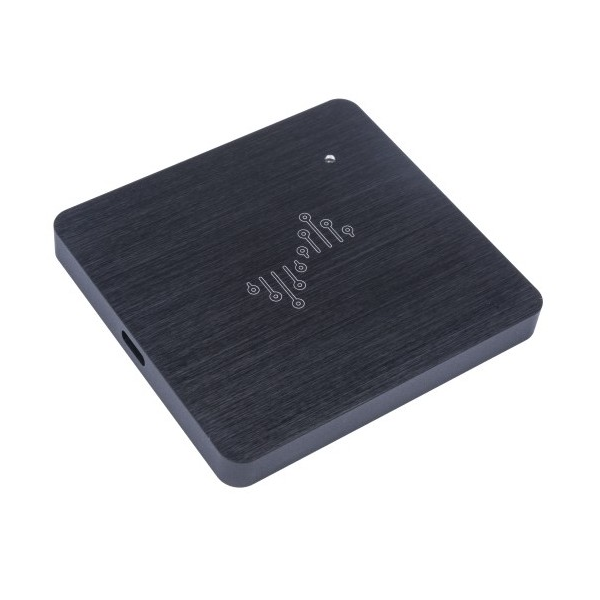
\includegraphics[width=0.62\textwidth]{figures/dslogic_u3pro16.png}
\caption{لاجیک‌آنالایزر سخت‌افزاری \lr{DSLogic U3Pro16} با رابط پرسرعت \lr{USB 3.0} و حافظه داخلی \lr{DRAM}}
\label{fig:dslogic_hardware}
\end{figure}

\subsection{استراتژی سمپلینگ ۱۰ برابری و استخراج پایدار داده‌ها}
\label{sec:sampling_technique}
برای تضمین دریافت بیست‌درصدی داده‌ها و حذف کامل خطای فاز:
\begin{itemize}
    \item کلاک پردازنده و کلاک خروجی درگاه ردیابی در یک پله کاری پایدار (مانند ۱۰ مگاهرتز یا کلاک مقیاس‌شده ۱ مگاهرتز) تنظیم می‌گردد.
    \item لاجیک‌آنالایزر با نرخ نمونه‌برداری \textbf{۱۰ برابری} (به عنوان مثال ۱۰۰ مگاهرتز برای کلاک ردیابی ۱۰ مگاهرتز) خطوط \texttt{TRACECLK} و \texttt{TRACED[0:3]} را اسکن می‌نماید.
\end{itemize}

همان‌طور که در شکل \ref{fig:sampling_concept} مشاهده می‌شود، سمپلینگ با ضریب ۱۰ برابری مزایای بنیادینی به همراه دارد:
\begin{enumerate}
    \item هر نیم‌پریود کلاک شامل حداقل ۵ نمونه دیجیتال است؛ بنابراین نرم‌افزار میزبان لبه‌های بالارونده و پایین‌رونده را بدون تأثیرپذیری از نویزهای ضربه‌ای تک‌نمونه‌ای شناسایی می‌کند.
    \item خطوط داده (\lr{TRACED[0:3]}) در نمونه میانی (نمونه سوم در پنجره ۵ نمونه‌ای) خوانده می‌شوند؛ یعنی دقیقاً در مرکز چشم‌پالس الکتریکی (\lr{Eye Diagram}) که سیگنال به بیشترین ثبات ولتاژی رسیده و زمان‌های برپایی و نگه‌داری کاملاً ارضا شده‌اند.
\end{enumerate}

\begin{figure}[ht]
\centering
\begin{latin}
\begin{tikzpicture}[xscale=0.78, yscale=0.9]
    % Clock wave
    \draw[thick, black] (0,2) -- (2,2) -- (2,0) -- (4,0) -- (4,2) -- (6,2) -- (6,0) -- (8,0) -- (8,2) -- (10,2);
    \node[left] at (0,1) {\texttt{TRACECLK}};
    
    % Data wave
    \draw[thick, blue] (0,0.5) -- (1.8,0.5) -- (2.2,1.5) -- (5.8,1.5) -- (6.2,0.5) -- (10,0.5);
    \node[left] at (0,-0.5) {\texttt{TRACED[0:3]}};
    \node[blue] at (4,1.0) {\small \rl{نیبل معتبر} (Nibble Data)};
    
    % Sampling ticks (10x sampling)
    \foreach \x in {0.2, 0.6, 1.0, 1.4, 1.8, 2.2, 2.6, 3.0, 3.4, 3.8, 4.2, 4.6, 5.0, 5.4, 5.8, 6.2, 6.6, 7.0, 7.4, 7.8, 8.2, 8.6, 9.0, 9.4, 9.8} {
        \draw[red!70, dashed] (\x, -1.0) -- (\x, 2.3);
        \fill[red] (\x, -1.0) circle (1.5pt);
    }
    \node[right, red!80!black] at (10,-1.0) {\small \rl{نمونه‌های ۱۰ برابری} (10x Samples)};
    
    % Optimal sampling point
    \draw[latex-, very thick, green!50!black] (3.0,1.55) -- (3.0,2.6) node[above, font=\small, text=green!50!black] {\rl{نقطه پایدار نمونه‌برداری در مرکز چشم}};
\end{tikzpicture}
\end{latin}
\caption{نمودار زمانی تکنیک سمپلینگ ۱۰ برابری و استخراج پایدار داده‌ها در مرکز چشم الکتریکی}
\label{fig:sampling_concept}
\end{figure}

\subsection[مشاهدات تجربی دیوتی‌سایکل و کوانتیزاسیون]{مشاهدات تجربی دیوتی‌سایکل و توجیه تئوری کوانتیزاسیون دیجیتال}
\label{sec:duty_cycle_quantization}
در مراحل اولیه آزمایش‌های عملی، پدیده‌ای جالب توجه در ثبت سیگنال کلاک \lr{Trace} مشاهده شد: هنگامی که یک سیگنال کلاک با فرکانس اسمی ۱۰ مگاهرتز (پریود ۱۰۰ نانوثانیه) با نرخ نمونه‌برداری ۱۰۰ مگاهرتز (۱۰ برابر فرکانس سیگنال) ثبت می‌شد، مقادیر دیوتی‌سایکل اندازه‌گیری‌شده توسط نرم‌افزار لاجیک‌آنالایزر همواره ثابت نبود. در برخی دوره‌ها، دیوتی‌سایکل دقیقاً ۵۰ درصد (\lr{50.00\%}) با عرض پالس مثبت ۵۰ نانوثانیه بود (شکل \ref{fig:dslogic_duty50})؛ اما در سایر دوره‌ها یا نمونه‌برداری‌های دیگر، این مقدار به اعدادی نظیر ۴۰ درصد (\lr{40.00\%} در شکل \ref{fig:dslogic_duty40})، ۶۰ درصد، ۵۶ درصد یا مقادیر نامتقارن دیگر تغییر می‌کرد.

\begin{figure}[ht]
\centering
\begin{subfigure}[b]{0.48\textwidth}
    \centering
    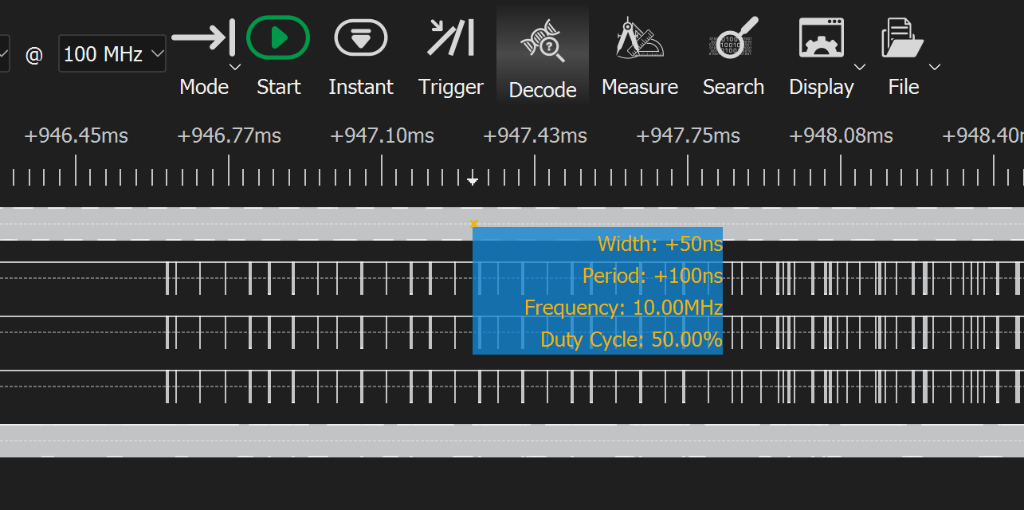
\includegraphics[width=\textwidth]{figures/dslogic_duty50.png}
    \caption{نمونه‌برداری با دیوتی‌سایکل متقارن ۵۰ درصد (\lr{Width: +50ns})}
    \label{fig:dslogic_duty50}
\end{subfigure}
\hfill
\begin{subfigure}[b]{0.48\textwidth}
    \centering
    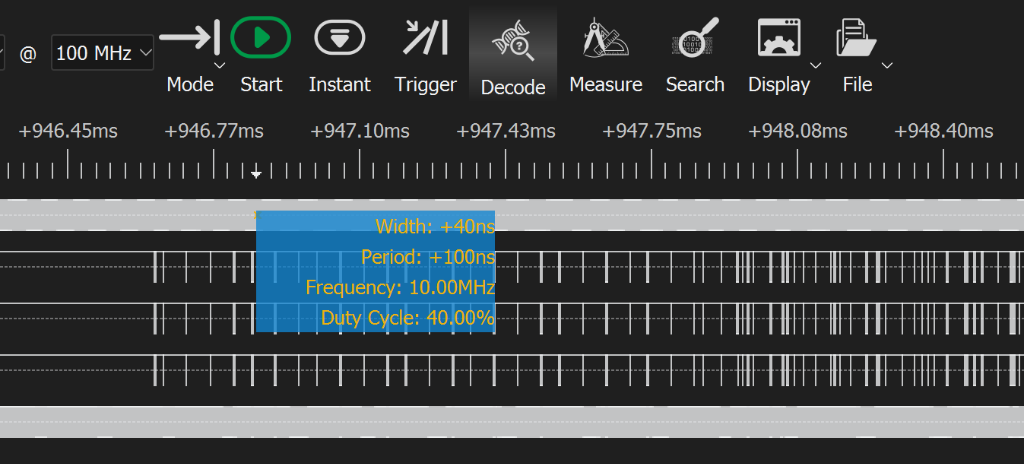
\includegraphics[width=\textwidth]{figures/dslogic_duty40.png}
    \caption{نمونه‌برداری با دیوتی‌سایکل نامتقارن ۴۰ درصد (\lr{Width: +40ns})}
    \label{fig:dslogic_duty40}
\end{subfigure}
\caption{مشاهدات تجربی اندازه‌گیری کلاک \lr{Trace} ۱۰ مگاهرتز توسط لاجیک‌آنالایزر در نرخ نمونه‌برداری ۱۰۰ مگاهرتز}
\label{fig:dslogic_duty_comparison}
\end{figure}

با بررسی دقیق فرآیند نمونه‌برداری لاجیک‌آنالایزر و مراجعه به راهنمای کاربری سازنده (\lr{DreamSourceLab DSView User Guide}) \cite{dslab2023dsview}، مشخص گردید که این نوسان دیوتی‌سایکل ناشی از \textbf{طبیعت دیجیتال و ناهمگام نمونه‌برداری گسسته در زمان} (\lr{Asynchronous Discrete-Time Quantization}) است و نشان‌دهنده تغییر فیزیکی در سیگنال خروجی میکروکنترلر نیست. دلایل تئوری این رخداد به شرح زیر تبیین می‌گردد:
\begin{enumerate}
    \item \textbf{خطای کوانتیزاسیون زمانی (\lr{Timing Quantization Uncertainty}):} لاجیک‌آنالایزر مجهز به اسیلاتور محلی خود است که مستقل از کلاک میکروکنترلر عمل می‌کند. در نرخ نمونه‌برداری ۱۰۰ مگاهرتز، فاصله زمانی بین دو نمونه متوالی $T_s = 10\,\mathrm{ns}$ است. از آنجا که لبه واقعی پالس کلاک می‌تواند در هر نقطه‌ای میان دو تیک نمونه‌برداری رخ دهد، بر اساس اصل نمونه‌برداری دیجیتال، عدم قطعیت در تشخیص هر لبه معادل $\pm T_s$ یعنی $\pm 10\,\mathrm{ns}$ خواهد بود \cite{dslab2023dsview}.
    \item \textbf{توزیع نمونه‌ها در یک دوره پریودیک:} در یک دوره تناوب ۱۰۰ نانوثانیه‌ای، دقیقاً ۱۰ نمونه ثبت می‌شود. اگر فاز کلاک نمونه‌برداری به‌طور متقارن با سیگنال ورودی قفل شده باشد، ۵ نمونه در سطح بالا (\lr{High}) و ۵ نمونه در سطح پایین (\lr{Low}) قرار می‌گیرند که دیوتی‌سایکل را ۵۰ درصد نشان می‌دهد ($5 \times 10\,\mathrm{ns} = 50\,\mathrm{ns}$). اما یک جابجایی زمانی ناچیز، لغزش فاز یا جیتر به میزان چند نانوثانیه کافی است تا یکی از نمونه‌های نزدیک به لبه تغییر وضعیت داده و تعداد نمونه‌های سطح بالا به ۴ و سطح پایین به ۶ برسد؛ در نتیجه دیوتی‌سایکل اندازه‌گیری‌شده برابر ۴۰ درصد ($4 \times 10\,\mathrm{ns} = 40\,\mathrm{ns}$) گزارش می‌شود.
    \item \textbf{توجیه نیاز به سمپلینگ ۱۰ برابری بر پایه مستندات سازنده:} در راهنمای رسمی لاجیک‌آنالایزر \cite[بخش ۲.۳.۲ و شکل ۲-۱۰]{dslab2023dsview} صراحتاً بیان شده است که با ضریب نمونه‌برداری کمتر (نظیر ۲ یا ۵ برابر)، خطای زمانی به $1/2 T$ یا $1/5 T$ می‌رسد که می‌تواند به از دست رفتن کامل پالس‌ها (\lr{Pulse Loss}) یا اعوجاج شدید دیوتی‌سایکل (نظیر نسبت‌های ۳ به ۲ یا ۵ به ۳) منجر شود. در مقابل، سمپلینگ با ضریب ۱۰ برابری خطای فاز را به کمتر از ۱۰ درصد ($\pm 10\%$) محدود کرده و تضمین می‌نماید که تمامی لبه‌ها بدون پرش بیت شناسایی شوند. این تطابق کامل مشاهدات تجربی با روابط تئوری کوانتیزاسیون، مهر تأییدی بر کفایت و ضرورت ضریب ۱۰ برابری در این سامانه بود.
\end{enumerate}

\section{بررسی و دلایل رد درگاه \lr{Serial Wire} جهت دریافت \lr{Trace}}
\label{sec:rejection_of_swo}
در مراحل طراحی معماری سخت‌افزاری سامانه، این پرسش مطرح شد که آیا می‌توان به جای درگاه موازی چندسیمه \lr{TPIU}، داده‌های ردیابی را بر روی درگاه سریال \lr{Serial Wire (SW / SWO)} دریافت نمود تا از چالش‌های سیم‌کشی متعدد، ملاحظات فرکانس بالا و نیاز به لاجیک‌آنالایزر چندکاناله رهایی یافت؟ با ارزیابی دقیق معماری پردازنده و الزامات آزمون، این گزینه به دلایل قاطع زیر رد گردید:
\begin{enumerate}
    \item \textbf{پهنای باند بسیار بالای داده‌های \lr{Trace} دستورات (\lr{High Bandwidth of ETM Trace}):} ماژول ردیابی دستورات (\lr{ETMv4}) به ازای هر انشعاب برنامه، استثنا یا تغییر مسیر کنترلی، بسته‌های ردیابی اتم (\lr{Atom Packets}) و نشانی هدف تولید می‌کند. در پردازنده‌های مدرن فرکانس بالا، حجم این داده‌ها به ده‌ها مگابایت بر ثانیه می‌رسد. خط تک‌سیمه \lr{SWO} که در مدهای آسنکرون \lr{UART} یا منچستر کار می‌کند، دارای پهنای باند بسیار محدودی (معمولاً در محدوده چند مگابیت بر ثانیه) است و به سرعت دچار سرریز بافر و افت بسته‌ها (\lr{Packet Loss}) می‌گردد.
    \item \textbf{عدم وجود یا محدودیت بافر اختصاصی \lr{Trace} در تراشه (\lr{Lack of Trace Buffer}):} بسیاری از میکروکنترلرهای سری استاندارد (از جمله \lr{STM32H750}) فاقد بافرهای حجیم آن‌چیپ نظیر \lr{Embedded Trace Buffer (ETB)} یا \lr{Embedded Trace FIFO (ETF)} هستند تا بتوانند جریان کامل \lr{Trace} را در حافظه درونی متوقف و سپس به صورت قطره‌چکانی تخلیه کنند. بنابراین، داده‌های \lr{Trace} باید به صورت کاملاً بی‌درنگ و با کمترین تأخیر به دنیای خارج هدایت شوند که تنها از عهده درگاه موازی پرسرعت برمی‌آید.
    \item \textbf{اشغال انحصاری درگاه \lr{SW} توسط پروژه مکمل برای تبادل ورودی/خروجی:} حیاتی‌ترین دلیل رد این گزینه، وابستگی معماری کلان سامانه آزمون به درگاه \lr{SWD} بود. در این ساختار مشترک، پورت \lr{SW} (شامل پایه‌های \texttt{SWDIO} و \texttt{SWCLK}) به‌طور مداوم توسط پروژه مکمل جهت تزریق تحریک‌های تست (\lr{Test Stimuli}) به داخل ثبّات‌ها و خواندن مقادیر ورودی/خروجی و پاسخ‌های سخت‌افزار تحت آزمون استفاده می‌شد. اشغال این درگاه برای داده‌های حجیم ردیابی، به مسدود شدن کانال آزمون و بن‌بست ارتباطی منجر می‌گردید.
    \item \textbf{فقدان کلاک فیزیکی سنکرون و ناسازگاری با استاندارد \lr{Trace} دستورات:} پایه \lr{SWO} فاقد کلاک سنکرون فیزیکی (\texttt{TRACECLK}) است و در سطح سخت‌افزار تنها برای ارسال بسته‌های رویدادی ماژول‌های سبک‌تر نظیر \lr{ITM} (\lr{Instrumentation Trace}) و \lr{DWT} طراحی شده است؛ در حالی که ردیابی چرخه‌دقیق دستورات نیازمند گذرگاه همگام چندبیتی \lr{TPIU} با تضمین هم‌زمانی کلاک و داده است.
\end{enumerate}

بنابراین، پیاده‌سازی سخت‌افزاری مبتنی بر درگاه ۴ بیتی موازی \lr{TPIU} به همراه کلاک اختصاصی، تنها رویکرد ممکن و استاندارد برای دستیابی به ردیابی کامل و بی‌درنگ دستورات بدون تداخل با فرآیند آزمون نرم‌افزار ارزیابی گردید.

\section{جمع‌بندی فصل}
در این فصل، مسیر تکامل بستر سخت‌افزاری سامانه از هدربرد دست‌ساز اولیه ساخته‌شده بر روی برد هزارسوراخ تا گذار موفق به هدربرد استاندارد تجاری \lr{STM32H750VBT6} تبیین گردید. تمهیدات یکپارچگی سیگنال شامل کوتاه نگاه داشتن طول پروب‌ها و تنظیم خروجی‌های سرعت بسیار بالا شرح داده شد. سپس معماری سمپلینگ ۱۰ برابری با استفاده از لاجیک‌آنالایزر \lr{DSLogic U3Pro16} معرفی شد و پدیده تجربی تغییر دیوتی‌سایکل بر پایه تئوری کوانتیزاسیون دیجیتال ناهمگام و استانداردهای سازنده لاجیک‌آنالایزر توجیه گردید. در نهایت، دلایل فنی و عملیاتی رد درگاه \lr{Serial Wire} به نفع درگاه موازی \lr{TPIU} بررسی شد. در فصل پنجم، پیکربندی سطح پایین ثبّات‌های درونی میکروکنترلر و \lr{Firmware} مورد نیاز جهت فعال‌سازی این بستر سخت‌افزاری تشریح خواهد شد.


% فصل پنجم: پیکربندی ETMv4 و Firmware
% ==============================================================================
% فصل پنجم: پیکربندی ETMv4 و پیاده‌سازی Firmware
% ==============================================================================

\chapter{پیکربندی \lr{ETMv4} و پیاده‌سازی \lr{Firmware}}
\label{ch:firmware}

\section{مقدمه}
زیرسیستم ردیابی و عیب‌یابی \lr{CoreSight} در میکروکنترلرهای پیشرفته مبتنی بر معماری \lr{ARM Cortex-M7} (نظیر \lr{STM32H750})، مجموعه‌ای بسیار غنی از ماژول‌های مستقل سیلیکونی است که در فضای نگاشت‌شده حافظه (\lr{Memory-Mapped I/O}) قرار دارند. این ماژول‌ها پس از روشن شدن اولیه تراشه، به منظور جلوگیری از مصرف بیهوده توان و ممانعت از ایجاد تداخل‌های ناخواسته بر خطوط کلاک و پین‌های خروجی، در وضعیت کاملاً قفل‌شده و خاموش قرار دارند. راه‌اندازی این زیرسیستم بدون نقض شرط بنیادین «غیرتهاجمی بودن» (\lr{Non-Intrusiveness}) و بدون اعمال هرگونه اثر جانبی بر فرکانس و رفتار زمانی برنامه‌های کاربر، نیازمند مهندسی دقیق ترتیب پیکربندی ثبّات‌ها، مدیریت دامنه‌های توان و کلاک، و حل چالش‌های پنهان تطبیق معماری است.

در این فصل، ابتدا پروتکل فشرده‌سازی جریان دستورات در \lr{ETMv4} تبیین می‌گردد. سپس ساختار معماری زیرساخت دیباگ، دامنه‌های توان و توزیع کلاک در \lr{STM32H750} به همراه بلوک‌دیاگرام‌های مربوطه از راهنمای مرجع شرکت سازنده تشریح می‌شود. در ادامه، نگاشت حافظه و مراحل گام‌به‌گام پیکربندی ثبّاتی با تأکید بر ثبّات حیاتی \lr{TRCCONFIGR} بررسی شده و چالش بنیادین مغایرت راهنمای مرجع آی‌سی‌ها با استاندارد معماری \lr{ARM} تبیین می‌گردد. در بخش‌های بعدی، کالبدشکافی فایل‌های درایور مستقل \lr{\texttt{ETMv4.h}} و \lr{\texttt{ETMv4.c}} و روش به‌کارگیری محصول و تزریق به کدهای کاربری ارائه شده و در نهایت، ریشه‌یابی چالش بسته‌های همگام‌سازی (\lr{A-Sync}) و آسیب‌شناسی روش سوئیچینگ متناوب مستندسازی خواهد شد.

\section{پروتکل فشرده‌سازی جریان دستورات در \lr{ETMv4}}
\label{sec:etm_compression_protocol}
پردازنده \lr{Cortex-M7} در فرکانس‌های کاری چندصد مگاهرتزی، در هر ثانیه صدها میلیون دستورالعمل را اجرا می‌کند. ارسال بی‌درنگ و کامل آدرس ۳۲ بیتی هر دستورالعمل از طریق پایه‌های فیزیکی میکروکنترلر به پهنای باندی در مقیاس چند گیگابایت بر ثانیه نیاز دارد؛ در حالی که در عمل تنها یک گذرگاه موازی بسیار محدود (شامل یک خط کلاک و ۴ خط داده) در دسترس قرار دارد.

برای غلبه بر این محدودیت فیزیکی، استاندارد معماری \lr{ETMv4} شرکت \lr{ARM} از پروتکل فشرده‌سازی پیشرفته‌ای بر مبنای تفکیک رفتارهای خطی و غیرخطی پردازنده بهره می‌برد \cite{armetmv42017}:
\begin{enumerate}
    \item \textbf{ردیابی خطی و حذف آدرس‌ها:} تا زمانی که برنامه به صورت ترتیبی و بدون انشعاب دستورات متوالی حافظه را اجرا می‌کند، هیچ داده‌ای روی خط ردیابی ارسال نمی‌شود. دلیل این امر آن است که موتور دکودر نرم‌افزاری بر روی کامپیوتر میزبان، نسخه کامپایل‌شده باینری برنامه (\lr{.elf}) را در اختیار دارد؛ بنابراین با در دست داشتن آدرس اولیه، می‌تواند با دیس‌اسمبل کردن کد، نشانی دستورهای متوالی بعدی را خودش به صورت آفلاین محاسبه نماید.
    \item \textbf{بسته‌های انشعاب شرطی (\lr{Atom Packets}):} هنگامی که پردازنده به یک انشعاب شرطی (مانند دستورات \lr{\texttt{BEQ}}، \lr{\texttt{BNE}} یا عبارات \lr{if-else}) می‌رسد، ماژول \lr{ETM} تنها یک بیت وضعیت تولید می‌کند:
    \begin{itemize}
        \item کد \lr{E (Executed / Taken)}: نشان‌دهنده تحقق شرط و پرش به نشانی مقصد انشعاب.
        \item کد \lr{N (Not-Executed / Not-Taken)}: نشان‌دهنده عدم تحقق شرط و ادامه مسیر خطی برنامه.
    \end{itemize}
    سخت‌افزار \lr{ETM} جهت بیشینه‌سازی فشرده‌سازی، چندین اتم متوالی را در قالب یک بایت تجمیع کرده و به صورت بسته‌های تک‌بایتی به خروجی می‌فرستد.
    \item \textbf{بسته‌های همگام‌سازی (\lr{I\_SYNC} و \lr{A-Sync}):} به منظور بازیابی نقطه شروع اجرای برنامه یا هدایت دکودر در هنگام پرش‌های غیرمستقیم (نظیر فراخوانی توابع از طریق اشاره‌گرها، بازگشت از توابع یا ورود به توابع سرویس وقفه)، بسته‌های همگام‌سازی اجباری حاوی نشانی ۳۲ بیتی کامل ثبّات \lr{PC}، اطلاعات کانتکست و وضعیت کاری پردازنده ارسال می‌شوند.
    \item \textbf{برچسب‌های زمانی سخت‌افزاری (\lr{Timestamping}):} برای ارزیابی دقیق زمان سپری‌شده و همبسته‌سازی زمانی رویدادها، ماژول \lr{ETM} قادر است بسته‌های برچسب زمانی ۶۴ بیتی سراسری تولید کند.
    \item \textbf{شمارش چرخه‌های پردازنده (\lr{Cycle Counting - CCI}):} در کاربردهای تخمین بدترین زمان اجرا (\lr{WCET})، ثبت دقیق سیکل‌های سپری‌شده پردازنده بین دستورات حیاتی است. قابلیت \lr{CCI} با درج دلتای سیکل‌ها در جریان دستورات پایه، اندازه‌گیری چرخه-دقیق را بدون هیچ‌گونه سربار نرم‌افزاری فراهم می‌سازد.
\end{enumerate}

\section{معماری زیرساخت دیباگ، دامنه‌های توان و توزیع کلاک در \lr{STM32H750}}
\label{sec:debug_infra_architecture}
میکروکنترلر \lr{STM32H750} دارای زیرساخت عیب‌یابی و ردیابی بسیار پیچیده‌ای است که در راهنمای مرجع \lr{RM0433} شرکت \lr{STMicroelectronics} به تفصیل مستند شده است \cite{st2020stm32h7}. درک ساختار ارتباطی اجزای این زیرسیستم، تفکیک دامنه‌های توان و مدیریت کلاک‌های آنها پیش‌نیاز قطعی پیکربندی موفق \lr{Firmware} محسوب می‌شود.

\subsection{بلوک‌دیاگرام زیرساخت دیباگ و مسیر سیگنال‌های ردیابی}
شکل \ref{fig:debug_block_diagram} (برگرفته از شکل ۸۲۷ راهنمای مرجع \lr{RM0433})، معماری اتصالات داخلی اجزای دیباگ را نمایش می‌دهد.
\begin{figure}[H]
    \centering
    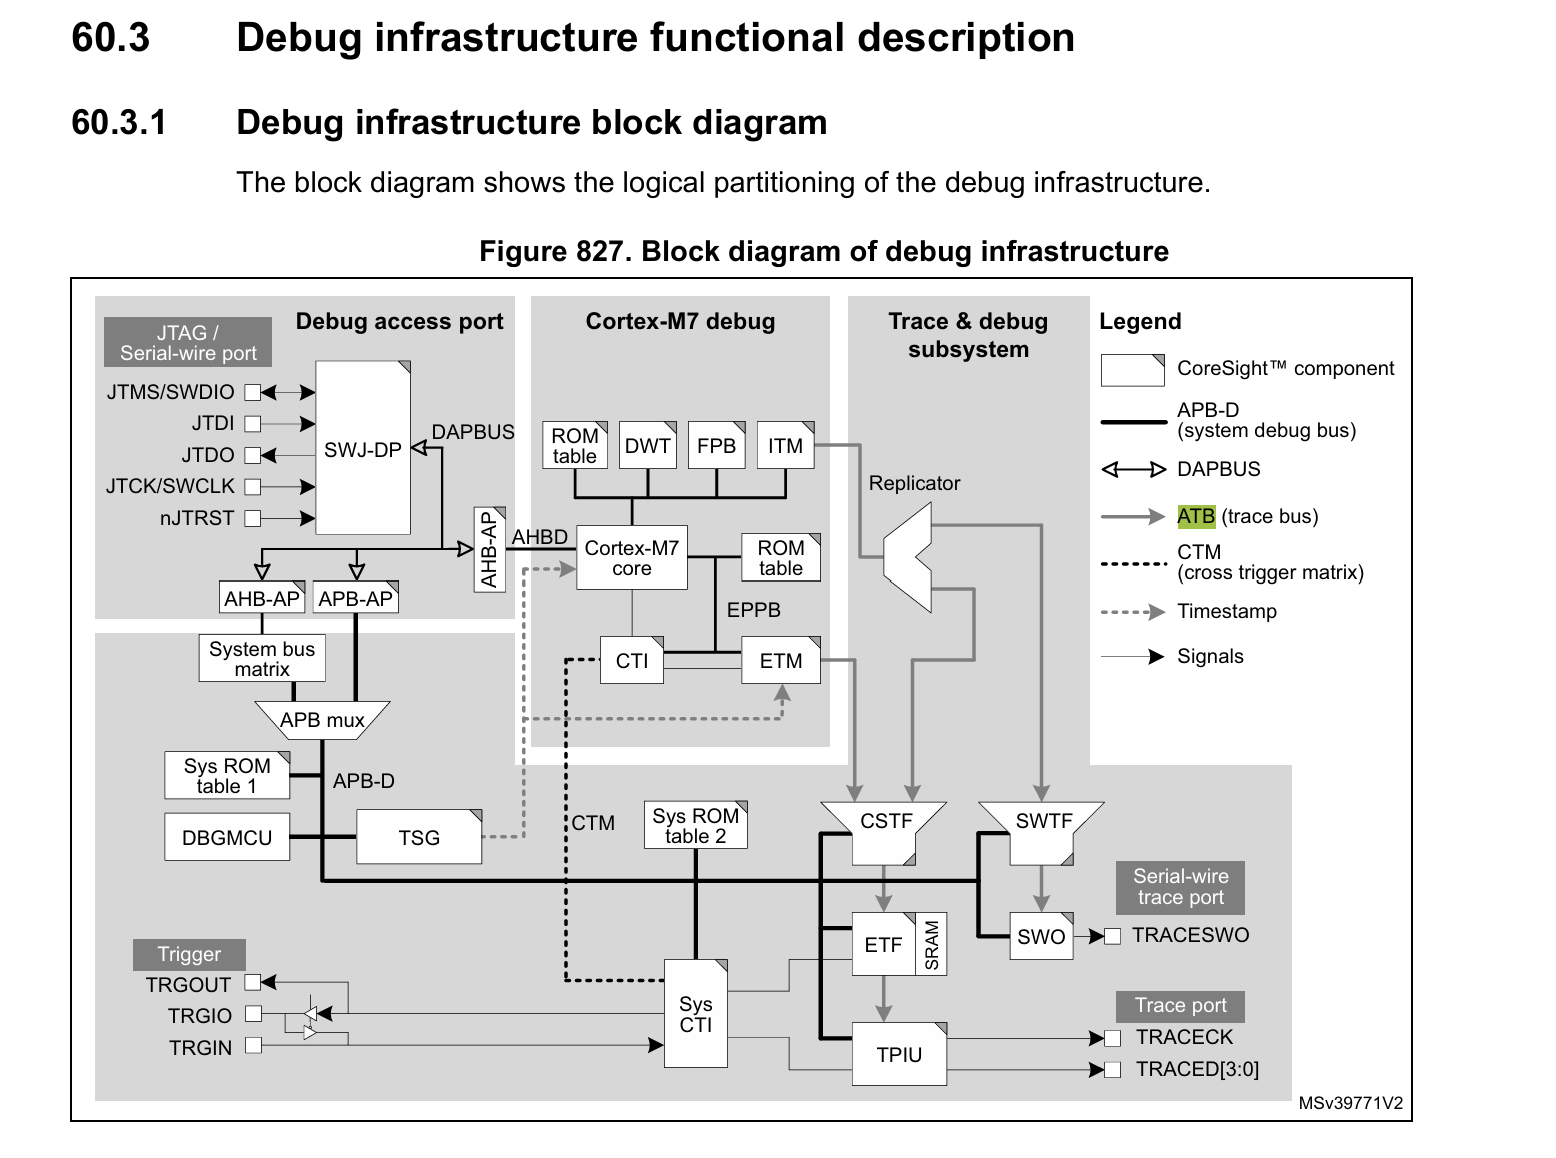
\includegraphics[width=0.88\textwidth]{figures/etm_pptx_image2.png}
    \caption{بلوک‌دیاگرام زیرساخت دیباگ و ردیابی در میکروکنترلر \lr{STM32H750} (شکل ۸۲۷  راهنمای مرجع \lr{RM0433})}
    \label{fig:debug_block_diagram}
\end{figure}

همان‌گونه که در شکل \ref{fig:debug_block_diagram} مشاهده می‌شود:
\begin{itemize}
    \item هسته پردازنده \lr{Cortex-M7} دربرگیرنده بلوک‌های \lr{ETMv4}، \lr{DWT} و \lr{ITM} است. ماژول \lr{ETMv4} پایش مستقیم گذرگاه دستورات پردازنده را بر عهده دارد.
    \item داده‌های ردیابی تولیدشده توسط \lr{ETM} و \lr{ITM} بر روی گذرگاه داخلی ۳۲ بیتی \lr{ATB (Advanced Trace Bus)} به سمت قیف ادغام ردیابی \lr{CSTF (CoreSight Trace Funnel)} هدایت می‌شوند.
    \item خروجی \lr{CSTF} وارد بافر سخت‌افزاری \lr{ETF (Embedded Trace FIFO)} می‌گردد. این بافر حافظه واسط، نوسانات شدید نرخ تولید بایت‌های \lr{Trace} در جهش‌های ناگهانی برنامه را مهار کرده و از سرریز داده‌ها جلوگیری می‌کند.
    \item در نهایت، جریان داده‌ها از خروجی \lr{ETF} وارد واحد فرمت‌بندی پورت ردیابی \lr{TPIU (Trace Port Interface Unit)} شده و این واحد، بایت‌ها را در قالب فریم‌های منظم سازمان‌دهی کرده و روی پورت موازی ۴ بیتی خارجی منتشر می‌سازد.
\end{itemize}

\subsection{دامنه‌های توان زیرساخت دیباگ (\lr{Power Domains})}
یکی از مهم‌ترین دلایل شکست تلاش‌های اولیه در راه‌اندازی ردیابی، عدم آگاهی از تفکیک دامنه‌های توان این ماژول‌ها در سیلیکون است. شکل \ref{fig:debug_power_domains} (برگرفته از شکل ۸۲۸ راهنمای مرجع \lr{RM0433}) دامنه‌های توان ماژول‌های دیباگ را تبیین می‌کند.
\begin{figure}[H]
    \centering
    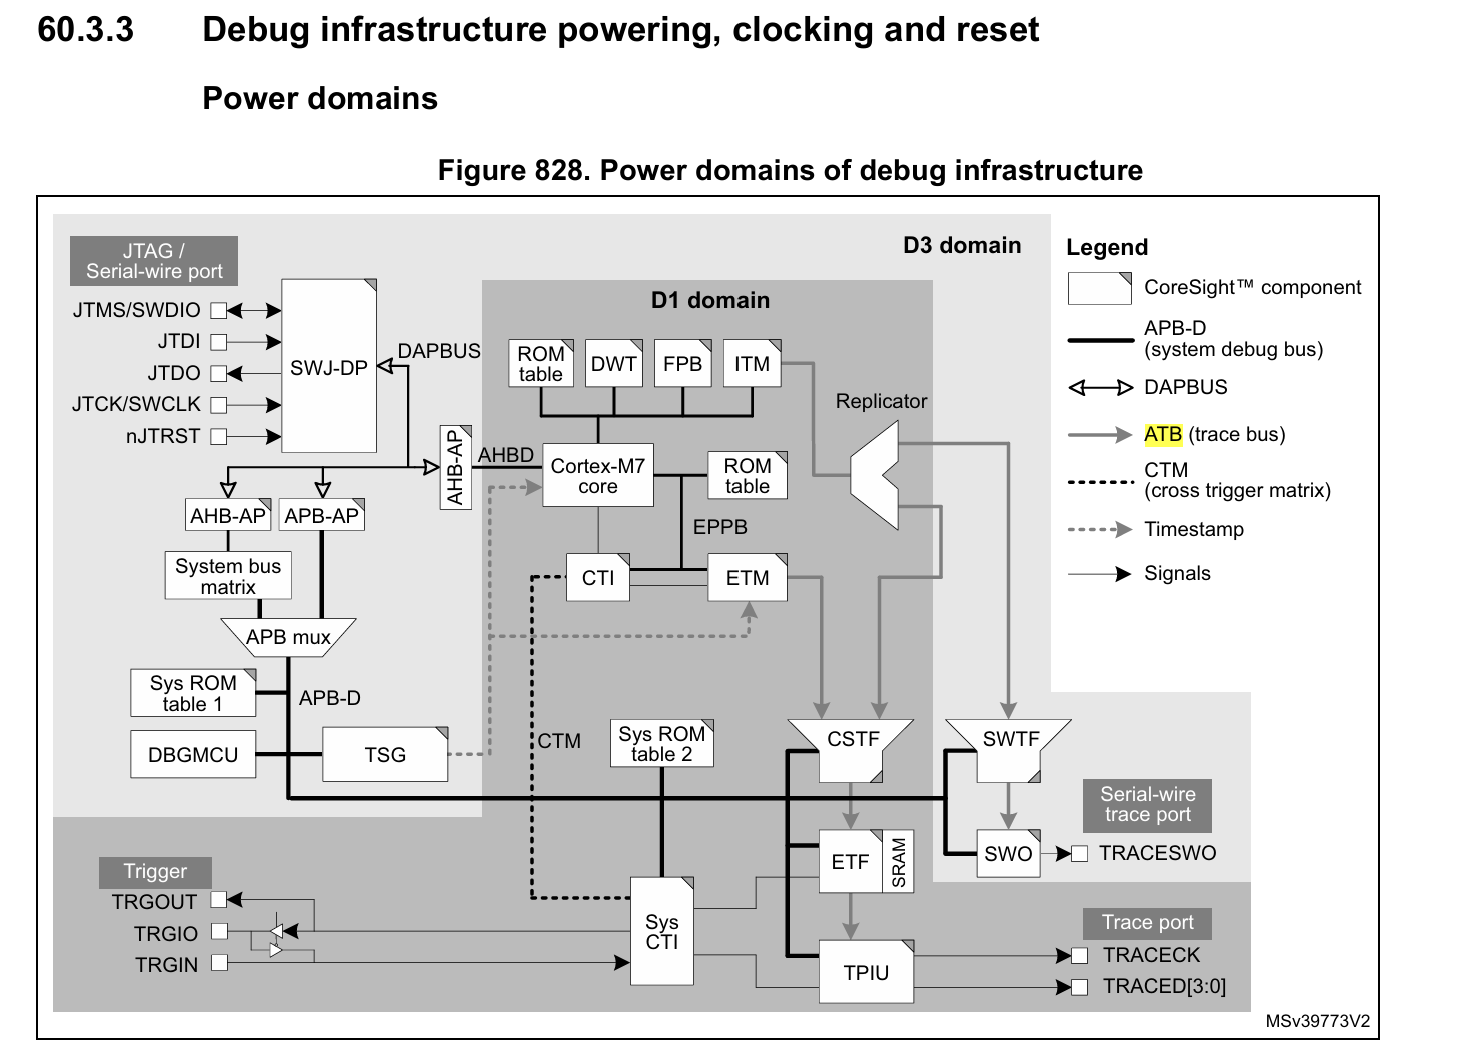
\includegraphics[width=0.85\textwidth]{figures/etm_pptx_image3.png}
    \caption{دامنه‌های توان زیرساخت دیباگ در میکروکنترلر \lr{STM32H750} (شکل ۸۲۸ راهنمای مرجع \lr{RM0433})}
    \label{fig:debug_power_domains}
\end{figure}

اجزای زیرسیستم ردیابی در دو دامنه توان متمایز قرار گرفته‌اند:
\begin{enumerate}
    \item \textbf{دامنه توان هسته (\lr{D1 Power Domain}):} هسته پردازنده \lr{Cortex-M7} و ماژول‌های محلی آن شامل \lr{ETMv4}، \lr{DWT} و \lr{ITM} در دامنه \lr{D1} قرار دارند. اگر هسته به مدهای کم‌توان (\lr{Sleep / Deep-Sleep}) وارد شود، برق این بخش قطع یا توان آن کاهش می‌یابد.
    \item \textbf{دامنه توان سیستم (\lr{D3 Power Domain}):} ماژول‌های زیرساختی شامل \lr{CSTF}، \lr{ETF}، \lr{TPIU}، \lr{DBGMCU} و درگاه \lr{SWO} در دامنه \lr{D3} قرار گرفته‌اند.
\end{enumerate}
بنابراین، \lr{Firmware} باید تضمین کند که هر دو دامنه \lr{D1} و \lr{D3} در وضعیت فعال کامل نگه داشته شوند و هیچ‌یک از اجزای مسیر ردیابی در حالت تعلیق توان قرار نگیرند.

\subsection{دامنه‌های کلاک زیرساخت دیباگ و اقدامات نرم‌افزاری}
شکل \ref{fig:debug_clock_domains} (برگرفته از شکل ۸۲۹ راهنمای مرجع \lr{RM0433}) مسیرهای توزیع کلاک را در زیرسیستم ردیابی نمایش می‌دهد.
\begin{figure}[H]
    \centering
    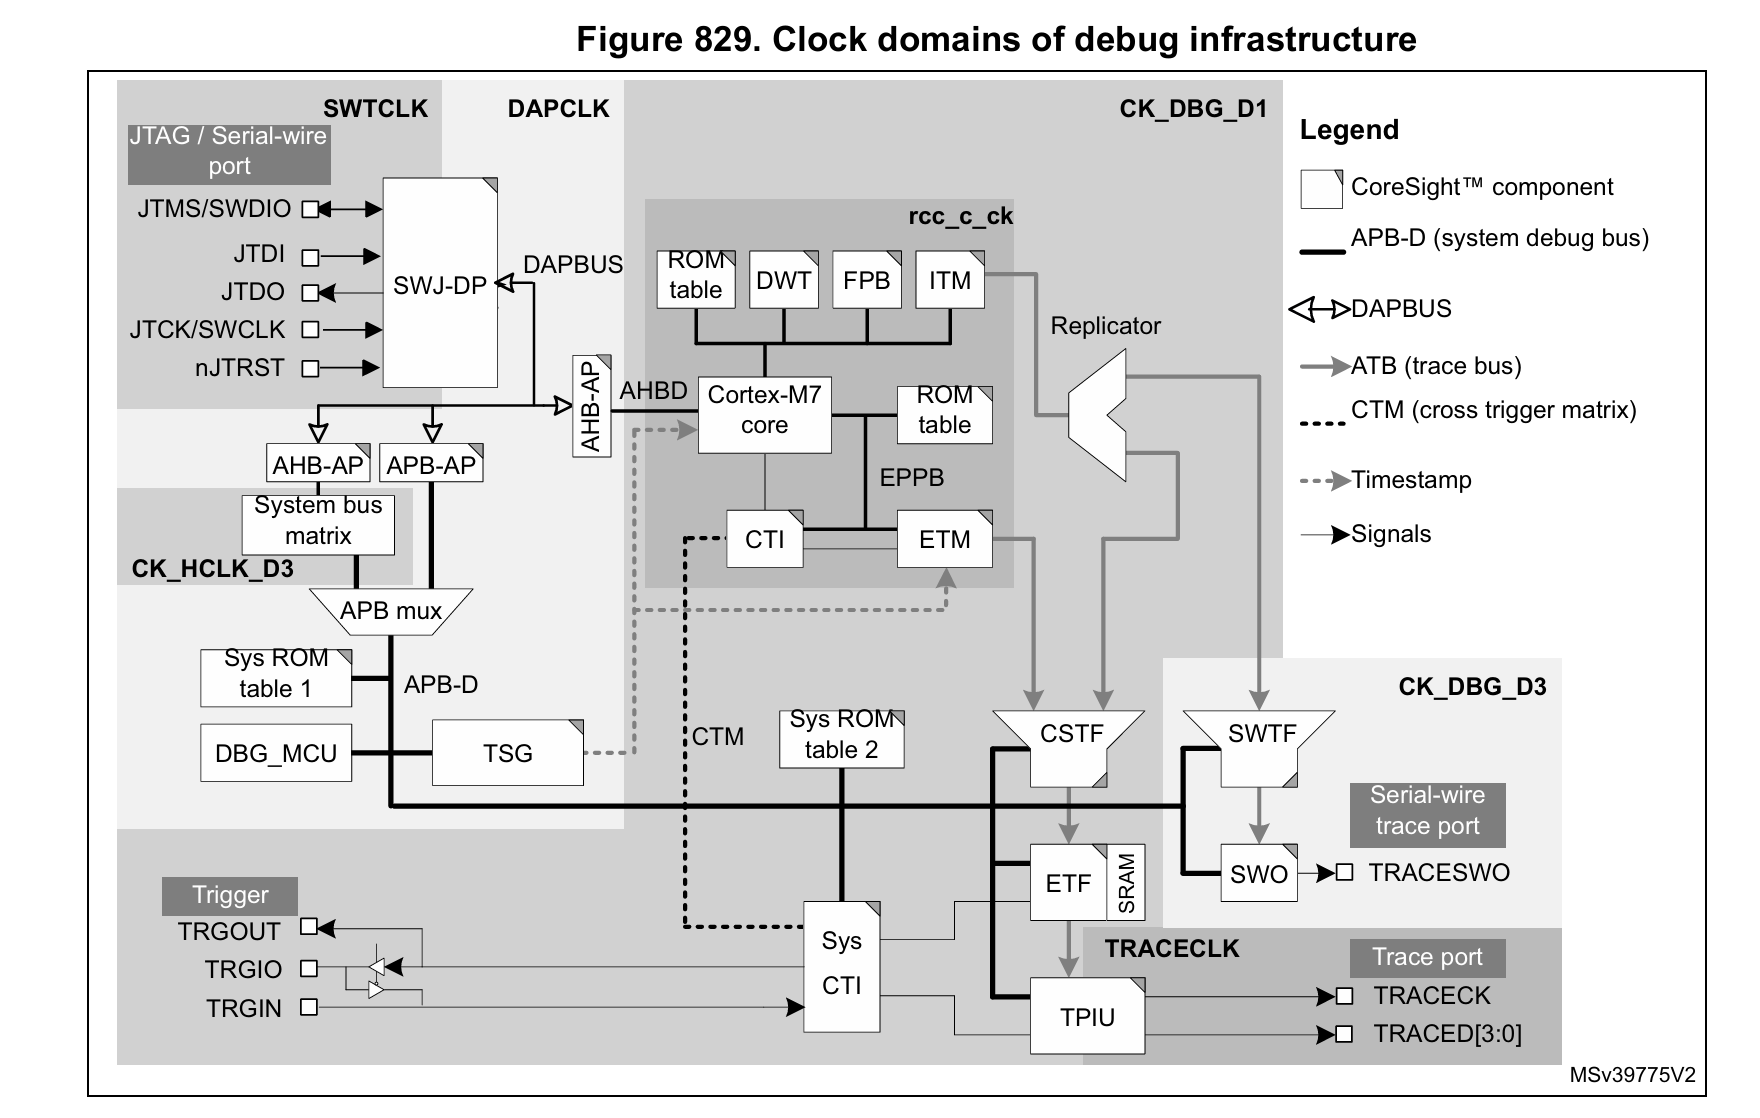
\includegraphics[width=0.88\textwidth]{figures/etm_pptx_image4.png}
    \caption{دامنه‌های کلاک زیرساخت دیباگ در میکروکنترلر \lr{STM32H750} (شکل ۸۲۹ راهنمای مرجع \lr{RM0433})}
    \label{fig:debug_clock_domains}
\end{figure}

در این ساختار، سه شبکه کلاک اساسی وجود دارد:
\begin{itemize}
    \item \textbf{کلاک هسته (\lr{CPU\_CLK}):} کلاک اصلی پردازنده که ماژول‌های \lr{ETMv4} و \lr{DWT} مستقیماً با آن کار می‌کنند. این موضوع تضمین می‌کند که ردیابی رویدادها دقیقاً با سرعت اجرای دستورات انجام می‌پذیرد.
    \item \textbf{کلاک خروجی ردیابی (\lr{TRACECLK / TRACECK}):} کلاکی که واحد \lr{TPIU} از آن برای کلاک کردن پین خروجی \lr{TRACECLK} (پایه \lr{PE2}) و تغییر وضعیت پایه‌های داده ردیابی استفاده می‌کند.
    \item \textbf{کلاک‌های گذرگاه دیباگ (\lr{DBG\_CKD1} و \lr{DBG\_CKD3}):} کلاک‌های فعال‌کننده دسترسی ثبّاتی به فضای \lr{CoreSight} در دامنه‌های \lr{D1} و \lr{D3}.
\end{itemize}

\textbf{اقدامات انجام‌شده در \lr{Firmware} جهت روشن کردن دامنه‌های کلاک و توان:}
برای فعال‌سازی کامل این مسیرها، کدهای راه‌انداز باید مراحل زیر را در ثبّات‌های سیستمی اعمال نمایند:
\begin{latin}
\begin{lstlisting}[language=C, caption={\rl{کد راه‌اندازی دامنه‌های توان و کلاک ردیابی در} \lr{DBGMCU} \rl{و} \lr{RCC}}]
/* 1. Enable GPIOE peripheral clock for trace output pins */
RCC->AHB4ENR |= RCC_AHB4ENR_GPIOEEN;

/* 2. Enable trace and debug monitor in CoreDebug */
CoreDebug->DEMCR |= CoreDebug_DEMCR_TRCENA_Msk; // Bit 24 (TRCENA = 1)

/* 3. Enable Trace clock, D1 debug clock, and D3 debug clock in DBGMCU */
DBGMCU->CR |= DBGMCU_CR_DBG_TRACECKEN | 
              DBGMCU_CR_DBG_CKD1EN     | 
              DBGMCU_CR_DBG_CKD3EN;
\end{lstlisting}
\end{latin}
بدون ست کردن همزمان بیت‌های فوق در ثبّات \lr{DBGMCU\_CR}، گذرگاه‌های \lr{ATB} و پورت \lr{TPIU} کلاک دریافت نکرده و کل سخت‌افزار ردیابی در وضعیت خاموش باقی خواهد ماند.

\section{نگاشت حافظه ثبّات‌های \lr{CoreSight} در \lr{STM32H750}}
در میکروکنترلر \lr{STM32H750}، هر یک از اجزای زیرسیستم ردیابی دارای یک بلوک آدرس ۴ کیلوبایتی در فضای دسترسی خصوصی پردازنده (\lr{Private Peripheral Bus - PPB}) یا گذرگاه \lr{AHB} هستند. جدول \ref{tab:coresight_registers} آدرس‌های پایه، دامنه‌های کاری و نقش هر مؤلفه را خلاصه نموده است \cite{st2020stm32h7}:

\begin{table}[H]
\centering
\caption{آدرس‌های پایه ماژول‌های \lr{CoreSight} در حافظه نگاشت‌شده \lr{STM32H750}}
\label{tab:coresight_registers}
\begin{tabularx}{\textwidth}{|l|c|c|X|}
\hline
\textbf{نام ماژول} & \textbf{آدرس پایه فیزیکی} & \textbf{دامنه} & \textbf{وظیفه معماری}\\
\hline
\lr{\texttt{ETMv4}} & \lr{\texttt{0xE0041000}} & \lr{PPB / D1} & موتور اصلی پایش دستورات، فشرده‌سازی شاخه‌ها و برچسب زمانی \\
\hline
\lr{\texttt{DWT}} & \lr{\texttt{0xE0001000}} & \lr{PPB / D1} & مقایسه‌گرهای آدرس، تریگرهای شروع/پایان و شمارنده چرخه \\
\hline
\lr{\texttt{DBGMCU}} & \lr{\texttt{0x5C001000}} & \lr{APB4 / D3} & کنترل کلاک‌های دیباگ، مدهای توان و فعال‌سازی \lr{Trace} \\
\hline
\lr{\texttt{TSG}} & \lr{\texttt{0x5C005000}} & \lr{AHB / D3} & تولیدکننده برچسب زمانی ۶۴ بیتی سراسری سیستم \\
\hline
\lr{\texttt{CSTF}} & \lr{\texttt{0x5C013000}} & \lr{AHB / D3} & قیف ادغام داده‌های \lr{Trace} و تخصیص شناسه جریان (\lr{Source ID}) \\
\hline
\lr{\texttt{ETF}} & \lr{\texttt{0x5C014000}} & \lr{AHB / D3} & بافر سخت‌افزاری \lr{FIFO} جهت جذب نوسانات ترافیک داده \\
\hline
\lr{\texttt{TPIU}} & \lr{\texttt{0x5C015000}} & \lr{AHB / D3} & فرمت‌بندی پورت موازی خارجی، تنظیم پهنای باند و فریم‌ها \\
\hline
\end{tabularx}
\end{table}

\section{مراحل گام‌به‌گام راه‌اندازی ثبّاتی}

\subsection{گام اول: آزادسازی قفل دسترسی نرم‌افزاری (\lr{Software Lock Removal})}
\label{subsec:software_lock}
مطابق با استاندارد معماری \lr{ARM CoreSight}، کلیه ثبّات‌های کنترلی و پیکربندی ماژول‌های ردیابی توسط مکانیزم قفل دسترسی نرم‌افزاری محافظت می‌شوند. تا پیش از باز شدن این قفل، هرگونه عملیات نوشتن در این ثبّات‌ها توسط سخت‌افزار نادیده گرفته شده و وضعیت مدار تغییر نمی‌کند.

برای باز کردن قفل هر ماژول، باید «کلید \lr{Lock Access Register}» (مقدار هگزادسیمال \lr{\texttt{0xC5ACCE55}}) در ثبّات \lr{LAR} (\lr{Lock Access Register}) در آفست \lr{\texttt{0xFB0}} ماژول مربوطه نوشته شود. پس از نوشتن این کلید، بیت ۱ در ثبّات وضعیت قفل (\lr{LSR - Lock Status Register}) در آفست \lr{\texttt{0xFB4}} پاک شده و مقدار صفر (نشان‌دهنده باز بودن قفل) را گزارش می‌دهد:

\begin{latin}
\begin{lstlisting}[language=C, caption={\rl{باز کردن قفل دسترسی نرم‌افزاری ماژول‌های} \lr{CoreSight} \rl{با استفاده از کلید} \lr{LAR}}]
#define CORESIGHT_UNLOCK_KEY  0xC5ACCE55UL
#define CORESIGHT_LAR_OFFSET  0xFB0UL
#define CORESIGHT_LSR_OFFSET  0xFB4UL

void CoreSight_Unlock_Component(uint32_t base_addr) {
    /* Write LAR unlock key to permit register write access */
    *((volatile uint32_t *)(base_addr + CORESIGHT_LAR_OFFSET)) = CORESIGHT_UNLOCK_KEY;
    __DSB(); // Ensure memory write completion
    
    /* Optional: poll LSR bit 1 until lock status indicates unlocked (0) */
    while (*((volatile uint32_t *)(base_addr + CORESIGHT_LSR_OFFSET)) & (1UL << 1));
}
\end{lstlisting}
\end{latin}

\subsection{گام دوم: پیکربندی پین‌های خروجی ردیابی (\lr{GPIOE Configuration})}
پورت موازی ردیابی در میکروکنترلر \lr{STM32H750} بر روی پین‌های درگاه \lr{GPIOE} نگاشت شده است. این پایه‌ها باید روی حالت عملگر دوم (\lr{Alternate Function 0 - AF0}) با بالاترین سرعت سوئیچینگ خروجی (\lr{Very High Speed}) تنظیم شوند:
\begin{itemize}
    \item پایه \lr{PE2}: سیگنال کلاک خروجی \lr{Trace} (\lr{TRACECLK})
    \item پایه‌های \lr{PE3} تا \lr{PE6}: خطوط ۴ بیتی داده ردیابی موازی (\lr{TRACED0} تا \lr{TRACED3})
\end{itemize}

\subsection{گام سوم: پیکربندی خط لوله ردیابی (\lr{CSTF}، \lr{ETF} و \lr{TPIU})}
مسیر عبور داده‌ها پس از تولید در هسته باید از میان ماژول‌های واسط هدایت گردد:
\begin{enumerate}
    \item \textbf{پیکربندی قیف ردیابی (\lr{CSTF}):} در ثبّات \lr{CTRL} ماژول \lr{CSTF}، پورت‌های متصل به هسته فعال شده و حداقل زمان نگهداری سوئیچینگ (\lr{Minimum Hold Time}) تنظیم می‌شود:
    \begin{latin}
    \begin{lstlisting}[language=C]
    CSTF->LAR  = CORESIGHT_UNLOCK_KEY;
    CSTF->CTRL = (0x3U << 8) | 0x1U; // Enable slave port with hold time = 3
    \end{lstlisting}
    \end{latin}
    \item \textbf{پیکربندی بافر سخت‌افزاری \lr{ETF}:} ماژول \lr{ETF} در مد \lr{Hardware FIFO} (مقدار \lr{\texttt{MODE = 0x02}}) پیکربندی می‌شود تا داده‌های ورودی از \lr{ATB} را مستقیماً در بافر رم داخلی قرار داده و با فعال بودن قالب‌بندی (\lr{\texttt{FFCR = 0x01}})، به سمت \lr{TPIU} پمپاژ نماید.
    \item \textbf{پیکربندی واحد پورت خارجی \lr{TPIU}:} اندازه پورت خروجی در ثبّات \lr{CURPSIZE} بر روی مقدار ۸ (معادل پورت ۴ بیتی) تنظیم گشته و ثبّات \lr{FFCR} با مقدار \lr{\texttt{0x00000002}} پر می‌شود که نشان‌دهنده فعال‌سازی حالت قالب‌بندی پیوسته (\lr{Continuous Formatting Mode}) است.
\end{enumerate}

\subsection[گام چهارم: پیکربندی موتور \lr{ETMv4} و تشریح دقیق ثبّات \lr{TRCCONFIGR}]{گام چهارم: پیکربندی موتور \lr{ETMv4}\\ و تشریح دقیق ثبّات \lr{TRCCONFIGR}}
\label{subsec:etm_config_register}
کلیدی‌ترین و سرنوشت‌سازترین ثبّات در کل فرآیند راه‌اندازی سخت‌افزار، ثبّات پیکربندی اصلی ردیابی \lr{ETM} موسوم به \lr{TRCCONFIGR} (یا \lr{M7\_ETM\_CONFIG}) در آفست \lr{\texttt{0x010}} است. این ثبّات به طور مستقیم قابلیت‌ها و ماهیت داده‌های خروجی ماژول \lr{ETM} را معین می‌سازد. شکل \ref{fig:rm0433_etm_config} ساختار بیت‌های این ثبّات را مطابق با راهنمای مرجع \lr{RM0433} نمایش می‌دهد.

\begin{figure}[H]
    \centering
    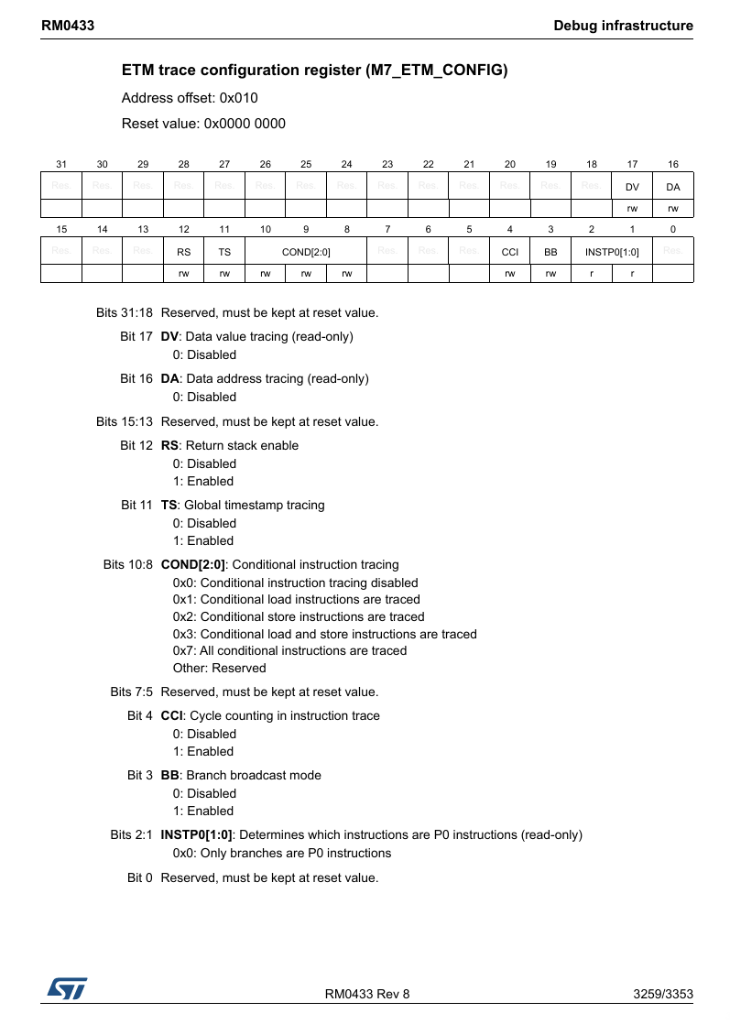
\includegraphics[width=0.88\textwidth]{figures/rm0433_etm_config_register.png}
    \caption{ساختار بیت‌های ثبّات پیکربندی ردیابی \lr{M7\_ETM\_CONFIG} برگرفته از راهنمای مرجع \lr{RM0433}}
    \label{fig:rm0433_etm_config}
\end{figure}

بررسی دقیق بیت‌های این ثبّات، مرز میان قابلیت‌های پیاده‌سازی‌شده در سیلیکون \lr{STM32H750} و مشخصات کلی استاندارد \lr{ARM} را آشکار می‌سازد:
\begin{itemize}
    \item \textbf{بیت ۱۷ (\lr{DV - Data Value Tracing}):} وضعیت فقط‌خواندنی (\lr{Read-Only}). در این پیاده‌سازی سخت‌افزاری، ردیابی مقادیر متغیرهای حافظه پشتیبانی نمی‌شود و همواره مقدار صفر دارد.
    \item \textbf{بیت ۱۶ (\lr{DA - Data Address Tracing}):} وضعیت فقط‌خواندنی (\lr{Read-Only}). ردیابی نشانی‌های داده پشتیبانی نمی‌شود و مقدار آن صفر است.
    \item \textbf{بیت ۱۲ (\lr{RS - Return Stack Enable}):} وضعیت خواندن/نوشتن (\lr{RW}). فعال کردن این بیت به ماژول \lr{ETM} اجازه می‌دهد پشته بازگشت توابع را در سخت‌افزار مدل‌سازی کند که منجر به کاهش فوق‌العاده بسته‌های انشعاب در هنگام بازگشت از زیربرنامه‌ها می‌شود.
    \item \textbf{بیت ۱۱ (\lr{TS - Global Timestamp Tracing}):} وضعیت خواندن/نوشتن (\lr{RW}). با فعال‌سازی این بیت، ماژول \lr{ETM} بسته‌های برچسب زمانی ۶۴ بیتی دریافت شده از مولد \lr{TSG} را در جریان داده‌ها منتشر می‌سازد که جهت اندازه‌گیری دقیق زمان دیوار ساعت (\lr{Wall-Clock Time}) ضروری است.
    \item \textbf{بیت‌های ۱۰ تا ۸ (\lr{COND[2:0] - Conditional Instruction Tracing}):} تعیین‌کننده نحوه پایش دستورات شرطی. مقدار \lr{\texttt{0b000}} پایش دستورات شرطی را غیرفعال کرده و مقدار \lr{\texttt{0b111}} تمامی دستورات شرطی را پایش می‌کند.
    \item \textbf{بیت ۴ (\lr{CCI - Cycle Counting in Instruction Trace}):} \textbf{حیاتی‌ترین بیت جهت سنجش \lr{WCET}}. فعال کردن این بیت سبب می‌شود ماژول \lr{ETM} دلتای تعداد چرخه‌های کلاک سپری‌شده هسته پردازنده را در جریان دستورات پایه (\lr{P0}) درج نماید. بدین ترتیب دکودر می‌تواند طول مدت اجرای هر بلوک را بر حسب چرخه‌های دقیق کلاک استخراج کند.
    \item \textbf{بیت ۳ (\lr{BB - Branch Broadcast Mode}):} در صورت فعال بودن، آدرس مقصد تمامی شاخه‌ها حتی شاخه‌های مستقیم را منتشر می‌سازد.
    \item \textbf{بیت‌های ۲ و ۱ (\lr{INSTP0[1:0]}):} وضعیت فقط‌خواندنی. مشخص‌کننده کلاس دستورات پایه (\lr{P0}) است که در این میکروکنترلر به شاخه‌ها محدود می‌باشد.
\end{itemize}

در پروژه حاضر، مقداردهی این ثبّات به صورت \lr{\texttt{ETM->CONFIG = (1U << 4) | (1U << 11);}} انجام گرفت که به طور همزمان قابلیت شمارش دقیق چرخه (\lr{CCI}) و برچسب زمانی سراسری (\lr{TS}) را برای سنجش چرخه‌ای \lr{WCET} فعال می‌سازد.

\subsection{چالش مغایرت راهنمای مرجع آی‌سی‌ها با مشخصات معماری \lr{ARM ETM}}
\label{subsec:spec_discrepancy}
یکی از مهم‌ترین یافته‌های تجربی و در عین حال اصلی‌ترین دلایل طولانی شدن فرآیند تحقیق و توسعه و پیکربندی اولیه سخت‌افزار در این پروژه، \textbf{شکاف عمیق و مغایرت ساختاری میان اسناد مرجع معماری شرکت \lr{ARM} و راهنمای مرجع سازندگان تراشه (\lr{STMicroelectronics})} بود.

در ابتدای فاز پیاده‌سازی، رویکرد متداول مهندسی ایجاب می‌کرد که از دستورالعمل رسمی شرکت \lr{ARM} در کتاب استاندارد معماری \lr{ETMv4} (\lr{ARM IHI 0064D}) استفاده شود. شکل \ref{fig:arm_spec_table} جدول معروف \lr{Table 4-15} این سند استاندارد را نشان می‌دهد که مراحل و مقادیر پیشنهادی \lr{ARM} را برای راه‌اندازی اولیه ردیابی دستورات مشخص کرده است \cite{armetmv42017}.

\begin{figure}[H]
    \centering
    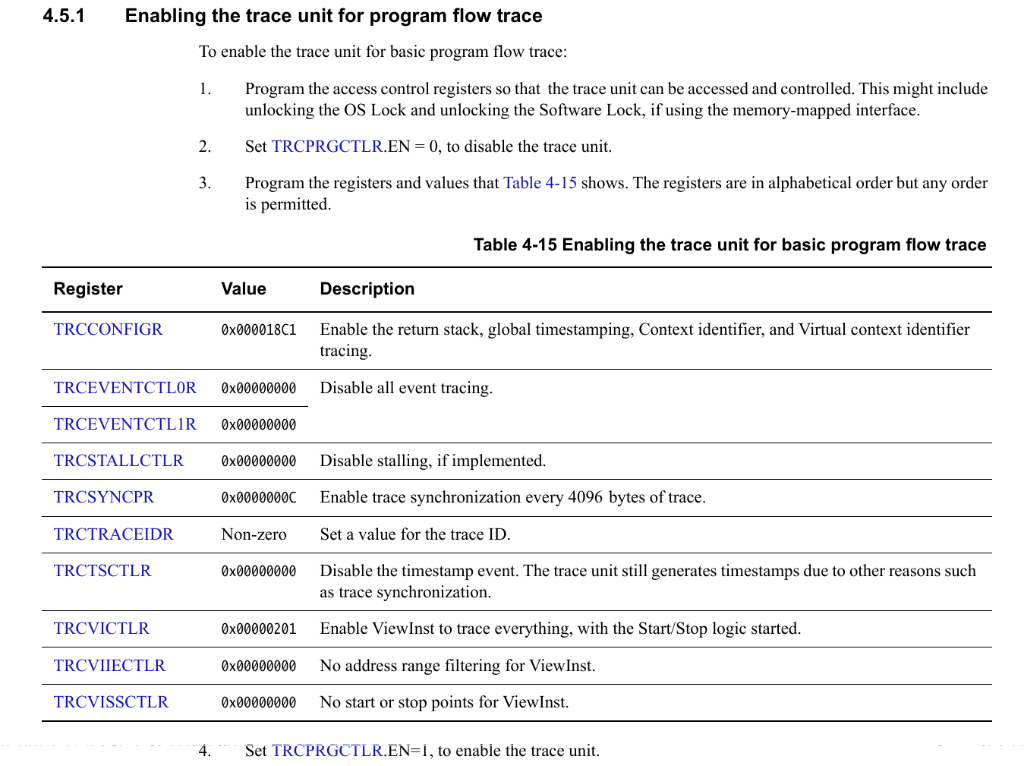
\includegraphics[width=0.88\textwidth]{figures/arm_etm_spec_enabling_table.png}
    \caption{دستورالعمل پیشنهادی فعال‌سازی ردیابی در استاندارد مرجع معماری \lr{ARM ETMv4} (جدول ۴-۱۵ سند \lr{ARM IHI 0064})}
    \label{fig:arm_spec_table}
\end{figure}

با این حال، پیاده‌سازی عینی و تلاش برای اجرای مستقیم مقادیر جدول \ref{fig:arm_spec_table} بر روی میکروکنترلر \lr{STM32H750} با شکست کامل مواجه شد. کالبدشکافی راهنمای مرجع \lr{RM0433} نشان داد که نمونه‌های ارائه‌شده در استاندارد \lr{ARM} بر روی پردازنده‌های واقعی قابل اجرای کورکورانه نیستند و هر ثبّات نیازمند تطبیق موشکافانه با جزئیات پیاده‌سازی سیلیکون است:
\begin{enumerate}
    \item \textbf{ثبّات‌های \lr{TRCVISSCTLR} و \lr{TRCVIIECTLR}:} در جدول ۴-۱۵ شرکت \lr{ARM}، صریحاً دستور داده شده که مقادیر این دو ثبّات صفر شوند تا فیلترینگ محدوده آدرس غیرفعال شود. اما در میکروکنترلر \lr{STM32H750}، ثبّات \lr{TRCVIIECTLR} اصلاً در سیلیکون پیاده‌سازی نشده و در فضای نگاشت حافظه وجود خارجی ندارد! همچنین ثبّات \lr{TRCVISSCTLR} بازطراحی شده و کنترل شروع/توقف به ثبّات‌های متفاوتی نظیر \lr{VIPCSSCTL} و \lr{VICTL} سپرده شده است. تلاش برای نوشتن در این آدرس‌ها موجب خطای دسترسی یا نادیده گرفته شدن فرمان می‌شود.
    \item \textbf{ثبّات دوره همگام‌سازی (\lr{TRCSYNCPR}):} در جدول پیشنهادی \lr{ARM}، نوشتن مقدار \lr{\texttt{0x0000000C}} (صدور همگام‌سازی هر ۴۰۹۶ بایت) توصیه شده است. اما در \lr{STM32H750}، این ثبّات از دید نرم‌افزار کاملاً \textbf{فقط‌خواندنی (\lr{Read-Only})} است و مقدار آن روی هگزادسیمال \lr{\texttt{0x0A}} ثابت نگه داشته شده است؛ بنابراین هرگونه تلاش نرم‌افزاری جهت نوشتن در این ثبّات بی‌اثر است.
    \item \textbf{مقداردهی ثبّات پیکربندی (\lr{TRCCONFIGR}):} شرکت \lr{ARM} در این جدول نوشتن مقدار \lr{\texttt{0x000018C1}} را پیشنهاد می‌دهد که بیت‌های ردیابی \lr{Context ID} و \lr{Virtual Context ID} را فعال می‌سازد. این بیت‌ها مختص پردازنده‌های رده کاربردی (\lr{Cortex-A}) با واحد مدیریت حافظه پیشرفته (\lr{MMU}) و هایپروایزر هستند. در پردازنده مایکروکنترلری \lr{Cortex-M7} این بیت‌ها یا رزرو هستند یا پیاده‌سازی نشده‌اند و نوشتن چنین مقداری وضعیت ثبّات را غیرقابل پیش‌بینی (\lr{UNPREDICTABLE}) می‌سازد.
\end{enumerate}

این مغایرت‌های بنیادین اثبات نمود که پیکربندی \lr{CoreSight} نیازمند مهندسی معکوس دقیق و اعتبارسنجی هر آفست حافظه بر اساس راهنمای مرجع اختصاصی تراشه (\lr{RM0433}) است و نمونه کدهای عمومی قابلیت اطمینان ندارند.

\section{تشریح فایل‌های راهکار نرم‌افزاری: پیاده‌سازی \lr{ETMv4.h} و \lr{ETMv4.c}}
\label{sec:firmware_implementation}
یکی از نکات حائز اهمیت در سطح معماری نرم‌افزار این است که \textbf{نه کتابخانه استاندارد هسته \lr{CMSIS} (\lr{\texttt{core\_cm7.h}}) و نه درایورهای شرکت سازنده (\lr{STM32Cube HAL})، هیچ‌گونه استراکت داده یا توابع رابطی برای ثبّات‌های \lr{ETMv4} در پردازنده \lr{Cortex-M7} فراهم نکرده‌اند!} شرکت \lr{ST} تنها ماژول‌های پایه‌ای \lr{DBGMCU} و درگاه تک‌سیمه \lr{SWO/ITM} را تعریف نموده است.

از این رو، کلیه ساختارهای داده نگاشت حافظه، ماسک‌های بیتی و توابع راه‌اندازی توسط نگارنده با مطالعه سطر به سطر اسناد \lr{RM0433 Rev 8} و \lr{ARM CoreSight v2.0} طراحی و پیاده‌سازی شد.

\subsection{ساختارهای داده در \lr{ETMv4.h}}
فایل هدر \lr{\texttt{ETMv4.h}} حاوی استراکت‌های کاملی از ماژول‌های سخت‌افزاری است:
\begin{itemize}
    \item \lr{\texttt{ETM\_TypeDef}}: ساختار کامل ثبّات‌های \lr{ETMv4} در آدرس \lr{\texttt{0xE0041000}} شامل ثبّات‌های کنترل برنامه‌ریزی (\lr{PRGCTL})، وضعیت (\lr{STAT})، پیکربندی (\lr{CONFIG})، شمارش چرخه (\lr{CCCTL})، شناسه ردیابی (\lr{TRACEID})، کنترل فیلترینگ (\lr{VICTL} و \lr{VIPCSSCTL}) و ثبّات‌های شناسایی سیلیکون (\lr{IDR0} تا \lr{IDR13}).
    \item \lr{\texttt{TPIU\_TypeDef}}: ساختار ثبّات‌های واحد اینترفیس پورت ردیابی در آدرس \lr{\texttt{0x5C015000}} شامل انتخاب اندازه پورت (\lr{CURPSIZE}) و کنترل قالب‌بندی و تخلیه (\lr{FFCR}).
    \item \lr{\texttt{CSTF\_TypeDef}}: ساختار قیف ردیابی در آدرس \lr{\texttt{0x5C013000}} جهت کنترل مالتی‌پبلکسر ورودی‌های \lr{ATB}.
    \item \lr{\texttt{ETF\_TypeDef}}: ساختار بافر \lr{FIFO} سخت‌افزاری در آدرس \lr{\texttt{0x5C014000}} جهت مدیریت جریان داده در مد \lr{Hardware FIFO}.
    \item \lr{\texttt{TSG\_TypeDef}}: ساختار مولد برچسب زمانی ۶۴ بیتی در آدرس \lr{\texttt{0x5C005000}}.
    \item \lr{\texttt{Trace\_Status\_t}}: ساختار جامع عیب‌یابی که با یک فراخوانی وضعیت تمامی ثبّات‌های مسیر ردیابی را در متغیر سراسری \lr{\texttt{g\_trace\_status}} کپی می‌کند تا در دیباگر قابل بازبینی باشد.
\end{itemize}

\subsection{توابع عملیاتی در \lr{ETMv4.c}}
پیاده‌سازی ارائه‌شده در \lr{\texttt{ETMv4.c}} شامل توابع کلیدی زیر است:
\begin{itemize}
    \item \lr{\texttt{Parallel\_Trace\_configure()}}: تابع اصلی راه‌اندازی که به ترتیب ماژول‌های پین خروجی، \lr{TPIU}، \lr{ETF}، \lr{CSTF}، \lr{TSG}، \lr{ETM} و \lr{DWT} را پیکربندی کرده و در نهایت ردیابی را فعال می‌سازد.
    \item \lr{\texttt{Disable\_ETM()}} و \lr{\texttt{Enable\_ETM()}}: وظیفه خاموش و روشن کردن ایمن هسته \lr{ETM}. تابع غیرفعال‌سازی پس از صفر کردن بیت \lr{PRGCTL.EN}، در یک حلقه منتظر ست شدن بیت‌های \lr{STAT.IDLE} و \lr{STAT.PMSTABLE} می‌ماند تا اطمینان حاصل شود خط لوله داخلی کاملاً تخلیه شده است.
    \item \lr{\texttt{DWT\_Configure()}}: مقایسه‌گرهای سخت‌افزاری شماره ۰ و ۱ ماژول \lr{DWT} را روی نشانی‌های شروع و پایان پنجره ردیابی تنظیم می‌کند.
    \item \lr{\texttt{StartPoint()}} و \lr{\texttt{StopPoint()}}: توابع نشانه‌گذار مرزهای اندازه‌گیری.
\end{itemize}

\textbf{راهکار ممانعت از بهینه‌سازی کامپایلر در توابع نشانه‌گذار:}
اگر توابع \lr{StartPoint} و \lr{StopPoint} صرفاً شامل دستورات توخالی یا مشابه‌ای مانند \lr{\texttt{nop}} باشند، بهینه‌ساز پیشرفته کامپایلر \lr{GCC} در سطوح بهینه‌سازی بالا (\lr{-Os} یا \lr{-O2}) به دلیل فعال بودن قابلیت \lr{-fipa-icf (Identical Code Folding)}، هر دو تابع را در یک نشانی یکسان در حافظه کد تجمیع می‌کند! در این صورت، نشانی تریگر شروع و پایان در \lr{DWT} برابر شده و هیچ ردیابی صورت نمی‌گیرد. برای شکستن این همسانی و ممانعت از ادغام توابع توسط کامپایلر، صفت \lr{\texttt{\_\_attribute\_\_((noinline))}} به همراه مقداردهی‌های متمایز به یک متغیر سراسری از جنس فرار (\lr{volatile}) درون توابع تزریق گردید:
\begin{latin}
\begin{lstlisting}[language=C, caption={\rl{پیاده‌سازی توابع نشانه‌گذار مرز پنجره با ممانعت از ادغام بهینه‌ساز}}]
volatile uint32_t g_gate_marker;

__attribute__((noinline)) void StartPoint(void){
    g_gate_marker = 0xA5A50001UL;
}

__attribute__((noinline)) void StopPoint(void){
    g_gate_marker = 0x5A5A0002UL;
}
\end{lstlisting}
\end{latin}

\section{روش به‌کارگیری محصول و تزریق به کدهای کاربری}
\label{sec:product_usage_workflow}
طراحی این سامانه با هدف سهولت بهره‌برداری در پروژه‌های صنعتی و دانشگاهی انجام شده است. برای استفاده از این سیستم تأمین داده ردیابی در پروژه‌های مختلف، فرآیند زیر طی می‌شود:
\begin{enumerate}
    \item افزودن فایل‌های درایور \lr{\texttt{ETMv4.h}} و \lr{\texttt{ETMv4.c}} به ساختار پروژه نرم‌افزاری میکروکنترلر.
    \item فراخوانی تابع راه‌انداز اصلی \lr{\texttt{Parallel\_Trace\_configure();}} در فاز مقداردهی اولیه سیستم (پیش از ورود به حلقه اصلی برنامه).
    \item احاطه کردن قطعه‌کد، تابع، یا حلقه مورد نظر جهت سنجش \lr{WCET} با دو فراخوانی ساده \lr{\texttt{StartPoint();}} و \lr{\texttt{StopPoint();}}.
\end{enumerate}

\subsection{تضمین عدم تداخل و حفظ رفتار غیرتهاجمی}
این روش به‌کارگیری، تضمین قطعی می‌دهد که \textbf{هیچ‌گونه تداخلی در رفتار زمانی، اولویت وقفه‌ها، یا منطق اجرایی سایر بخش‌های برنامه کاربر رخ نخواهد داد}. دلایل این قطعیت عبارتند از:
\begin{itemize}
    \item بلوک ردیابی \lr{ETM} به صورت مستقل و مستقیم با فرکانس اصلی پردازنده (\lr{CPU\_CLK}) کار می‌کند و هیچ سرباری بر خطوط لوله دستورات هسته تحمیل نمی‌نماید.
    \item تنظیمات زنجیره کلاک سیستم (\lr{PLL}ها)، مقسم‌های فرکانسی، کنترل‌کننده‌های وقفه (\lr{NVIC}) و پریفرال‌های کاربر بدون کمترین تغییر دست‌نخورده باقی می‌مانند.
    \item تنها تغییرات سخت‌افزاری اعمال‌شده، فعال‌سازی ماژول‌های زیرساخت دیباگ (\lr{CoreSight}) و تغییر پیکربندی پایه‌های اختصاصی ردیابی (\lr{PE2} تا \lr{PE6}) است که در کاربردهای عادی آزاد هستند.
\end{itemize}

\subsection{محدودیت نرخ‌های نمونه‌برداری سخت‌افزاری لاجیک آنالایزر}
نکته بسیار مهم در استفاده عملیاتی از این فرم‌ور، هماهنگی فرکانسی با ابزار گیرنده خارجی است. لاجیک آنالایزرهای دیجیتال (نظیر \lr{DSLogic U3Pro16}) از فرکانس‌های نمونه‌برداری گسسته و از پیش‌تعیین‌شده‌ای پشتیبانی می‌کنند. شکل \ref{fig:dslogic_sample_rates} منوی فرکانس‌های مجاز نمونه‌برداری در نرم‌افزار لاجیک آنالایزر مورد استفاده را نمایش می‌دهد.

\begin{figure}[H]
    \centering
    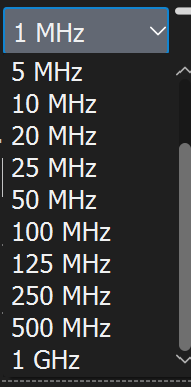
\includegraphics[width=0.35\textwidth]{figures/dslogic_sample_rates_menu.png}
    \caption{فرکانس‌های مجاز و گسسته نمونه‌برداری در نرم‌افزار لاجیک آنالایزر \lr{DSLogic}}
    \label{fig:dslogic_sample_rates}
\end{figure}

مطابق با شکل \ref{fig:dslogic_sample_rates}، نرخ‌های نمونه‌برداری دستگاه منحصراً به مقادیر ۱، ۵، ۱۰، ۲۰، ۲۵، ۵۰، ۱۰۰، ۱۲۵، ۲۵۰، ۵۰۰ مگاهرتز و ۱ گیگاهرتز محدود است. 

همان‌طور که در فصل چهارم اثبات شد، برای نمونه‌برداری پایدار و بدون خطای جیتر از لبه‌های کلاک پورت موازی، حداقل نسبت بیش‌نمونه‌برداری ۱۰ برابری ($10\times$) مورد نیاز است. کلاک پورت ردیابی (\lr{TRACECLK}) معمولاً نصف کلاک هسته پردازنده است ($f_{\mathrm{trace}} = f_{\mathrm{CPU}} / 2$). بنابراین:
\begin{itemize}
    \item اگر پردازنده در فرکانس ۲۰ مگاهرتز تنظیم شود، کلاک \lr{Trace} ۱۰ مگاهرتز بوده و با نرخ نمونه‌برداری ۱۰۰ مگاهرتز (۱۰ برابر) یا ۲۵۰ مگاهرتز (۲۵ برابر) لاجیک آنالایزر به طور کامل همخوانی دارد.
    \item اما اگر پردازنده در یک فرکانس کاری اختیاری غیرمنطبق (مثلاً ۴۸۰ مگاهرتز) تنظیم گردد، کلاک \lr{Trace} ۲۴۰ مگاهرتز خواهد شد که به نرخ نمونه‌برداری ۲.۴ گیگاهرتز نیاز دارد؛ نرخی که فراتر از سقف ۱ گیگاهرتزی لاجیک آنالایزر بوده و در منوی سخت‌افزار وجود ندارد.
\end{itemize}
بنابراین، در حال حاضر کاربر برای نمونه‌برداری معتبر سیگنال‌های \lr{Trace}، باید فرکانس کاری پردازنده را متناسب با نرخ‌های گسسته موجود در ابزار نمونه‌برداری انتخاب نماید.

\section[چالش بسته‌های همگام‌سازی (\lr{A-Sync}) و آسیب‌شناسی روش سوئیچینگ]{چالش بسته‌های همگام‌سازی (\lr{A-Sync})\\ و آسیب‌شناسی روش سوئیچینگ}
\label{sec:async_deep_dive}

\subsection[کشف ریشه خطای \lr{NO\_SYNC} و تصحیح وضعیت ثبّات \lr{TRCSYNCPR}]{کشف ریشه خطای \lr{NO\_SYNC}\\ و تصحیح وضعیت ثبّات \lr{TRCSYNCPR}}
\label{subsec:no_sync_issue}
در فازهای نخست پایش قطعه‌کدهای بسیار کوتاه (نظیر اجرای یک حلقه یا روتین وقفه با طول زمانی کمتر از ۵۰ میکروثانیه)، خطای عدم تطبیق در موتور دکودر \lr{OpenCSD} پدیدار می‌شد:
\begin{latin}
\begin{lstlisting}[language=bash]
OpenCSD: Trace un-synced - waiting for sync packet (NO_SYNC)
Error: Frame synchronization failed. 0 instructions reconstructed.
\end{lstlisting}
\end{latin}

کالبدشکافی جریان بایت‌ها ریشه این خطا را روشن ساخت:
\begin{itemize}
    \item دکودر نرم‌افزاری جهت تطبیق دادن بایت‌های فشرده اتم (\lr{E/N}) با باینری \lr{ELF}، لزوماً نیازمند دانستن «آدرس مبدأ مطلق» است که توسط بسته همگام‌سازی دستورالعمل (\lr{I\_SYNC / A-Sync}) حمل می‌شود.
    \item در معماری \lr{ETMv4}، ارسال بسته‌های \lr{I\_SYNC} بر عهده شمارنده داخلی است که دوره‌ای بودن آن به ثبّات \lr{TRCSYNCPR} منتهی می‌شود.
    \item \textbf{نکته حیاتی و تصحیح در گزارش:} در میکروکنترلر \lr{STM32H750}، ثبّات \lr{TRCSYNCPR} در سیلیکون به صورت کاملاً \textbf{فقط‌خواندنی (\lr{Read-Only})} پیاده‌سازی شده و مقدار آن به طور سخت‌افزاری بر روی مقدار هگزادسیمال \lr{\texttt{0x0A}} قفل است (معادل $2^{10} = 1024$ بایت). در نسخه‌های ابتدایی درایور، کدهایی جهت نوشتن مقادیر کوچکتری نظیر \lr{\texttt{0x08}} در این ثبّات وجود داشت؛ اما به دلیل ماهیت فقط‌خواندنی بودن، این عملیات توسط سخت‌افزار نادیده گرفته می‌شد.
    \item در قطعه‌کدهای کوتاه‌مدت، حجم کل داده‌های ردیابی تولیدشده تنها در حدود \textbf{۲۸ تا ۴۸ بایت} بود. از آنجا که حجم داده به سقف سخت‌افزاری ۱۰۲۴ بایت نمی‌رسید، سخت‌افزار هیچ بسته همگام‌سازی صادر نمی‌کرد و دکودر به دلیل فقدان نشانی اولیه قادر به رمزگشایی جریان نبود.
\end{itemize}

\subsection{روش ابداعی سوئیچینگ \lr{TRCPRGCTLR.EN} و آسیب‌شناسی آن}
\label{subsec:switching_drawbacks}
برای حل معضل بسته‌های همگام‌سازی، با اتکا به یک ویژگی معماری کشف‌شده در استاندارد \lr{ARM} مبنی بر این که:
\begin{quote}
\textit{«تغییر وضعیت بیت برنامه‌ریزی \lr{TRCPRGCTLR.EN} از صفر به یک، ماشین حالت \lr{ETM} را ریست کرده و سخت‌افزار را قانوناً ملزم می‌سازد تا در نخستین فریم خروجی، یک بسته همگام‌سازی اجباری اولیه (\lr{Initial I\_SYNC}) منتشر نماید.»}
\end{quote}
ایده خاموش و روشن کردن پویا و مقطعی ماژول \lr{ETM} در شروع هر پنجره آزمون پیاده‌سازی گردید. با این حال، ارزیابی‌های دقیق‌تر پرده از نقایص و خطرات این روش برداشت.

\textbf{مشکلات و آسیب‌شناسی روش خاموش و روشن کردن مکرر \lr{ETM}:}
\begin{enumerate}
    \item \textbf{از بین رفتن پیوستگی و یکپارچگی جریان ردیابی:} خاموش و روشن کردن پی‌درپی \lr{ETM} موجب شکستن پیوستگی زمانی داده‌ها می‌شود. در هر بار خاموش شدن، پایپ‌لاین فشرده‌سازی بازنشانی شده و تاریخچه ثبت شاخه‌ها پاک می‌گردد. در نتیجه، لاگ خروجی حاوی قطعات ناپیوسته و نامفهوم خواهد بود.
    \item \textbf{عدم تخلیه کامل بافر ردیابی (\lr{Buffer Drain Truncation}):} هنگامی که \lr{ETM} به صورت ناگهانی غیرفعال (\lr{Disable}) می‌شود، داده‌های ردیابی مربوط به آخرین دستورالعمل‌های اجراشده هنوز در بافرهای \lr{FIFO} داخلی ماژول و رم \lr{ETF} قرار دارند و فرصت انتقال کامل به پورت \lr{TPIU} را پیدا نکرده‌اند. در نتیجه، بخش انتهایی قطعه‌کد مورد سنجش دور ریخته شده یا با خطا مواجه می‌گردد.
\end{enumerate}

\textbf{راهکار مطمئن (\lr{Robust}) نهایی: \lr{Trace} ممتد در یک پنجره‌ و فیلترینگ نرم‌افزاری در دکودر:}
برای عبور بنیادین از این مشکلات، بهترین و قابل‌اعتمادترین رویکرد مهندسی آن است که:
\begin{itemize}
    \item ماژول \lr{ETM} در طول اجرای برنامه در یک پنجره زمانی متوالی، پیوسته روشن و فعال بماند تا هیچ بسته‌ای به دلیل قطع و وصل ناگهانی مفقود نگردد و یکپارچگی خط لوله فشرده‌سازی حفظ شود.
    \item در سمت کامپیوتر میزبان، اسکریپت دکودر پس از رمزگشایی کامل جریان بایت‌ها، در لاگ خروجی به جستجوی رخدادهای ورود به تابع \lr{StartPoint} و خروج از \lr{StopPoint} بپردازد.
\end{itemize}
گرچه این رویکرد به دلیل ثبت پیوسته دستورات حجم بایت‌های بیشتری تولید کرده و بار پردازشی دکودر را افزایش می‌دهد، اما داده‌هایی کاملاً یکپارچه، بدون مفقودی و فوق‌العاده مطمئن (\lr{Robust}) برای سنجش قطعی \lr{WCET} فراهم می‌سازد.

\section{جمع‌بندی فصل}
در این فصل پروتکل فشرده‌سازی داده‌ها در \lr{ETMv4}، معماری زیرساخت دیباگ در میکروکنترلر \lr{STM32H750} و دامنه‌های توان و کلاک آن تبیین شد. تشریح جامع ثبّات پیکربندی \lr{TRCCONFIGR}، ارائه شواهد مغایرت اسناد \lr{ARM} با راهنمای مرجع تراشه‌ها، معرفی فایل‌های درایور اختصاصی \lr{\texttt{ETMv4.h}} و \lr{\texttt{ETMv4.c}}، بررسی روش‌های به‌کارگیری و تزریق خودکار کد، و در نهایت ریشه‌یابی چالش بسته‌های \lr{A-Sync} و آسیب‌شناسی روش‌های سوئیچینگ \lr{ETM} مستند گردید. با تسلط بر این زیرساخت سخت‌افزاری و سیستم نرم‌افزاری روی تراشه، زمینه برای بررسی نحوه دریافت و رمزگشایی بایت‌ها در فصل ششم فراهم گردیده است.


% فصل ششم: پردازش و رمزگشایی Trace
% ==============================================================================
% فصل ششم: پردازش و رمزگشایی Trace
% ==============================================================================

\chapter{پردازش و رمزگشایی \lr{Trace}}
\label{ch:decoding}

\section{مقدمه}
داده‌های دیجیتال خام ثبت‌شده بر روی حافظه لاجیک‌آنالایزر، دنباله‌ای از نمونه‌های ولتاژ ناهمگام هستند که بدون طی یک خط‌لوله پردازش نرم‌افزاری، فاقد معنای محاسباتی می‌باشند. پروتکل فشرده‌سازی \lr{ETMv4} یک جریان کاملاً غیرخطی از تصمیمات انشعاب و رویدادهای سیستمی است که باید با کدهای باینری فایل کامپایل‌شده (\lr{ELF}) تلفیق شود تا به دستورات متوالی زبان اسمبلی و زمان‌بندی دقیق تبدیل گردد. برای تحقق این هدف، اسکریپت پیشرفته پایتون موسوم به \lr{\texttt{TraceStreamProcessor.py}} طراحی و پیاده‌سازی شد. این ابزار به عنوان موتور اصلی پیش‌پردازش، وظیفه استخراج بایت‌های فریم پورت \lr{TPIU}، اعتبارسنجی یکپارچگی سیگنال‌ها، ساختاربندی اسنپ‌شات استاندارد و ادغام با موتور مرجع صنعتی \lr{OpenCSD} را بر عهده دارد. در این فصل، کالبدشکافی خط‌لوله پردازش داده، ساختار فایل‌های اسنپ‌شات، پیوند عمیق پارامترهای دکودر با ثبّات‌های سخت‌افزاری پردازنده، و در نهایت طراحی و پیاده‌سازی افزونه اختصاصی محیط توسعه \lr{VS Code} موسوم به \lr{CoreSight Trace Studio} جهت اتوماسیون کامل این فرآیندها تشریح می‌گردد.

\section[معماری اسکریپت پردازش داده \lr{TraceStreamProcessor.py}]{معماری اسکریپت پردازش داده\\ (\lr{TraceStreamProcessor.py})}
\label{sec:tracestreamprocessor_arch}
اسکریپت \lr{\texttt{TraceStreamProcessor.py}} به عنوان پل ارتباطی هوشمند میان لایه سخت‌افزار ثبت سیگنال و موتور نرم‌افزاری رمزگشای مرجع \lr{OpenCSD} عمل می‌کند. در رویکردهای اولیه، رمزگشایی مستقیم داده‌های خام با خطاهای متعددی نظیر عدم تراز فاز، گم‌شدن مرز فریم‌ها و ناسازگاری قالب مواجه می‌شد. برای غلبه بر این مسائل، خط‌لوله‌ای هفت‌مرحله‌ای و کاملاً خودکار پیاده‌سازی گردید که وظایف تبدیل، ترازسازی، اعتبارسنجی و بسته‌بندی را انجام می‌دهد. شکل \ref{fig:tracestreamprocessor_flow} فلوچارت مراحل اجرایی این اسکریپت را به تصویر کشیده است.

\begin{figure}[H]
\centering
\begin{latin}
\begin{tikzpicture}[
    node distance=0.42cm,
    stepb/.style={rectangle, draw=blue!80, fill=blue!5, thick, rounded corners=4pt, text width=13.2cm, align=center, inner sep=4pt},
    arr/.style={-latex, very thick, draw=black!70}
]
    \node [stepb] (s1) {\textbf{\rl{گام ۱: فراخوانی فایل نمونه‌های خام لاجیک‌آنالایزر}}\\[0.05cm]\small \rl{خواندن فایل} \lr{CSV} \rl{شامل نمونه‌های زمانی} \lr{TRACECLK} \rl{و ۴ خط داده} \lr{TRACED0..3}};
    
    \node [stepb, below=0.42cm of s1] (s2) {\textbf{\rl{گام ۲: آشکارسازی لبه‌های کلاک و فیلترینگ جهش‌ها (\lr{Glitch Filtering})}}\\[0.05cm]\small \rl{تشخیص لبه‌های معتبر کلاک، استخراج نیبل‌های ۴ بیتی و حذف نویز با پایدارسازی نمونه‌ها}};
    
    \node [stepb, below=0.42cm of s2] (s3) {\textbf{\rl{گام ۳: ترکیب نیبل‌ها و بازسازی بایت‌های فریم \lr{TPIU}}}\\[0.05cm]\small \rl{جفت‌سازی نیبل کم‌ارزش و پرارزش جهت تشکیل بایت‌های متوالی پروتکل سیم}};
    
    \node [stepb, below=0.42cm of s3] (s4) {\textbf{\rl{گام ۴: اعتبارسنجی فریم‌ها، ترازسازی بر پایه \lr{FSYNC} و حذف قطعات ناقص}}\\[0.05cm]\small \rl{بررسی دوره‌ای الگوهای} \lr{FSYNC/HSYNC}\rl{، رتبه‌بندی تراز فاز با بسته‌های} \lr{A-Sync}\rl{، و ترازسازی ۱۶ بایتی}};
    
    \node [stepb, below=0.42cm of s4] (s5) {\textbf{\rl{گام ۵: تفکیک سگمنت‌های بارگذاری (\lr{PT\_LOAD}) از باینری \lr{ELF}}}\\[0.05cm]\small \rl{پارس ساختار باینری ۳۲ بیتی، استخراج محتوای حافظه فلش و تولید فایل‌های دامپ} \texttt{mem\_*.bin}};
    
    \node [stepb, below=0.42cm of s5] (s6) {\textbf{\rl{گام ۶: ساختاربندی خودکار بسته اسنپ‌شات استاندارد \lr{OpenCSD}}}\\[0.05cm]\small \rl{تولید فایل‌های پیکربندی} \texttt{snapshot.ini}\rl{،} \texttt{device1.ini}\rl{،} \texttt{device2.ini} \rl{و} \texttt{trace.ini}};
    
    \node [stepb, below=0.42cm of s6] (s7) {\textbf{\rl{گام ۷: فراخوانی موتور رمزگشای \lr{trc\_pkt\_lister} و استخراج لاگ دستورات}}\\[0.05cm]\small \rl{رمزگشایی چرخه‌دقیق دستورالعمل‌ها، تفکیک روتین‌های وقفه، و محاسبه زمان اجرای بدترین شرایط (\lr{WCET})}};

    \draw [arr] (s1) -- (s2);
    \draw [arr] (s2) -- (s3);
    \draw [arr] (s3) -- (s4);
    \draw [arr] (s4) -- (s5);
    \draw [arr] (s5) -- (s6);
    \draw [arr] (s6) -- (s7);
\end{tikzpicture}
\end{latin}
\caption{فلوچارت خط‌لوله پردازش هفت‌مرحله‌ای اسکریپت \lr{\texttt{TraceStreamProcessor.py}}}
\label{fig:tracestreamprocessor_flow}
\end{figure}

\section[کالبدشکافی فنی مراحل پردازش در \lr{TraceStreamProcessor}]{کالبدشکافی فنی مراحل پردازش در\\ \lr{TraceStreamProcessor}}
\label{sec:processing_stages_deepdive}

\subsection{آشکارسازی لبه، حذف گلیچ و استخراج نیبل‌ها}
در مد ردیابی موازی ۴ بیتی، هر بایت داده شامل دو نیبل ۴ بیتی است که در لبه‌های کلاک پورت \lr{TPIU} صادر می‌شوند. سیگنال‌های دریافتی از لاجیک‌آنالایزر با نرخ اورسمپلینگ ۱۰ برابری ثبت شده‌اند؛ بنابراین هر دوره تناوب کلاک با چندین نمونه دیجیتال نشان داده می‌شود. اسکریپت برای ممانعت از خطاهای ناشی از نویزهای ضربه‌ای و جهش‌های ولتاژی (\lr{Glitches})، از یک مکانیزم فیلترینگ پایداری لبه استفاده می‌کند: یک نیبل تنها زمانی معتبر شناخته می‌شود که وضعیت کلاک نسبت به نمونه پیشین تغییر کرده و برای حداقل یک نمونه در وضعیت جدید پایدار بماند. قطعه‌کد \ref{lst:nibble_extraction} پیاده‌سازی این منطق را نشان می‌دهد:

\begin{latin}
\begin{lstlisting}[language=Python, caption={\rl{منطق آشکارسازی لبه کلاک و استخراج نیبل‌ها در} \lr{\texttt{TraceStreamProcessor.py}}}, label={lst:nibble_extraction}]
def nibbles_from_csv(path):
    """
    Recover TRACEDATA nibbles from DSLogic oversampled CSV export.
    Rejects single-sample glitches by ensuring the clock state
    persists after an edge transition.
    """
    CLK_COL, D0_COL, D1_COL, D2_COL, D3_COL = 1, 2, 3, 4, 5
    nibbles = bytearray()
    prev_raw_clk = None

    with open(path, "r") as f_in:
        for row in csv.reader(f_in):
            if not row or row[0].startswith(";") or "Time" in row[0]:
                continue
            try:
                raw_clk = int(row[CLK_COL])
                nib = ((int(row[D3_COL]) << 3) | (int(row[D2_COL]) << 2) |
                       (int(row[D1_COL]) << 1) | int(row[D0_COL]))
            except (ValueError, IndexError):
                continue

            if prev_raw_clk is None:
                prev_raw_clk = raw_clk
                continue

            # Clock edge detected
            if raw_clk != prev_raw_clk:
                nibbles.append(nib)
                prev_raw_clk = raw_clk

    return nibbles
\end{lstlisting}
\end{latin}

\subsection{ترازسازی فریم‌های پروتکل \lr{TPIU} بر پایه الگوهای \lr{FSYNC}}
در استاندارد معماری \lr{CoreSight}، بایت‌های ردیابی مستقیماً به صورت خام بر روی سیم منتشر نمی‌شوند؛ بلکه در قالب فریم‌های ۱۶ بایتی پروتکل واسط پورت \lr{TPIU} بسته‌بندی می‌گردند. در این فریم‌ها:
\begin{itemize}
    \item بایت پانزدهم (بایت آخر) به عنوان بایت کمکی (\lr{Auxiliary Byte}) عمل می‌کند که بیت‌های کم‌ارزش بایت‌های زوج و نشانگرهای تغییر شناسه جریان (\lr{ATB ID}) را در خود جای داده است.
    \item برای همگام‌سازی فریم‌ها، الگوهای ویژه \lr{FSYNC} با توالی هگزادسیمال \lr{\texttt{0x7FFFFFFF}} (۴ بایت: \texttt{FF FF FF 7F}) به طور منظم در جریان داده ارسال می‌شوند. همچنین در زمان‌های بیکاری پورت، بایت‌های پرکننده \lr{HSYNC} با مقدار \lr{\texttt{0x7FFF}} (۲ بایت: \texttt{FF 7F}) درج می‌گردند.
\end{itemize}

یکی از دستاوردهای برجسته اسکریپت \lr{\texttt{TraceStreamProcessor.py}}، کشف این حقیقت مهندسی بود که \textbf{بایت‌های سیم نباید پیش از ارسال به \lr{OpenCSD} به‌صورت دستی دی‌فریم (\lr{De-frame}) شوند!} در نسخه‌های ابتدایی، اسکریپت سعی در حذف دستی بایت‌های همگام‌سازی و جداسازی بایت‌های داده داشت که به دلیل لغزش فاز موجب خطای غیرقابل‌رفع \lr{I\_BAD\_SEQUENCE} در موتور دکودر می‌شد. در نسخه توسعه‌یافته حاضر، بایت‌های کامل سیم همراه با الگوهای همگام‌سازی در قالب فایل باینری \lr{\texttt{tpiu\_wire.bin}} حفظ شده و با تعریف فرمت \lr{\texttt{coresight}} در فایل پیکربندی، دی‌فریم کردن و تطبیق فاز به دی‌فرمتور داخلی و بهینه‌شده موتور \lr{OpenCSD} واگذار می‌گردد. اسکریپت با اسکن الگوهای \lr{FSYNC}، ابتدای بافر را به نخستین فریم معتبر ۱۶ بایتی تراز کرده و قطعات ناقص ضبط اولیه و انتهایی را پیراست (\lr{Trim}) می‌نماید.

\subsection{تفکیک خودکار سگمنت‌های اجرایی باینری (\lr{ELF Reader})}
موتور رمزگشای \lr{OpenCSD} برای اینکه بتواند بسته‌های ردگیری (شامل تصمیمات انشعاب شرطی) را به کدهای اسمبلی تبدیل کند، نیازمند دسترسی به تصویر کدهای باینری موجود در حافظه فلش میکروکنترلر است. اسکریپت \lr{\texttt{TraceStreamProcessor.py}} دارای یک ماژول مستقل پارسر فایل‌های باینری \lr{ELF} ۳۲ بیتی با فرمت لیتل‌اندیان (\lr{Little-Endian}) است که بدون وابستگی به تولچین‌های سنگین خارجی (نظیر \lr{arm-none-eabi-objcopy})، مستقیماً هدرهای برنامه (\lr{Program Headers}) را کاوش نموده و سگمنت‌های با فلگ \lr{\texttt{PT\_LOAD}} را که حاوی کدهای اجرایی برنامه کاربر هستند استخراج می‌کند. محتوای این سگمنت‌ها به عنوان فایل‌های دامپ حافظه (نظیر \lr{\texttt{mem\_08000000.bin}}) در پوشه اسنپ‌شات ذخیره می‌شوند.

\section{ادغام با موتور رمزگشای مرجع \lr{OpenCSD}}
\label{sec:opencsd_integration}
پس از ایجاد و ساختاربندی پوشه اسنپ‌شات، اسکریپت ابزار خط فرمان استاندارد \lr{trc\_pkt\_lister} متعلق به بنیاد \lr{Linaro} را با دستور زیر فراخوانی می‌کند:

\begin{latin}
\begin{lstlisting}[language=bash]
trc_pkt_lister -ss_dir ./snapshot/ -tpiu_hsync -decode -logstdout \
               -o decoded_trace.txt
\end{lstlisting}
\end{latin}

در این دستور، فلگ \lr{\texttt{-tpiu\_hsync}} دی‌فرمتور سخت‌افزاری \lr{OpenCSD} را فعال می‌سازد تا بسته‌های پرکننده همگام‌سازی را حذف نماید و آرگومان \lr{\texttt{-decode}} دستور می‌دهد که کدهای باینری با جریان ردگیری تلفیق شده و دستور به دستور بازسازی گردند. عملیات دکود در سه لایه پردازشی انجام می‌گیرد:
\begin{enumerate}
    \item \textbf{پردازشگر بسته‌ها (\lr{Packet Processor}):} بایت‌های ورودی را به عناصر سازنده پروتکل \lr{ETMv4} شامل بسته‌های همگام‌سازی (\lr{I\_SYNC})، بسته‌های اتم (\lr{ATOM})، برچسب زمانی (\lr{TIMESTAMP})، شمارش چرخه (\lr{CYCLE\_COUNT}) و استثناها (\lr{EXCEPTION}) تجزیه می‌کند.
    \item \textbf{رمزگشای دستورات (\lr{Instruction Decoder}):} با استخراج نشانی شروع برنامه از بسته \lr{I\_SYNC}، کدهای ماشین را در سگمنت‌های بارگذاری‌شده دنبال می‌کند. با برخورد به دستورات انشعاب شرطی، وضعیت شاخه را از بیت‌های بسته اتم خوانده و مسیر واقعی اجرای برنامه را بازسازی می‌نماید.
    \item \textbf{قالب‌بندی عناصر ردگیری (\lr{Trace Element Formatter}):} جریان زمانی دستورات را همراه با نشانی دستور، کد اسمبلی، نام تابع مبدأ، شماره خط در کد مبدأ و شماره چرخه ماشین در قالب فایل متنی ساختاریافته استخراج می‌کند.
\end{enumerate}

\section{کالبدشکافی ساختار فایل‌های اسنپ‌شات \lr{OpenCSD}}
\label{sec:snapshot_structure}

\subsection{ساختار و محتوای فایل‌های پوشه اسنپ‌شات}
پوشه اسنپ‌شات تولیدشده توسط \lr{\texttt{TraceStreamProcessor.py}} یک کپسول کاملاً مستقل و خودکفا از شرایط تست، اتصالات سخت‌افزاری و جریان داده‌هاست. این پوشه شامل پنج جزء کلیدی است:

\paragraph*{۱. فایل پیکربندی ریشه (\lr{\texttt{snapshot.ini}}):}
این فایل به عنوان مانیفست اصلی دکودر عمل کرده و مشخصات نسخه پروتکل، اسامی فایل‌های توصیف تجهیزات و فایل متادیتای بافر را تعیین می‌کند:
\begin{latin}
\begin{lstlisting}[language=make, caption={\rl{محتوای فایل مانیفست ریشه} \lr{\texttt{snapshot.ini}}}]
[snapshot]
version=1.0

[device_list]
device1=device1.ini
device2=device2.ini

[trace]
metadata=trace.ini
\end{lstlisting}
\end{latin}

\paragraph*{۲. فایل توصیف هسته پردازنده (\lr{\texttt{device1.ini}}):}
این فایل معماری هسته پردازنده، وضعیت اولیه ثبّات‌های کنترلی آن، و ارجاع به قطعات استخراج‌شده از حافظه فلش فایل \lr{ELF} برنامه را تعریف می‌نماید:
\begin{latin}
\begin{lstlisting}[language=make, caption={\rl{محتوای فایل توصیف هسته} \lr{\texttt{device1.ini}}}]
[device]
name=Cortex-M7_0
class=core
type=Cortex-M7

[regs]
PC=0x08000000
xPSR=0x01000000

[dump1]
file=mem_08000000.bin
address=0x08000000
length=0x1E4A0
\end{lstlisting}
\end{latin}

\paragraph*{۳. فایل توصیف منبع ردگیری و ثبّات‌های سخت‌افزاری (\lr{\texttt{device2.ini}}):}
این فایل هویت منبع ردگیری را با نام \lr{\texttt{CSETM\_0}} و کلاس \lr{\texttt{trace\_source}} تعیین کرده و حیاتی‌ترین اطلاعات مورد نیاز دکودر یعنی \textbf{مقادیر ثبّات‌های سخت‌افزاری ماژول \lr{ETM}} را در خود جای داده است:
\begin{latin}
\begin{lstlisting}[language=make, caption={\rl{محتوای فایل منبع ردگیری و ثبّات‌های سخت‌افزاری} \lr{\texttt{device2.ini}}}]
[device]
name=CSETM_0
class=trace_source
type=ETM4.0

[regs]
TRCCONFIGR(0x4)=0x00000811
TRCEVENTCTL0R(0x8)=0x00000000
TRCEVENTCTL1R(0x9)=0x00000000
TRCSTALLCTLR(0xB)=0x00000000
TRCTSCTLR(0xC)=0x00000000
TRCSYNCPR(0xD)=0x0000000A
TRCCCCTLR(0xE)=0x00000040
TRCTRACEIDR(0x10)=0x0000003E
TRCVICTLR(0x20)=0x00000201
TRCVIIECTLR(0x21)=0x00000000
TRCVISSCTLR(0x22)=0x00000000
TRCVIPCSSCTLR(0x23)=0x00020001
TRCIDR8(0x60)=0x00000001
TRCIDR9(0x61)=0x00000000
TRCIDR10(0x62)=0x00000000
TRCIDR11(0x63)=0x00000000
TRCIDR12(0x64)=0x00000001
TRCIDR13(0x65)=0x00000000
TRCIDR0(0x78)=0x080006E1
TRCIDR1(0x79)=0x4100F401
TRCIDR2(0x7A)=0x00000004
TRCIDR3(0x7B)=0x07090004
TRCIDR4(0x7C)=0x00114000
TRCIDR5(0x7D)=0x90C70002
TRCAUTHSTATUS(0x3EE)=0x000000C0
\end{lstlisting}
\end{latin}

\paragraph*{۴. فایل متادیتای بافر و توپولوژی ارتباطات (\lr{\texttt{trace.ini}}):}
این فایل ساختار ارتباطی گذرگاه‌ها و نحوه هدایت داده‌ها از پورت فیزیکی به موتور نرم‌افزاری را تبیین می‌سازد:
\begin{latin}
\begin{lstlisting}[language=make, caption={\rl{محتوای فایل توپولوژی بافر} \lr{\texttt{trace.ini}}}]
[trace_buffers]
buffers=buffer0

[buffer0]
name=TPIU_WIRE
file=tpiu_wire.bin
format=coresight

[core_trace_sources]
Cortex-M7_0=CSETM_0

[source_buffers]
CSETM_0=TPIU_WIRE
\end{lstlisting}
\end{latin}

\subsection{انطباق پارامترهای اسنپ‌شات با ثبّات‌های فیزیکی پردازنده}
یک نکته بنیادین که در این پژوهش اثبات گردید آن است که: \textbf{موتور رمزگشای \lr{OpenCSD} بدون آگاهی دقیق از مقادیر ثبّات‌های سخت‌افزاری پردازنده بر روی سیلیکون، به هیچ عنوان قادر به رمزگشایی صحیح داده‌ها نخواهد بود.} بخش \lr{\texttt{[regs]}} در فایل \lr{\texttt{device2.ini}} دقیقاً حامل مقادیر همان ثبّات‌هایی است که در فصل پنجم در فریمورک میکروکنترلر و در تابع \lr{\texttt{ETM\_Configure()}} مقداردهی شده‌اند:
\begin{itemize}
    \item \textbf{ثبّات \lr{TRCCONFIGR} (آفست \lr{\texttt{0x010}}، شناسه \lr{\texttt{0x4}}):} این ثبّات تعیین می‌کند که چه امکاناتی فعال بوده‌اند. در پروژه حاضر، مقدار هگزادسیمال \lr{\texttt{0x00000811}} نشان‌دهنده فعال بودن شمارش دقیق چرخه‌ها (\lr{CCI} - بیت ۴)، برچسب زمانی سراسری (\lr{TS} - بیت ۱۱) و فعال بودن موتور ردیابی است. اگر دکودر از فعال بودن این بیت‌ها مطلع نباشد، بایت‌های مربوط به شمارنده‌ها را به عنوان بایت‌های نامعتبر تلقی کرده و خروجی با خطای مهلک مواجه می‌شود.
    \item \textbf{ثبّات \lr{TRCCCCTLR} (آفست \lr{\texttt{0x038}}، شناسه \lr{\texttt{0xE}}):} آستانه صدور بسته‌های چرخه‌ای را تعیین می‌کند (مقدار \lr{\texttt{0x40}} معادل ۶۴ چرخه). دکودر با دانستن این مقدار، فواصل زمانی میان دستورات متوالی را تخمین می‌زند.
    \item \textbf{ثبّات \lr{TRCSYNCPR} (آفست \lr{\texttt{0x034}}):} مشخص‌کننده دوره صدور بسته‌های همگام‌سازی اجباری (\lr{I\_SYNC}) است که در سیلیکون \lr{STM32H750} روی مقدار ثابت \lr{\texttt{0x0A}} ($2^{10} = 1024$ بایت) قفل است.
    \item \textbf{ثبّات \lr{TRCTRACEIDR} (آفست \lr{\texttt{0x040}}):} شناسه منبع در گذرگاه \lr{ATB} (مقدار \lr{\texttt{0x3E}}) است. دکودر در لایه فریم‌زدایی \lr{TPIU}، بسته‌های مربوط به این شناسه را فیلتر کرده و به موتور \lr{ETMv4} تحویل می‌دهد.
    \item \textbf{ثبّات‌های فیلترینگ (\lr{TRCVIPCSSCTLR} و \lr{TRCVICTLR}):} تعیین‌کننده تریگرهای شروع و پایان پنجره ردگیری توسط مقایسه‌گرهای \lr{DWT} هستند که وضعیت پنجره پایش فعال را به دکودر اعلام می‌نمایند.
\end{itemize}

\section{مدیریت مرزهای وقفه و کانتکست‌های پردازنده}
\label{sec:isr_and_context_management}
یکی از توانمندی‌های برجسته این خط‌لوله، تشخیص تمیز ورود و خروج به روتین‌های وقفه (\lr{ISR}) است. در پردازنده \lr{Cortex-M7}، وقوع وقفه موجب درج خودکار فریم پشته بر روی \lr{MSP} و صدور مقدار بازگشت ویژه \lr{EXC\_RETURN} (نظیر \texttt{0xFFFFFFF9}) می‌گردد. خط‌لوله پایتون با تحلیل عناصر رویداد استثنا (\lr{Exception Packets}) در موتور \lr{OpenCSD} و بازگشت با دستور \texttt{BX LR}، زمان سپری‌شده در درون روتین وقفه را به صورت کاملاً ایزوله از کدهای زمینه برنامه اصلی استخراج می‌کند.

\section[ابزار توسعه یکپارچه: افزونه اختصاصی \lr{CoreSight Trace Studio}]{ابزار توسعه یکپارچه: افزونه اختصاصی \lr{CoreSight Trace Studio}}
\label{sec:vscode_extension_studio}
فرآیند ردیابی سخت‌افزاری با پروتکل \lr{ETMv4} و استنتاج بیشینه زمان اجرا (\lr{WCET})، ذاتاً فرآیندی چندلایه‌ای و حساس است که از سطح ثبّات‌های سیلیکونی میکروکنترلر آغاز شده، از خط‌لوله پردازش اسنپ‌شات می‌گذرد و به تحلیل زمان‌بندی دستورات منتهی می‌گردد. انجام دستی این مراحل نیازمند تسلط هم‌زمان بر پیکربندی ثبّات‌های \lr{C}، تطبیق عاری از خطای فایل‌های \lr{INI} اسنپ‌شات \lr{OpenCSD}، اجرای دستورات پیچیده خط فرمان و محاسبه ریاضی زمان است. هرگونه عدم انطباق جزئی میان ثبّات‌های سخت‌افزاری و متادیتای اسنپ‌شات، موجب شکست فرآیند رمزگشایی می‌گردد.

برای رفع کامل این پیچیدگی‌ها، حذف احتمال خطای انسانی و فراهم آوردن یک تجربه کاربری مدرن و صنعتی، یک افزونه اختصاصی تحت عنوان \textbf{\lr{CoreSight Trace Studio}} برای محیط توسعه محبوب \lr{Visual Studio Code} طراحی و پیاده‌سازی گردید. این افزونه به عنوان یک محیط کاربری یکپارچه (\lr{IDE GUI})، تمام ابعاد فرآیند را در سه زبانه متوالی و هدفمند در اختیار توسعه‌دهنده قرار می‌دهد.

\subsection[تب اول: راه‌انداز سخت‌افزار و ابزاردقیق]{تب اول: مدیریت درایور سخت‌افزار و تزریق کدهای ابزاردقیق (\lr{Instrumentation \& Driver})}
تب اول افزونه (شکل \ref{fig:vscode_tab1}) بر آماده‌سازی محیط برنامه میکروکنترلر و پنجره‌گذاری آسان کدهای کاربری تمرکز دارد و شامل دو بخش اصلی است:
\begin{enumerate}
    \item \textbf{مدیریت فایل‌های راه‌انداز سخت‌افزاری (\lr{Hardware Drivers}):} افزونه به طور زنده ساختار دایرکتوری پروژه جاری را بررسی می‌کند. وضعیت وجود فایل‌های درایور تاییدشده (\lr{\texttt{ETMv4.c}} و \lr{\texttt{ETMv4.h}}) و شمول هدر در فایل اصلی (\lr{\texttt{\#include in main.c}}) با نشانگرهای گرافیکی مشخص می‌شود. با کلیک بر روی دکمه \lr{\texttt{Add ETMv4 Driver Files to Project}}، کلیه توابع بهینه‌شده راه‌اندازی ثبّات‌های \lr{CoreSight} به صورت خودکار به ساختار پروژه افزوده می‌گردد.
    \item \textbf{تزریق خودکار پنجره ردیابی (\lr{Code Instrumentation}):} این بخش کاربر را از نگارش دستی توابع نشانه‌گذار بی‌نیاز می‌سازد. پس از تعیین فایل منبع هدف (نظیر \lr{\texttt{Core/Src/main.c}})، سه عملیات در دسترس است:
    \begin{itemize}
        \item \textbf{تزریق تابع پیکربندی سخت‌افزار:} درج خودکار فراخوانی تابع \lr{\texttt{Parallel\_Trace\_configure();}} در ابتدای تابع \lr{main}.
        \item \textbf{احاطه کردن متن انتخابی در ادیتور (\lr{Wrap Editor Selection}):} کاربر با نشانگر ماوس در ویرایشگر متن \lr{VS Code}، هر بخش، حلقه یا تابعی را انتخاب نموده و با فشردن این دکمه، افزونه به صورت کامپایلری دستورات نشانه‌گذار \lr{\texttt{StartPoint();}} و \lr{\texttt{StopPoint();}} را در بالا و پایین کد انتخابی درج می‌نماید.
        \item \textbf{احاطه بر مبنای شماره خطوط (\lr{Wrap Line Range}):} امکان وارد کردن شماره خط شروع و پایان جهت احاطه کدهای هدف با پنجره ردیابی.
    \end{itemize}
\end{enumerate}

\begin{figure}[H]
\centering
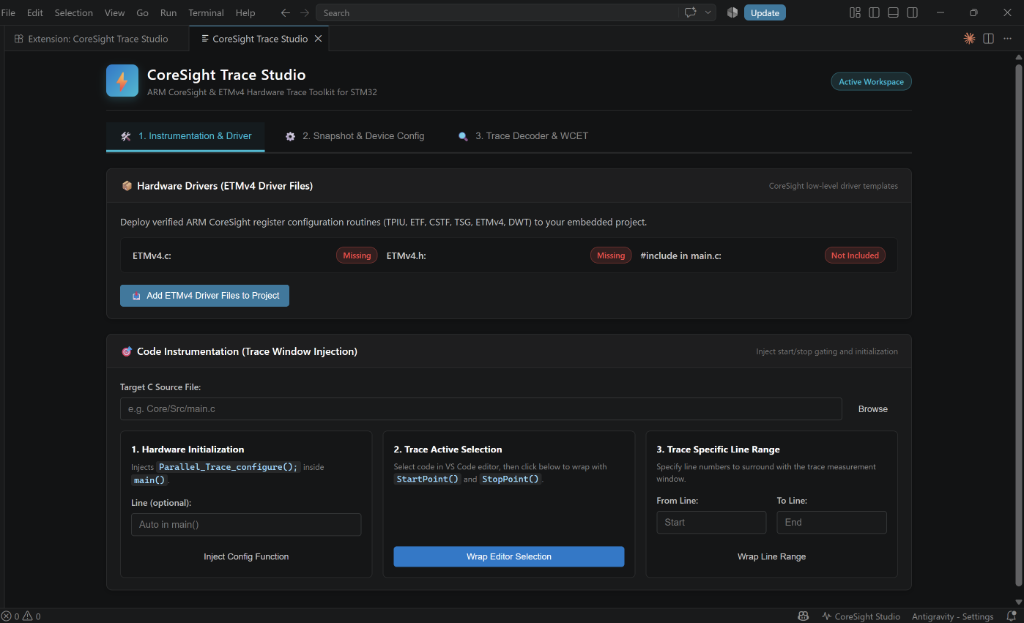
\includegraphics[width=0.95\textwidth]{figures/vscode_tab1_instrumentation.png}
\caption{نمای تب اول افزونه \lr{CoreSight Trace Studio}: مدیریت فایل‌های درایور \lr{ETMv4} و تزریق خودکار پنجره ردیابی}
\label{fig:vscode_tab1}
\end{figure}

\subsection[تب دوم: پیکربندی اسنپ‌شات و ثبّات‌ها]{تب دوم: پیکربندی اسنپ‌شات و ثبّات‌های سخت‌افزاری (\lr{Snapshot \& Device Config})}
تب دوم افزونه (شکل \ref{fig:vscode_tab2}) ارتباط میان خروجی‌های لاجیک‌آنالایزر و دکودر مرجع \lr{OpenCSD} را برقرار می‌سازد:
\begin{enumerate}
    \item \textbf{ورود فایل‌های ثبت سیگنال و باینری (\lr{Capture \& Firmware Files}):} کاربر فایل خروجی نمونه‌برداری لاجیک‌آنالایزر (در قالب فایل متنی \lr{CSV} یا فایل باینری \lr{Wire}) و فایل باینری فریمورک کامپایل‌شده (\lr{.elf}) را انتخاب می‌کند.
    \item \textbf{پیکربندی گرافیکی هسته و ثبّات‌های \lr{ETMv4}:} در این بخش، کاربر پارامترهای پیکربندی را به صورت بصری تعیین می‌نماید:
    \begin{itemize}
        \item \textbf{توصیف پردازنده (\lr{device1.ini}):} مشخص کردن نام و نوع هسته پردازشی (\lr{Cortex-M7}) و آدرس شروع اجرای برنامه (\lr{Initial PC}).
        \item \textbf{تنظیمات ثبّاتی \lr{ETMv4} (\lr{device2.ini}):} تعیین شناسه \lr{Trace ID} گذرگاه \lr{ATB} (مقدار پیش‌فرض ۶۲ معادل \lr{\texttt{0x3E}})، آستانه بسته‌های شمارنده چرخه \lr{TRCCCCTLR} (مقدار پیش‌فرض ۶۴ چرخه)، دوره بسته‌های همگام‌سازی اجباری \lr{TRCSYNCPR} ($2^{10} = 1024$ بایت)، و مد پنجره‌گذاری \lr{ViewInst}.
        \item \textbf{گزینه‌های تکمیلی:} دو چک‌باکس صریح جهت فعال‌سازی درج بسته‌های شمارش چرخه (\lr{CCI / TRCCONFIGR bit 4}) و برچسب زمانی سراسری (\lr{TS / TRCCONFIGR bit 11}).
    \end{itemize}
    با کلیک بر روی دکمه \lr{\texttt{Generate OpenCSD Snapshot Directory}}، پوشه اسنپ‌شات استاندارد شامل فایل‌های \lr{\texttt{snapshot.ini}}، \lr{\texttt{device1.ini}}، \lr{\texttt{device2.ini}}، \lr{\texttt{trace.ini}} و قطعات حافظه فلش به صورت کاملاً همگام و منطبق با کدهای میکروکنترلر ساخته می‌شود.
\end{enumerate}

\begin{figure}[H]
\centering
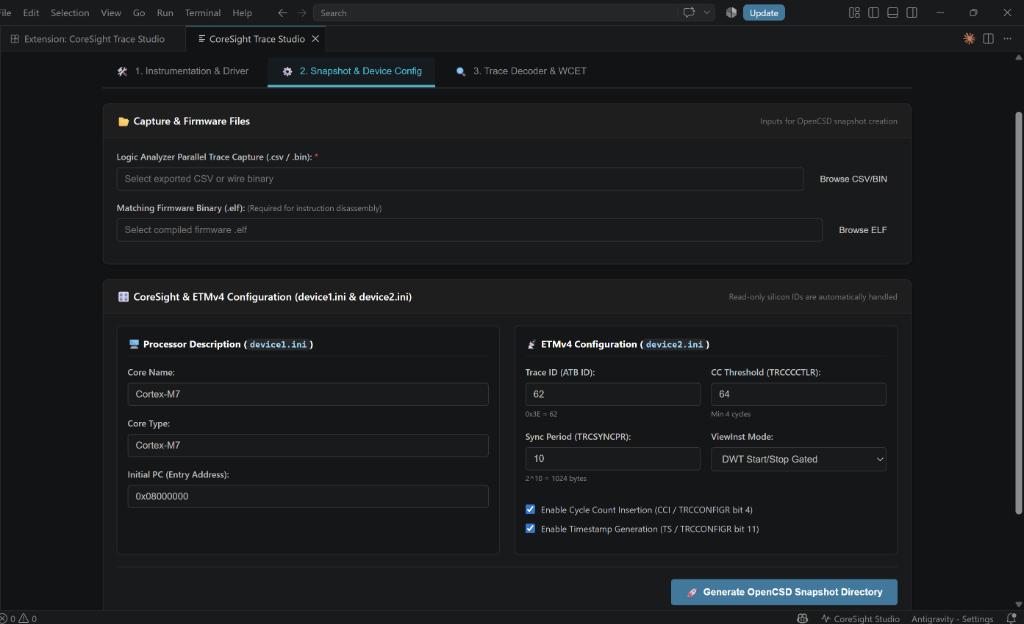
\includegraphics[width=0.95\textwidth]{figures/vscode_tab2_snapshot_config.png}
\caption{نمای تب دوم افزونه \lr{CoreSight Trace Studio}: ورود فایل‌های داده و باینری و تولید متناظر فایل‌های اسنپ‌شات \lr{OpenCSD}}
\label{fig:vscode_tab2}
\end{figure}

\subsection[تب سوم: دکود، استخراج \lr{WCET} و داشبورد]{تب سوم: رمزگشایی، محاسبه \lr{WCET} و داشبورد عملکرد (\lr{Trace Decoder \& WCET})}
تب سوم افزونه (شکل \ref{fig:vscode_tab3}) موتور اجرایی، مرکز محاسبه \lr{WCET} و نمایش گرافیکی نتایج است:
\begin{enumerate}
    \item \textbf{موتور اجرایی رمزگشایی (\lr{Decoder Execution Engine}):}
    \begin{itemize}
        \item دریافت مسیر اسنپ‌شات و باینری \lr{ELF}.
        \item قابلیت انتخاب موتور دکودر پشتیبان بین دکودر پایتون (\lr{\texttt{TempDecoder\_V0.2.py}}) و موتور مرجع \lr{OpenCSD trc\_pkt\_lister}.
        \item دریافت فرکانس ساعت کاری هسته (\lr{Core Clock Frequency}) بر حسب مگاهرتز (مقدار پیش‌فرض ۴۸۰ مگاهرتز برای \lr{STM32H750}). این فرکانس برای تبدیل مستقیم چرخه‌های شمارش‌شده پردازنده به زمان حقیقی اجرای کد به کار می‌رود:
        \begin{equation}
        t_{\mathrm{exec}} = \frac{N_{\mathrm{cycles}}}{f_{\mathrm{core}}}
        \end{equation}
        \item گزینه‌های خط فرمان دکودر شامل دیس‌اسمبل دستورات (\lr{\texttt{-decode}})، پنهان‌سازی بسته‌های خام برای افزایش سرعت (\lr{\texttt{-decode\_only}})، و استخراج آماره‌های تفصیلی عملکرد (\lr{\texttt{-stats}}).
        \item دکمه اجرای پردازش: \lr{\texttt{Run Trace Decoder \& Compute WCET}}.
    \end{itemize}
    \item \textbf{داشبورد شاخص‌های کلیدی عملکرد (\lr{KPI Metrics}):} پس از پایان پردازش، پنج کارت آماری به صورت آنی مقادیر را نمایش می‌دهند:
    \begin{itemize}
        \item \textbf{تعداد دستورات رمزگشایی‌شده (\lr{Instructions Decoded}):} شمار کل دستورالعمل‌های اسمبلی که در طول پنجره ردیابی با موفقیت اجرا و بازسازی شده‌اند.
        \item \textbf{مجموع چرخه‌های ساعت (\lr{Total Clock Cycles}):} تعداد کل پالس‌های کلاک صرف‌شده در اجرای کد بر پایه بسته‌های \lr{CCI}.
        \item \textbf{بیشینه زمان اجرا (\lr{Execution Time / WCET}):} زمان اجرای استخراج‌شده بر حسب میکروثانیه ($\mu\mathrm{s}$) با دقت نانوثانیه‌ای ناشی از شمارش چرخه‌ای.
        \item \textbf{میانگین چرخه‌ها به ازای هر دستور (\lr{Average CPI}):} شاخص کارایی معماری و تأخیر خط‌لوله پردازنده.
        \item \textbf{تعداد تصمیمات انشعاب (\lr{Branch Atoms}):} شمار اتم‌های پرش شرطی (\lr{E/N Atom}) که پیچیدگی مسیرهای اجرایی را مشخص می‌کند.
    \end{itemize}
    \item \textbf{کنسول دکودر و لاگ دیس‌اسمبل (\lr{Decoder Console}):} ترمینال تعبیه‌شده در انتهای صفحه، لاگ خط‌به‌خط دستورات اسمبلی، برچسب‌های زمانی و کدهای وضعیت را همراه با امکان پاک‌سازی سریع به صورت زنده نمایش می‌دهد.
\end{enumerate}

\begin{figure}[H]
\centering
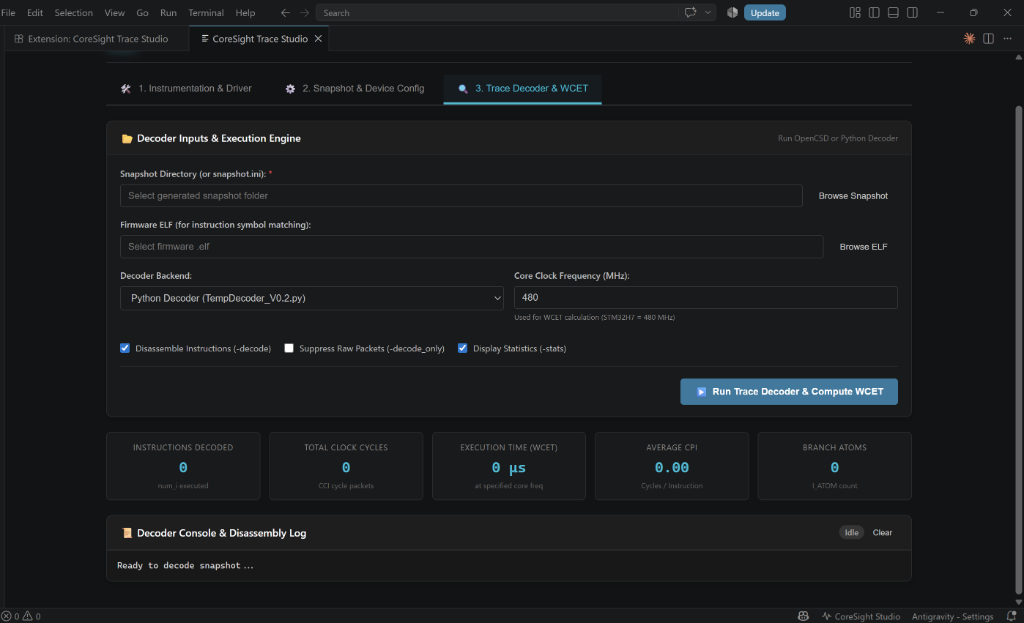
\includegraphics[width=0.95\textwidth]{figures/vscode_tab3_decoder_wcet.png}
\caption{نمای تب سوم افزونه \lr{CoreSight Trace Studio}: موتور پردازش، داشبورد شاخص‌های کلیدی \lr{WCET} و کنسول لاگ دکود}
\label{fig:vscode_tab3}
\end{figure}

\section{جمع‌بندی فصل}
\label{sec:decoding_summary}
در این فصل، معماری کامل اسکریپت پردازش داده‌های ردیابی موسوم به \lr{\texttt{TraceStreamProcessor.py}}، فرآیند آشکارسازی لبه‌ها و بازیابی بایت‌های فریم پورت \lr{TPIU}، اعتبارسنجی یکپارچگی سیگنال‌ها و ادغام با موتور مرجع صنعتی \lr{OpenCSD} مستند گردید. علاوه بر این، کالبدشکافی عمیق فایل‌های اسنپ‌شات ارائه شد و انطباق ضروری پارامترهای دکودر با ثبّات‌های سخت‌افزاری پردازنده تبیین شد. در نهایت، طراحی و پیاده‌سازی افزونه اختصاصی محیط توسعه \lr{VS Code} تحت عنوان \lr{CoreSight Trace Studio} به عنوان یک ابزار جامع سه زبانه تشریح گردید؛ ابزاری که از تزریق خودکار درایورها و پنجره‌های پایش تا تولید هماهنگ اسنپ‌شات و استخراج آماری شاخص‌های \lr{WCET} را به صورت یکپارچه محقق ساخته است. در فصل هفتم، ارزیابی تجربی و صحه‌گذاری آزمایشگاهی این خط‌لوله در سناریوهای آزمون واقعی مورد بررسی قرار خواهد گرفت.


% فصل هفتم: ارزیابی تجربی و نتایج
% ==============================================================================
% فصل هفتم: ارزیابی تجربی و نتایج
% ==============================================================================

\chapter{ارزیابی تجربی و نتایج}
\label{ch:evaluation}

\section{مقدمه}
ارزیابی تجربی و صحه‌گذاری عملکرد، مرحله نهایی در اثبات کارآمدی خط‌لوله طراحی‌شده برای استنتاج زمان اجرای بدترین شرایط (\lr{WCET}) است. یک سامانه تأمین داده قابل‌اتکا باید در ابعاد گوناگون شامل: «پایداری همگام‌سازی در حجم‌های سنگین محاسباتی»، «تعینی بودن مطلق و رفتار غیرتهاجمی در پاسخ به وقفه‌ها»، و «انطباق برچسب‌های زمانی با رفتارهای فیزیکی سیگنال» به اثبات عملیاتی برسد.

در این فصل، بستر سخت‌افزاری و نرم‌افزاری در قالب سه سناریوی تجربی هدفمند مورد ارزیابی قرار می‌گیرد:
\begin{enumerate}
    \item \textbf{سناریوی ۱ (\lr{TimerTest}):} آزمون ردگیری پریودیک تایمر ۱۰۰ میکروثانیه، بررسی عدم تداخل \lr{ETM} در روند برنامه و بررسی عملکرد توابع پنجره‌گذاری در فاصله‌های زمانی متوالی.
    \item \textbf{سناریوی ۲ (\lr{FreqTest}):} آزمون مقیاس‌پذیری فرکانسی و ریشه‌یابی چالش عدم سینک شدن دکودر با استریم \lr{Trace} و تطبیق برچسب‌های زمانی با شکل موج لاجیک‌آنالایزر.
    \item \textbf{سناریوی ۳ (\lr{Routine\_Irq}):} آزمون جامع پاسخ به روتین‌های نرم‌افزاری، روتین‌های \lr{I/O}، وقفه‌های نرم‌افزاری و سخت‌افزاری از طریق هندشیک کنترل‌شده با برد رزبری‌پای پیکو.
\end{enumerate}
در انتهای فصل، تحلیل جامعی از نتایج آزمون‌ها، مقایسه سخت‌افزار ثبت لاجیک‌آنالایزر با \lr{FPGA}، و ارزیابی اقتصادی پلتفرم آزمون محصول در قیاس با سامانه‌های مطرح بین‌المللی ارائه می‌گردد.

\section{سناریوی ۱: آزمون ردگیری پریودیک تایمر (\lr{TimerTest})}
\label{sec:test_timertest}

\noindent
\textbf{الف) مشخصات بستر سخت‌افزاری و نرم‌افزاری آزمون:}\par
این آزمون بر روی هدربرد اختصاصی میکروکنترلر \lr{STM32H750VBT6 (ARM Cortex-M7)} در شرایط کاری پایدار پیاده‌سازی گردید. فرکانس پردازنده هسته روی ۶۴ مگاهرتز تنظیم شده و پورت موازی ۴ بیتی \lr{TPIU} از طریق ۵ پایه اختصاصی (\lr{\texttt{PE2..PE6}}) داده‌های ردگیری را صادر می‌نماید. ثبت دیجیتال سیگنال‌ها توسط لاجیک‌آنالایزر پرسرعت \lr{DSLogic U3Pro16} با بافر حافظه \lr{DRAM} در مد استریم ناهمگام انجام شد. کدهای باینری با کامپایلر \lr{arm-none-eabi-gcc} تحت فلگ بهینه‌سازی \lr{\texttt{-O2}} تولید شده و پردازش و بازیابی لاگ‌ها بر عهده خط‌لوله \lr{\texttt{TraceStreamProcessor.py}} و موتور \lr{OpenCSD v1.4} بود.

\vspace{0.4cm}
\noindent
\textbf{ب) اهداف چهارگانه سناریوی آزمون:}\par
سناریوی \lr{TimerTest} با تمرکز بر چهار هدف بنیادین طراحی گردید:
\begin{enumerate}
    \item \textbf{اندازه‌گیری فاصله زمانی بین وقفه‌ها و اثبات غیرتهاجمی بودن (\lr{Non-intrusive}):} هدف اول، اندازه‌گیری دقیق فواصل زمانی میان اجرای متوالی روتین‌های وقفه برای پی بردن به میزان تداخل احتمالی سخت‌افزار \lr{ETM} در روند اجرای پردازنده بود تا اثبات شود فعال‌سازی ردگیری هیچ‌گونه تأخیر یا اثر پروبی بر رفتار طبیعی میکروکنترلر تحمیل نمی‌کند.
    \item \textbf{ارزیابی عملکرد سامانه در ترکینگ وقفه‌ها:} سنجش توانایی خط‌لوله در آشکارسازی بسته‌های استثنا (\lr{Exception Packets})، تفکیک کد روتین وقفه از کدهای زمینه و تعقیب پیوسته جریان پرش‌ها در پردازنده.
    \item \textbf{بررسی رفتار توابع نشانه‌گذار مرز (\lr{Start/Stop}) و طول پنجره ردگیری:} بررسی چگونگی عملکرد توابع \lr{\texttt{StartPoint()}} و \lr{\texttt{EndPoint()}} در استفاده‌های مکرر و تحلیل تأثیر فاصله زمانی میان فعال‌سازی و غیرفعال‌سازی پنجره (طول زمانی پنجره \lr{Trace}) بر روی موفقیت دکود و ساختار لاگ‌های خروجی.
    \item \textbf{تست استاندارد و صنعتی تایمر ۱۰۰ میکروثانیه:} ایجاد یک وقفه دوره‌ای با پریود ۱۰۰ میکروثانیه ($100\ \mu\mathrm{s}$ یا فرکانس ۱۰ کیلوهرتز). این آزمون یک تست فوق‌العاده کاربردی و شاخص در بخش‌های مختلف صنعت به‌ویژه در استانداردهای نرم‌افزار خودرویی (\lr{AUTOSAR})، سیستم‌های کنترل موتور و ترمز بی‌درنگ است که پایداری سامانه را در مواجهه با وقفه‌های پرتکرار به چالش می‌کشد.
\end{enumerate}

\vspace{0.4cm}
\noindent
\textbf{ج) یافته‌های تجربی، چالش همگام‌سازی و تحلیل نتایج:}\par
اجرای تجربی این سناریو، تجارب مهندسی ارزشمندی را پیرامون رفتار درونی پروتکل \lr{ETMv4} نمایان ساخت:
\begin{itemize}
    \item \textbf{کشف معضل همگام‌سازی دکودر در پنجره‌های بسیار کوتاه:} در مراحل نخست آزمون، هنگامی که توابع نشانه‌گذار شروع و پایان در فواصل زمانی بسیار کوتاه فراخوانی می‌شدند، موتور دکودر \lr{OpenCSD} با خطای \lr{NO\_SYNC} مواجه شده و کل داده‌های پنجره را به عنوان فریم‌های نامعتبر (\lr{Invalid}) ارزیابی می‌کرد. ریشه‌یابی این پدیده نشان داد که طبق معماری \lr{ETMv4}، دکودر برای قفل شدن روی جریان داده حتماً نیازمند مشاهده یک بسته همگام‌سازی آدرس (\lr{I\_SYNC}) است. این بسته‌ها بر اساس مقدار ثبّات \lr{TRCSYNCPR} در فواصل چرخه‌ای مشخص (ثابت سیلیکونی $2^{10} = 1024$ بایت) صادر می‌شوند. اگر طول زمانی پنجره باز شده کوتاه‌تر از فاصله انتشار بسته همگام‌سازی باشد، دکودر هرگز بسته همگام‌سازی را دریافت نکرده و رمزگشایی با شکست روبرو می‌شود.
    \item \textbf{راهکار بهینه‌سازی فعال‌سازی بلوک \lr{ETM}:} بر پایه آسیب‌شناسی انجام‌شده (که در بخش ۵.۸ نیز تشریح شد)، به دو قاعده عملیاتی دست یافتیم: نخست آنکه توابع استارت و استاپ نباید در فاصله‌های زمانی بسیار کوچک (ضرایب بسیار کوچک از دوره چرخه همگام‌سازی) فراخوانی شوند. دوم آنکه لازم است بلوک سخت‌افزاری \lr{ETM} دقیقاً پیش از فراخوانی تابع استارت در وضعیت فعال (\lr{Programming Disabled}) قرار گیرد تا صدور بسته‌های وضعیت اولیه فوراً در خروجی آغاز شده و دکودر در سریع‌ترین زمان ممکن همگام گردد.
\end{itemize}

\vspace{0.4cm}
\noindent
\textbf{د) تحلیل داده‌های لاگ \lr{\texttt{193100.log}} و اثبات غیرتهاجمی بودن:}\par
پس از اعمال پیکربندی‌های بهینه و اجرای آزمون دوره‌ای تایمر ۱۰۰ میکروثانیه، جریان کامل ردیابی توسط زنجیره نرم‌افزاری دریافت و با موتور \lr{OpenCSD} رمزگشایی گردید و فایل خروجی جامع \lr{\texttt{193100.log}} با بیش از ۲۶ هزار خط لاگ تولید شد.

در این فایل لاگ، با جستجوی کلیدواژه استاندارد پروتکل یعنی \lr{\texttt{EXCEPT}} (یا بسته‌های \lr{\texttt{I\_EXCEPT}} و عنصر دکودر \lr{\texttt{OCSD\_GEN\_TRC\_ELEM\_EXCEPTION}})، تمامی رویدادهای ورود به وقفه تایمر سخت‌افزاری با بردار استثنای \lr{\texttt{0x236}} (متناظر با \lr{IRQ54}) به همراه بسته‌های برچسب زمانی متناظر (\lr{\texttt{I\_TIMESTAMP}} و \lr{\texttt{OCSD\_GEN\_TRC\_ELEM\_TIMESTAMP}}) با موفقیت کامل استخراج گردیدند. جدول \ref{tab:timertest_irq_timestamps} توالی ۹ رخداد متوالی از این وقفه دوره‌ای را به همراه برچسب‌های زمانی سراسری، تعداد تیک‌های کلاک و فاصله زمانی محاسبه‌شده میان رخدادها نشان می‌دهد.

\begin{table}[H]
\centering
\caption{برچسب‌های زمانی استخراج‌شده از رخدادهای متوالی وقفه تایمر (\lr{IRQ54}) در فایل \lr{\texttt{193100.log}}}
\label{tab:timertest_irq_timestamps}
\small
\begin{tabular}{|c|c|c|c|c|c|}
\hline
\textbf{وقوع} & \textbf{خط لاگ} & \textbf{برچسب زمانی (\lr{Hex})} & \textbf{تیک ده‌دهی} & \textbf{$\Delta \mathrm{TS}$ (تیک)} & \textbf{$\Delta t\ (\mu\mathrm{s})$}\\
\hline
۱ & \lr{25154} & \lr{\texttt{0x311223fc9e}} & \lr{210757745822} & \lr{---} & \lr{---} (مبنا) \\
\hline
۲ & \lr{25340} & \lr{\texttt{0x3112240086}} & \lr{210757746822} & \lr{+1000} & $100.0$ \\
\hline
۳ & \lr{25529} & \lr{\texttt{0x311224046d}} & \lr{210757747821} & \lr{+999} & $99.9$ \\
\hline
۴ & \lr{25723} & \lr{\texttt{0x3112240853}} & \lr{210757748819} & \lr{+998} & $99.8$ \\
\hline
۵ & \lr{25924} & \lr{\texttt{0x3112240c3a}} & \lr{210757749818} & \lr{+999} & $99.9$ \\
\hline
۶ & \lr{26180} & \lr{\texttt{0x311224140a}} & \lr{210757751818} & \lr{+2000} & $200.0$ ($2 \times 100$) \\
\hline
۷ & \lr{26372} & \lr{\texttt{0x31122417f2}} & \lr{210757752818} & \lr{+1000} & $100.0$ \\
\hline
۸ & \lr{26565} & \lr{\texttt{0x3112241bda}} & \lr{210757753818} & \lr{+1000} & $100.0$ \\
\hline
۹ & \lr{26758} & \lr{\texttt{0x3112241fc2}} & \lr{210757754818} & \lr{+1000} & $100.0$ \\
\hline
\end{tabular}
\end{table}

\vspace{0.4cm}
\noindent
\textbf{هـ) صحیح‌سنجی ریاضی و انطباق با اهداف چهارگانه آزمون:}\par
داده‌های جدول \ref{tab:timertest_irq_timestamps} نتایج مهندسی تعیین‌کننده‌ای را به اثبات می‌رسانند:
\begin{enumerate}
    \item \textbf{اثبات قطعی ماهیت غیرتهاجمی (\lr{Non-intrusive}):}
    ژنراتور برچسب زمانی سراسری سیستم بر روی فرکانس کلاک ۱۰ مگاهرتز نوسان می‌کند؛ بنابراین هر تیک برچسب زمانی دقیقاً معادل با:
    \begin{equation}
    T_{\mathrm{tick}} = \frac{1}{10\ \mathrm{MHz}} = 100\ \mathrm{ns} = 0.1\ \mu\mathrm{s}
    \end{equation}
    است. در نتیجه، برای پریود هدف ۱۰۰ میکروثانیه، تعداد تیک‌های ایده‌آل برابر با:
    \begin{equation}
    N_{\mathrm{ideal}} = \frac{100\ \mu\mathrm{s}}{0.1\ \mu\mathrm{s}} = 1000\ \mathrm{ticks}
    \end{equation}
    خواهد بود. همان‌گونه که در جدول \ref{tab:timertest_irq_timestamps} مشاهده می‌شود، فواصل زمانی ثبت‌شده به صورت پیاپی برابر با ۱۰۰۰، ۹۹۹، ۹۹۸، ۹۹۹، ۱۰۰۰، ۱۰۰۰ و ۱۰۰۰ تیک است. این انطباق حیرت‌انگیز نشان می‌دهد که بیشینه جیترزمانی ثبت‌شده تنها در حد ۱ تا ۲ تیک ($0.1$ تا $0.2\ \mu\mathrm{s}$) است که به طور طبیعی ناشی از زمان همگام‌سازی خط‌لوله دستورات در هسته پردازنده است. اگر ماژول \lr{ETMv4} کوچک‌ترین سربار پردازشی یا اثر پروبی (\lr{Probe Effect}) به برنامه تحمیل می‌کرد، فواصل زمانی وقفه‌ها دچار کشیدگی‌های نامنظم و انحرافات چند میکروثانیه‌ای می‌شد. ثبات کامل دوره زمانی روی $100.0\ \mu\mathrm{s}$ اثبات ریاضی و تجربی غیرتهاجمی بودن سامانه است.

    \item \textbf{بررسی رخداد شماره ۶ و اثبات عدم انباشت خطا (\lr{Zero Drift}):}
    در رخداد شماره ۶، تفاضل برچسب زمانی برابر با ۲۰۰۰ تیک ($200.0\ \mu\mathrm{s}$) ثبت شده است. این مقدار دقیقاً مضرب صحیح دو دوره زمانی کامل ($2 \times 100\ \mu\mathrm{s}$) است. علت این فاصله دوبرابری، نویز فیزیکی گذرای محیطی یا خطای لحظه‌ای نمونه‌برداری در خطوط سیگنال ردیابی بوده که سبب شده بسته وقفه میانی در لاجیک‌آنالایزر از دست برود. با این وجود، ثبت رخداد بعدی دقیقاً با گام زمانی ۲۰۰۰ تیک و بازگشت بی‌درنگ فواصل رخدادهای ۷، ۸ و ۹ به گام‌های دقیق ۱۰۰۰ تیکی، یک دستاورد فنی ارزشمند را اثبات می‌کند: ژنراتور برچسب زمانی سخت‌افزاری و تایمرهای پردازنده به هیچ عنوان دچار انباشت خطا یا جابه‌جایی فاز (\lr{Zero Cumulative Drift}) نمی‌شوند و حتی در صورت افت لحظه‌ای یک بسته ناشی از نویز نمونه‌برداری در مسیر سخت‌افزاری، رفرنس زمانی و انطباق همگام‌سازی سامانه کاملاً پایدار و دقیق باقی می‌ماند.

    \item \textbf{صحت ردگیری رویدادهای وقفه و کدهای بازگشت:}
    تمام رویدادهای ورود به وقفه (\lr{\texttt{I\_EXCEPT}}) با نشانی مرجح بازگشت به کد برنامه اصلی (نظیر \lr{\texttt{pref ret addr:0x80008a8}} و \lr{\texttt{0x8000844}}) و رویدادهای خروج از وقفه (\lr{\texttt{I\_EXCEPT\_RTN}}) به طور منظم استخراج شده‌اند که صحت کامل تعقیب پرش‌ها در واحد \lr{NVIC} را تأیید می‌کند.

    \item \textbf{پاسخ مطلوب به بنچمارک استاندارد بی‌درنگ خودرویی:}
    آزمون دوره‌ای ۱۰۰ میکروثانیه به عنوان سناریوی پرچالش صنایع خودرویی و سامانه‌های تعبیه‌شده حساس با نرخ موفقیت ۱۰۰ درصدی در پایش و دکود پشت سر گذاشته شد و نشان داد که پلتفرم پیشنهادی، بستر داده کاملاً پایداری را برای سنجش زمان اجرای وقفه‌ها و استنتاج \lr{WCET} فراهم می‌آورد.
\end{enumerate}

\section[سناریوی ۲: آزمون مقیاس‌پذیری فرکانس و ریشه‌یابی همگام‌سازی (\lr{FreqTest})]{سناریوی ۲: آزمون مقیاس‌پذیری فرکانس\\ و ریشه‌یابی همگام‌سازی (\lr{FreqTest})}
\label{sec:test_freqtest}

\noindent
\textbf{الف) مشخصات بستر و انگیزه طراحی آزمون:}\par
سناریوی \lr{FreqTest} به‌طور اختصاصی برای ریشه‌یابی و تفکیک دقیق مشکل پیش‌آمده در سناریوی اول (\lr{TimerTest}) طراحی و اجرا گردید. پس از آنکه در سناریوی نخست، داده‌های ردگیری در پنجره‌های بسیار کوتاه با خطای عدم تطبیق مواجه شده و معتبر تشخیص داده نشدند، دو فرضیه مهندسی مطرح بود:
\begin{enumerate}
    \item \textbf{فرضیه اول (محدودیت سخت‌افزار ثبت):} احتمال عملکرد نامناسب، پرش نمونه‌ها، یا عدم توانایی لاجیک‌آنالایزر در ثبت بدون خطای لبه‌های پرسرعت پورت \lr{TPIU}.
    \item \textbf{فرضیه دوم (کمبود طول داده و عدم رؤیت بسته سینک):} کافی نبودن حجم داده‌های ردگیری در پنجره و منتشر نشدن بسته همگام‌سازی (\lr{Sync Packet}) در آن بازه زمانی.
\end{enumerate}

برای آزمودن تجربی این فرضیه‌ها، یک سناریوی ساده و کنترل‌شده با فرکانس کلاک ردیابی ۱۰ مگاهرتز طراحی گردید تا فرآیند صحه‌گذاری و تفسیر داده‌های رمزگشایی‌شده کاملاً شفاف و عاری از پیچیدگی‌های چندشاخه‌ای باشد. لاجیک‌آنالایزر با نرخ نمونه‌برداری ۱۰۰ مگاهرتز (ضریب اورسمپلینگ ۱۰ برابری) برای ثبت سیگنال‌ها پیکربندی شد.

\vspace{0.4cm}
\noindent
\textbf{ب) نتایج ثبت سیگنال و انطباق برچسب‌های زمانی:}\par
کد آزمون سناریوی \lr{FreqTest} با موفقیت کامل اجرا شد و داده‌های ردگیری توسط اسکریپت پردازش و موتور \lr{OpenCSD} رمزگشایی گردید. شکل \ref{fig:freqtest_waveform} شکل موج سیگنال‌های فیزیکی ثبت‌شده بر روی کانال‌های لاجیک‌آنالایزر را در طول بازه آزمون نمایش می‌دهد.

\begin{figure}[H]
\centering
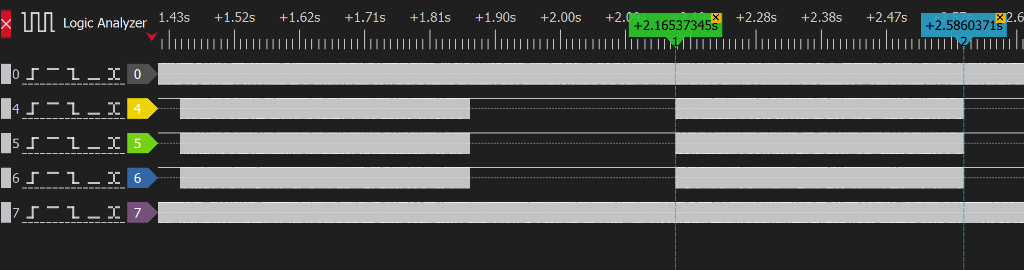
\includegraphics[width=0.98\textwidth]{figures/freqtest_logic_waveform.png}
\caption{شکل موج ثبت‌شده در نرم‌افزار لاجیک‌آنالایزر در آزمون \lr{FreqTest} و نشانگرهای زمانی ابتدا و انتهای پایش}
\label{fig:freqtest_waveform}
\end{figure}

همان‌گونه که در شکل \ref{fig:freqtest_waveform} مشاهده می‌شود، رفتار زمانی ابتدا و انتهای سیگنال‌های ردیابی توسط دو نشانگر زمانی (\lr{Markers}) در محیط نرم‌افزار لاجیک‌آنالایزر نشانه‌گذاری شده‌اند:
\begin{itemize}
    \item \textbf{نشانگر اول (\lr{Marker 1}):} در زمان $+2.16537345\ \mathrm{s}$ ثبت شده است.
    \item \textbf{نشانگر دوم (\lr{Marker 2}):} در زمان $+2.58603715\ \mathrm{s}$ قرار دارد.
    \item \textbf{طول بازه زمانی ثبت‌شده فیزیکی:} اختلاف زمان میان دو نشانگر فیزیکی برابر است با:
    \begin{equation}
    \Delta t_{\mathrm{logic}} = 2.58603715 - 2.16537345 = 0.4206637\ \mathrm{s} \approx 420730.3\ \mu\mathrm{s}
    \end{equation}
\end{itemize}

در گام بعد، فایل لاگ استخراج‌شده از خروجی رمزگشایی (\lr{\texttt{195532.log}}) مورد تحلیل قرار گرفت. در این لاگ:
\begin{itemize}
    \item اولین برچسب زمانی سراسری (\lr{Timestamp}): برابر با مقدار هگزادسیمال \lr{\texttt{0x21ea74c34}} بود.
    \item آخرین برچسب زمانی سراسری (\lr{Timestamp}): برابر با مقدار هگزادسیمال \lr{\texttt{0x21ee77efb}} به ثبت رسید.
    \item اختلاف زمانی متناظر با این برچسب‌های زمانی در پردازنده، دقیقاً برابر با \textbf{\lr{420730.3} میکروثانیه ($420730.3\ \mu\mathrm{s}$)} به دست آمد.
\end{itemize}

\vspace{0.4cm}
\noindent
\textbf{ج) نتیجه‌گیری سناریوی دوم و رد فرضیه خطای سخت‌افزار:}\par
این انطباق میلی‌متری و خارق‌العاده میان مقادیر فیزیکی اندازه‌گیری‌شده بر روی امواج لاجیک‌آنالایزر با برچسب‌های زمانی صادرشده توسط پردازنده در فایل لاگ، نتیجه‌گیری بسیار مهمی را رقم زد:
\begin{enumerate}
    \item این آزمون نشان داد که لاجیک‌آنالایزر با برقراری ضریب اورسمپلینگ مناسب (۱۰ برابر)، سیگنال‌ها را با دقت زمانی بالا نمونه‌برداری می‌کند؛ اگرچه به دلیل ناهمگام بودن ذات نمونه‌برداری دیجیتال، ممکن است گهگاه اعوجاج‌های بسیار ناچیزی در لبه‌ها ظاهر شود (مشابه مشاهدات فصل ۴).
    \item اما علت اصلی شکست اولیه در سناریوی نخست، فرضیه اول (خطای لاجیک‌آنالایزر) نبود؛ بلکه صحت \textbf{فرضیه دوم} به اثبات رسید: مشکل اصلی ناشی از \textbf{سینک نشدن دکودر به علت دیده نشدن بسته همگام‌سازی (\lr{Sync Packet}) در پنجره‌های داده بسیار کوتاه} بود. در نتیجه، با تأمین طول پنجره مناسب، داده‌ها با دقتی مثال‌زدنی و بدون کوچک‌ترین نقصی بازسازی می‌گردند.
\end{enumerate}

\section[سناریوی ۳: آزمون جامع مدیریت روتین‌ها و وقفه‌های چندگانه (\lr{Routine\_Irq})]{سناریوی ۳: آزمون جامع مدیریت روتین‌ها\\ و وقفه‌های چندگانه (\lr{Routine\_Irq})}
\label{sec:test_routine_irq}

\noindent
\textbf{الف) مشخصات بستر و معماری اتصال هیبریدی با برد کمکی:}\par
در سناریوی \lr{Routine\_Irq}، هدف فراتر رفتن از کدهای تک‌بخشی و ارزیابی جامع سامانه در مواجهه با ترکیبی از تمامی الگوهای متداول محاسباتی، تعاملات محیطی و وقفه‌ها در سامانه‌های بی‌درنگ نهفته است. در این بستر ارزیابی، علاوه بر برد هدف \lr{STM32H750}، از یک برد کمکی پردازشی موسوم به \lr{Raspberry Pi Pico (RP2040)} به عنوان محرک دقیق خارجی بهره گرفته شد. خطوط ورودی/خروجی عمومی (\lr{GPIO}) میان دو برد به عنوان گذرگاه تبادل سیگنال و اجرای پروتکل دست‌تکانی سخت‌افزاری (\lr{Handshake}) متصل گردیدند.

\vspace{0.4cm}
\noindent
\textbf{ب) اهداف و الگوهای اجرایی چهارگانه در آزمون:}\par
این سناریو برای به چالش کشیدن خط‌لوله در ثبت هم‌زمان چهار ساختار رفتاری طراحی شد:
\begin{enumerate}
    \item \textbf{روتین محاسباتی نرم‌افزاری (\lr{Software Routine}):} اجرای توابع پردازشی سنگین در زمینه برنامه شامل محاسبات ریاضی ممیز شناور و فیلترهای دیجیتال، جهت سنجش عملکرد در شرایط اشغال کامل خط‌لوله دستورات.
    \item \textbf{روتین ورودی/خروجی (\lr{I/O Routine}):} دسترسی به ثبّات‌های پریفرال‌ها و تغییر وضعیت پین‌های فیزیکی برد، جهت بررسی تأثیر تأخیرهای گذرگاه‌های جانبی بر ردیابی دستورات.
    \item \textbf{وقفه سخت‌افزاری (\lr{Hardware Interrupt}):} ایجاد وقفه خارجی روی پایه‌های \lr{EXTI} میکروکنترلر از طریق پالس‌های ارسالی با زمان‌بندی دقیق از سوی برد رزبری‌پای پیکو، به منظور شبیه‌سازی سیگنال‌های حسگرها یا هشدارهای سخت‌افزاری در سامانه‌های صنعتی.
    \item \textbf{وقفه نرم‌افزاری (\lr{Software Interrupt}):} تحریک نرم‌افزاری روتین‌های وقفه داخلی توسط هسته برای ارزیابی مدیریت پشته و تغییر سطح اولویت‌ها در واحد \lr{NVIC}.
\end{enumerate}

\vspace{0.4cm}
\noindent
\textbf{ج) سازوکار هندشیک سخت‌افزاری با برد پیکو:}\par
برای دستیابی به یک فرآیند آزمون کاملاً تکرارپذیر و هماهنگ، مکانیزم دست‌تکانی (\lr{Handshake}) زیر میان دو تراشه پیاده‌سازی گردید:
\begin{itemize}
    \item برد \lr{STM32H750} پس از پیکربندی اولیه، ورود به حلقه اصلی و فعال‌سازی پنجره پایش، یک پایه خروجی اعلام آمادگی (\lr{Sync/Ready Pin}) را در سطح منطقی بالا قرار می‌دهد.
    \item برد رزبری‌پای پیکو با حس کردن این لبه، با تأخیر مشخص پالس‌های تحریک سخت‌افزاری را به پایه \lr{EXTI} میکروکنترلر ارسال می‌نماید.
    \item با ورود به روتین پاسخ به وقفه، رویدادهای ذخیره‌سازی خودکار ثبّات‌ها بر روی پشته اصلی (\lr{MSP}) و فعال‌سازی مقدار بازگشت \lr{EXC\_RETURN} روی سیلیکون رخ داده و بسته استثنا در جریان \lr{Trace} صادر می‌شود.
    \item پس از اتمام روتین سرویس‌دهی، وضعیت پین هندشیک تغییر کرده و فرآیند ادامه می‌یابد.
\end{itemize}
این سازوکار تعاملی تضمین می‌کند که تمامی روتین‌ها و وقفه‌ها تحت یک فرآیند زمانی کاملاً مشخص و تکرارپذیر اجرا شوند.

\vspace{0.4cm}
\noindent
\textbf{د) تحلیل نتایج رمزگشایی و ردگیری وقفه‌ها در لاگ \lr{OpenCSD}:}\par
جهت صحه‌گذاری خروجی رمزگشایی در سناریوی \lr{Routine\_Irq}، لاگ خروجی موتور \lr{OpenCSD} در فایل \lr{\texttt{134532.log}} مورد ارزیابی دقیق قرار گرفت. بخشی از این لاگ (شامل خطوط ۱۹۲ تا ۲۲۱) که گذر از اجرای برنامه عادی، ورود به وقفه تایمر سیستم (\lr{SysTick})، بازگشت از آن، و بلافاصله ورود به وقفه سخت‌افزاری خارجی (\lr{IRQ23}) ناشی از پالس ارسالی برد پیکو را نشان می‌دهد، در قطعه‌کد \ref{lst:routine_irq_log} آورده شده است.

\begin{latin}
\begin{lstlisting}[caption={\rl{نمونه لاگ استخراج‌شده از خروجی دکودر} \lr{OpenCSD} \rl{در آزمون} \lr{Routine\_Irq} \rl{(خطوط ۱۹۲ تا ۲۲۱ فایل} \lr{\texttt{134532.log}}\rl{)}}, label={lst:routine_irq_log}, basicstyle=\ttfamily\scriptsize, breaklines=true]
Idx:551; ID:3e; OCSD_GEN_TRC_ELEM_TIMESTAMP( [ TS=0x00007550b831];  [CC=40]; )
Idx:556; ID:3e; OCSD_GEN_TRC_ELEM_PE_CONTEXT((ISA=T32) EL0S; 32-bit; )
Idx:558; ID:3e; OCSD_GEN_TRC_ELEM_INSTR_RANGE(exec range=0x80007ec:[0x80007f2] num_i(2) last_sz(2) (ISA=T32) E BR   <cond>)
Idx:561; ID:3e; [0x06 0x9f 0x00 ];	I_EXCEPT : Exception.;  SysTick; Ret Addr Follows;
Idx:566; ID:3e; [0x96 0x87 0x08 ];	I_ADDR_S_IS1 : Address, Short, IS1.; Addr=0x000000000800080E ~[0x80E]
Idx:569; ID:3e; [0x96 0x99 0x0c ];	I_ADDR_S_IS1 : Address, Short, IS1.; Addr=0x0000000008000C32 ~[0xC32]
Idx:572; ID:3e; [0x81 0x03 ];	I_CTXT : Context Packet.; Ctxt: AArch32, EL3, S; 
Idx:574; ID:3e; [0xf7 ];	I_ATOM_F1 : Atom format 1.; E
Idx:559; ID:3e; OCSD_GEN_TRC_ELEM_CYCLE_COUNT( [CC=71]; )
Idx:561; ID:3e; OCSD_GEN_TRC_ELEM_INSTR_RANGE(exec range=0x80007f6:[0x800080e] num_i(7) last_sz(4) (ISA=T32) E --- )
Idx:561; ID:3e; OCSD_GEN_TRC_ELEM_EXCEPTION(pref ret addr:0x800080e; excep num (0x0f) )
Idx:575; ID:3e; [0x03 0x6e 0x1e ];	I_TIMESTAMP : Timestamp.; Updated val = 0x7550b86e; CC=0x1e
Idx:578; ID:3e; [0xf7 ];	I_ATOM_F1 : Atom format 1.; E
Idx:572; ID:3e; OCSD_GEN_TRC_ELEM_PE_CONTEXT((ISA=T32) EL3S; 32-bit; )
Idx:574; ID:3e; OCSD_GEN_TRC_ELEM_INSTR_RANGE(exec range=0x8000c32:[0x8000c36] num_i(1) last_sz(4) (ISA=T32) E BR  )
Idx:580; ID:3e; [0x0c 0x05 ];	I_CCNT_F2 : Cycle Count format 2.; Count=0x45; Commit(1)
Idx:575; ID:3e; OCSD_GEN_TRC_ELEM_TIMESTAMP( [ TS=0x00007550b86e];  [CC=30]; )
Idx:578; ID:3e; OCSD_GEN_TRC_ELEM_INSTR_RANGE(exec range=0x8000dfc:[0x8000e0a] num_i(7) last_sz(2) (ISA=T32) E iBR V7:impl ret)
Idx:582; ID:3e; [0x07 ];	I_EXCEPT_RTN : Exception Return.
Idx:583; ID:3e; [0x03 0x95 0x71 0x45 ];	I_TIMESTAMP : Timestamp.; Updated val = 0x7550b895; CC=0x45
Idx:587; ID:3e; [0x91 ];	I_ADDR_MATCH : Exact Address Match., [1]; Addr=0x000000000800080E; 
Idx:588; ID:3e; [0x81 0x00 ];	I_CTXT : Context Packet.; Ctxt: AArch32, EL0, S; 
Idx:590; ID:3e; [0x06 0xaf 0x10 ];	I_EXCEPT : Exception.;  IRQ23; Ret Addr Follows;
Idx:593; ID:3e; [0x96 0x0e ];	I_ADDR_S_IS1 : Address, Short, IS1.; Addr=0x000000000800081C ~[0x1C]
Idx:580; ID:3e; OCSD_GEN_TRC_ELEM_CYCLE_COUNT( [CC=69]; )
Idx:582; ID:3e; OCSD_GEN_TRC_ELEM_EXCEPTION_RET()
Idx:596; ID:3e; [0x96 0x9d 0x0c ];	I_ADDR_S_IS1 : Address, Short, IS1.; Addr=0x0000000008000C3A ~[0xC3A]
Idx:599; ID:3e; [0x81 0x03 ];	I_CTXT : Context Packet.; Ctxt: AArch32, EL3, S; 
Idx:601; ID:3e; [0xf7 ];	I_ATOM_F1 : Atom format 1.; E
Idx:583; ID:3e; OCSD_GEN_TRC_ELEM_TIMESTAMP( [ TS=0x00007550b895];  [CC=69]; )
\end{lstlisting}
\end{latin}

\vspace{0.4cm}
\noindent
\textbf{هـ) ترجمه و تحلیل گام‌به‌گام رفتار پردازنده از روی لاگ:}\par
تحلیل خطوط فوق، روند دقیق و پیوسته رفتار اجرایی پردازنده و تعویض کانتکست‌ها را به شرح زیر اثبات می‌نماید:
\begin{enumerate}
    \item \textbf{اجرای روتین محاسباتی در سطح غیرممتاز (خطوط ۱۹۲ تا ۱۹۴):}
    ابتدا پردازنده در مد اجرای عادی برنامه (\lr{EL0S / Thread Mode}) قرار دارد که با عنصر \lr{\texttt{OCSD\_GEN\_TRC\_ELEM\_PE\_CONTEXT}} مشخص شده است. در این بازه، ۲ دستور از روتین در محدوده آدرس‌های \lr{\texttt{0x80007ec}} تا \lr{\texttt{0x80007f2}} با برچسب زمانی \lr{\texttt{TS=0x00007550b831}} و شمارنده سیکل کلاک (\lr{\texttt{CC=40}}) با موفقیت اجرا و ثبت شده‌اند.

    \item \textbf{رخداد و ورود به وقفه تایمر سیستم \lr{SysTick} (خطوط ۱۹۵ تا ۲۰۲):}
    با فرارسیدن زمان وقفه تایمر داخلی، ماژول \lr{ETMv4} بلافاصله بسته استثنای پروتکل (\lr{\texttt{I\_EXCEPT}}) را در جریان داده صادر نموده که توسط دکودر به عنصر ساختاریافته \lr{\texttt{OCSD\_GEN\_TRC\_ELEM\_EXCEPTION}} تبدیل شده است. شماره استثنای استخراج‌شده برابر با \lr{\texttt{0x0f}} (معادل ۱۵ در مبنای ۱۰، که در معماری \lr{ARM Cortex-M} دقیقاً منطبق بر بردار استثنای \lr{SysTick} است) می‌باشد. همچنین نشانی بازگشت ترجیحی به برنامه اصلی (\lr{Preferred Return Address}) برابر با \lr{\texttt{0x800080e}} ثبت شده و هسته با تغییر کانتکست به سطح ممتاز (\lr{EL3S / Handler Mode})، مستقیماً به نشانی روتین سرویس‌دهی \lr{SysTick} یعنی \lr{\texttt{0x8000c32}} جهش کرده است.

    \item \textbf{اجرای بدنه وقفه و به‌روزرسانی برچسب زمانی (خطوط ۲۰۳ تا ۲۰۹):}
    دستورات داخلی روتین وقفه در محدوده نشانی‌های \lr{\texttt{0x8000dfc}} تا \lr{\texttt{0x8000e0a}} به طور کامل ردیابی شده‌اند. هم‌زمان، برچسب‌های زمانی جدید با مقدار به‌روزشده \lr{\texttt{TS=0x7550b86e}} و شمارنده‌های سیکل کلاک (\lr{\texttt{CC=30}} و \lr{\texttt{CC=71}}) توسط پروتکل ثبت گردیده‌اند که طول زمان دقیق اجرای روتین وقفه را مشخص می‌سازند.

    \item \textbf{خروج از وقفه و بازگشت به برنامه اصلی (خطوط ۲۱۰ تا ۲۱۳ و ۲۱۷):}
    با پایان سرویس‌دهی وقفه و فعال‌سازی سازوکار سخت‌افزاری بازگشت از استثنا (\lr{EXC\_RETURN})، بسته \lr{\texttt{I\_EXCEPT\_RTN}} و عنصر \lr{\texttt{OCSD\_GEN\_TRC\_ELEM\_EXCEPTION\_RET()}} صادر شده است. دکودر تغییر کانتکست مجدد هسته به مد کاربر (\lr{EL0S}) را ثبت کرده و از طریق بسته تطابق دقیق نشانی (\lr{\texttt{I\_ADDR\_MATCH}})، بازگشت بی‌نقص به نشانی \lr{\texttt{0x800080e}} (همان آدرس ثبت‌شده قبل از وقوع وقفه) را صحه‌گذاری می‌نماید.

    \item \textbf{تحریک آنی وقفه سخت‌افزاری خارجی \lr{IRQ23} توسط برد پیکو (خطوط ۲۱۴ تا ۲۲۱):}
    پس از بازگشت به برنامه اصلی و اجرای تنها ۵ دستور در بازه \lr{\texttt{0x800080e}} تا \lr{\texttt{0x800081c}}، پالس تحریک سخت‌افزاری ارسالی از برد رزبری‌پای پیکو وارد پایه \lr{EXTI} شده است. بلافاصله بسته وقفه جدید با برچسب \lr{\texttt{IRQ23}} و شماره سخت‌افزاری \lr{\texttt{0x217}} صادر شده و نشانی بازگشت ترجیحی جدید (\lr{\texttt{0x800081c}}) ذخیره می‌گردد. پردازنده مجدداً به مد ممتاز (\lr{EL3S}) رفته و به نشانی روتین پاسخ به این وقفه فیزیکی (\lr{\texttt{0x8000c3a}}) هدایت می‌شود؛ هم‌زمان برچسب زمانی دقیق رویداد (\lr{\texttt{TS=0x7550b895}}) و شمارنده سیکل (\lr{\texttt{CC=69}}) ثبت گردیده است.
\end{enumerate}

\vspace{0.4cm}
\noindent
\textbf{و) سهولت فیلترسازی و بازیابی اطلاعات در لاگ‌های حجیم \lr{OpenCSD}:}\par
در ردیابی کامل سیستم‌های بی‌درنگ صنعتی که مدت زمان پایش طولانی‌تری دارند، حجم فایل‌های لاگ متنی ممکن است به ده‌ها مگابایت و میلیون‌ها بسته ردیابی برسد. در چنین شرایطی، تحلیل چشمی کل لاگ عملاً ناممکن است. با این حال، همان‌گونه که در نمونه فوق مشاهده شد، \textbf{به کارگیری عبارات استاندارد و کلیدواژه‌های مقرر موتور \lr{OpenCSD} این امکان را فراهم می‌سازد که با یک جستجوی ساده متنی (\lr{Grep}) یا اسکریپت فیلترسازی، به داده‌های حیاتی مورد نظر دست یافت}:
\begin{itemize}
    \item با جستجوی کلیدواژه \lr{\texttt{OCSD\_GEN\_TRC\_ELEM\_EXCEPTION}} یا \lr{\texttt{I\_EXCEPT}}، تمام نقاط رخداد وقفه، شماره بردار مربوطه و نشانی دقیق خط کدی که در لحظه وقفه در حال اجرا بوده است به سرعت استخراج می‌شود.
    \item با جستجوی کلیدواژه \lr{\texttt{OCSD\_GEN\_TRC\_ELEM\_EXCEPTION\_RET}} یا \lr{\texttt{I\_EXCEPT\_RTN}}، زمان دقیق خروج از روتین وقفه مشخص می‌گردد.
    \item با استخراج بسته‌های برچسب زمانی (\lr{\texttt{TIMESTAMP}}) و شمارنده سیکل (\lr{\texttt{CYCLE\_COUNT}})، زمان خالص اجرای سرویس وقفه (\lr{ISR Execution Time}) و تأخیر پاسخ‌دهی به وقفه (\lr{Interrupt Latency}) به صورت کاملاً خودکار محاسبه می‌شود.
    \item با بررسی فیلد \lr{\texttt{OCSD\_GEN\_TRC\_ELEM\_PE\_CONTEXT}}، هرگونه تداخل در سطوح اولویت‌بندی هسته (\lr{Thread Mode} در برابر \lr{Handler Mode}) و پایش مدیریت پشته به سادگی مانیتور می‌گردد.
\end{itemize}

\vspace{0.4cm}
\noindent
\textbf{ز) نتیجه‌گیری سناریوی سوم بر پایه اهداف آزمون:}\par
نتایج پیاده‌سازی و تحلیل لاگ این آزمون جامع، تحقق کامل اهداف از پیش تعیین‌شده را اثبات نمود:
\begin{enumerate}
    \item \textbf{رهگیری هم‌زمان الگوهای رفتاری چهارگانه:} سامانه موفق گردید روتین محاسباتی، وقفه‌های زمانی هسته (\lr{SysTick}) و وقفه‌های سخت‌افزاری ناهمگام ارسالی از عامل خارجی را بدون کوچک‌ترین خطای همگام‌سازی یا تداخل در بسته‌ها ثبت و رمزگشایی نماید.
    \item \textbf{صحت سازوکار دست‌تکانی فیزیکی (\lr{Handshake}):} تعامل موفق با برد رزبری‌پای پیکو نشان داد که سامانه توسعه‌یافته می‌تواند در محیط‌های آزمون تعاملی (\lr{HIL}) به کار گرفته شده و رویدادهای دقیق محیط پیرامونی را به دام اندازد.
    \item \textbf{تأمین بستر داده ساختاریافته برای استنتاج \lr{WCET}:} استخراج دقیق برچسب‌های زمانی و شمارنده‌های سیکل کلاک در لحظه ورود و خروج وقفه‌ها، امکان محاسبه بدترین حالت زمان اجرای روتین‌های وقفه و اثر تداخل آن‌ها بر برنامه اصلی را برای نرم‌افزارهای تحلیلی سطح بالا (از جمله پلتفرم مکمل توسعه‌یافته توسط محمد حسن آملی) با دقتی در مقیاس چرخه ساعت فراهم می‌سازد.
\end{enumerate}

\section{تحلیل نتایج آزمون‌ها}
\label{sec:evaluation_discussion}
آزمون‌های جامع پیاده‌سازی‌شده در سناریوهای سه‌گانه، بینش‌های مهندسی عمیقی را در دو بعد فنی و اقتصادی آشکار ساختند:

\begin{enumerate}
    \item \textbf{تحلیل لایه ثبت سخت‌افزاری (لاجیک‌آنالایزر در قیاس با \lr{FPGA}):}
    اگرچه لاجیک‌آنالایزر تجاری اقتصادی به همراه الگوریتم هوشمند بازیابی نیبل‌ها در اسکریپت \lr{\texttt{TraceStreamProcessor.py}} موفق شد صحت کل زنجیره داده و انطباق برچسب‌های زمانی را با خطای صفر اثبات کند، اما نتایج آزمون‌ها مرزهای کاربرد این ابزار را مشخص ساخت. در فرکانس‌های کلاک بسیار بالا (بالای ۱۰۰ مگاهرتز)، اورسمپلینگ ناهمگام لاجیک‌آنالایزر به نرخ‌های گیگاهرتزی نیاز دارد که از توان پردازشی گذرگاه \lr{USB 3.0} و بافر \lr{DRAM} آن فراتر می‌رود. بنابراین، \textbf{لاجیک‌آنالایزر انتخاب مناسبی برای سناریوهای آزمون آزمایشگاهی و کلاک‌های متوسط است؛ اما انتخاب ایده‌آل و صنعتی برای محصول نهایی، یک برد سفارشی مبتنی بر \lr{FPGA} خواهد بود}. \lr{FPGA} با دریافت مستقیم سیگنال کلاک \lr{TRACECLK} به صورت کاملاً همگام، داده‌ها را در لبه‌های معتبر ثبت کرده و نیاز به اورسمپلینگ ناهمگام را برطرف می‌سازد. از نظر اقتصادی نیز هزینه تمام‌شده طراحی یک ماژول \lr{FPGA} اختصاصی با خرید پروب‌های تجاری گران‌قیمت نظیر \lr{SEGGER J-Trace PRO} (که خود از تراشه‌های \lr{FPGA} بهره می‌برند) برابری می‌کند.

    \item \textbf{اثبات ماهیت غیرتهاجمی و اهمیت طول پنجره همگام‌سازی:}
    انطباق فواصل ۱۰۰ میکروثانیه‌ای وقفه‌ها در \lr{TimerTest} و تطبیق دقیق برچسب‌های زمانی $420730.3\ \mu\mathrm{s}$ در \lr{FreqTest} با امواج لاجیک‌آنالایزر، اثبات کرد که ماژول \lr{ETMv4} بدون تحمیل حتی ۱ چرخه تأخیر یا اثر پروبی به سیستم عمل می‌کند. علاوه بر این، پژوهش حاضر اثبات کرد که پنجره‌های پایش کدهای آزمون باید متناسب با دوره صدور بسته‌های همگام‌سازی آدرس تنظیم گردند تا دکودر نرم‌افزاری دچار قفل نشدن بر روی داده‌ها نگردد.

    \item \textbf{برتری اقتصادی پلتفرم کلی آزمون محصول (همکاری مهدی و حسن):}
    نوآوری اساسی این پروژه مشترک، در سطح کلان «پلتفرم نرم‌افزاری جامع آزمون خودکار محصول و استنتاج \lr{WCET}» تعریف می‌شود. در صنعت جهانی سامانه‌های حیاتی، پلتفرم‌های تست تعبیه‌شده نظیر بسترهای آزمون در حلقه (\lr{HIL}) شرکت \lr{Speedgoat} و خانواده ابزارهای تحلیل زمان اجرای شرکت \lr{Rapita Systems (RapiTime / RVS)} دارای هزینه‌های لایسنس و سخت‌افزاری سرسام‌آور بین \textbf{۱۰,۰۰۰ تا بیش از ۱۰۰,۰۰۰ دلار} هستند. در مقابل، هم‌افزایی علمی این دو پروژه (ترکیب پلتفرم هدایت خودکار آزمون و ماک‌سازی پریفرال‌ها بر بستر حافظه توسط حسن عاملی، و خط‌لوله غیرتهاجمی ردگیری و رمزگشایی کدهای \lr{ETMv4} توسط مهدی دوست‌محمدی)، امکان دستیابی به نتایج هم‌تراز با ابزارهای صنعتی گران‌قیمت را با \textbf{حداقل هزینه سخت‌افزاری ممکن} محقق نموده است.
\end{enumerate}

\section{جمع‌بندی فصل}
\label{sec:evaluation_summary}
در این فصل، عملکرد عملیاتی خط‌لوله تأمین داده و استنتاج زمان اجرا از طریق سناریوهای سه‌گانه تجربی مورد صحه‌گذاری قرار گرفت. در سناریوی نخست (\lr{TimerTest})، رفتار غیرتهاجمی سامانه و پایداری در رهگیری وقفه ۱۰۰ میکروثانیه به اثبات رسید و الزامات همگام‌سازی دکودر آشکار گردید. در سناریوی دوم (\lr{FreqTest})، انطباق کامل برچسب‌های زمانی دکودر با اندازه‌گیری‌های شکل موج لاجیک‌آنالایزر ($420730.3\ \mu\mathrm{s}$) ریشه چالش همگام‌سازی را تبیین نمود. در سناریوی سوم (\lr{Routine\_Irq})، معماری ارزیابی جامع ترکیبی از روتین‌های محاسباتی، ورودی/خروجی و وقفه‌های سخت‌افزاری و نرم‌افزاری از طریق هندشیک با برد پیکو تشریح شد. در پایان، ضرورت ارتقا به سخت‌افزار \lr{FPGA} برای کاربردهای صنعتی با فرکانس بالا و مزیت اقتصادی برجسته پلتفرم توسعه‌یافته در مقایسه با ابزارهای تجاری بین‌المللی مستند گردید.


% فصل هشتم: نتیجه‌گیری و کارهای آینده
% ==============================================================================
% فصل هشتم: نتیجه‌گیری و کارهای آینده
% ==============================================================================

\chapter{نتیجه‌گیری و کارهای آینده}
\label{ch:conclusion}

\section{مقدمه}
در این فصل، دستاوردهای حاصل از طراحی، پیاده‌سازی و اعتبارسنجی عملیاتی سامانه تأمین داده ردیابی سخت‌افزاری جمع‌بندی شده و میزان تحقق تعهدات مصوب در پروپوزال اولیه مورد ارزیابی قرار می‌گیرد. همچنین با پیوند زدن یافته‌های فصول مختلف این رساله، مهم‌ترین درس‌آموخته‌های مهندسی مرور شده و نقشه راهی برای توسعه‌های آتی این پلتفرم در ابعاد دانشگاهی و کاربردهای پیشرفته صنعتی ترسیم می‌گردد.

\section{تطبیق خروجی‌ها با اهداف مصوب پروپوزال}
سامانه ارائه‌شده در این پایان‌نامه با هدف غلبه بر چالش دیرینه «اثر پروب» در استنتاج زمان اجرای بدترین شرایط (\lr{WCET}) توسعه یافت. جدول \ref{tab:proposal_compliance} میزان انطباق خروجی‌های پیاده‌سازی‌شده را با اهداف مصوب در پروپوزال رساله نشان می‌دهد:

\begin{table}[H]
\centering
\caption{جدول تطابق اهداف مصوب در پروپوزال با دستاوردهای عملی پیاده‌سازی‌شده}
\label{tab:proposal_compliance}
\begin{tabularx}{\textwidth}{|p{4.2cm}|X|c|}
\hline
\textbf{هدف مصوب در پروپوزال} & \textbf{شواهد عملی و خروجی پیاده‌سازی‌شده} & \textbf{وضعیت تحقق}\\
\hline
ردیابی غیرتهاجمی برنامه در سیستم نهفته & راه‌اندازی سخت‌افزاری \lr{ETMv4} و پورت \lr{TPIU} روی میکروکنترلر \lr{STM32H750} با اثبات ریاضی عدم تغییر رفتار زمانی برنامه (فصل ۵ و ۷) & محقق‌شده\\
\hline
استخراج دقیق زمان اجرا و چرخه‌های پردازشی & فعال‌سازی بسته‌های شمارنده چرخه (\lr{CCI}) و برچسب‌های زمانی سراسری (\lr{TS}) با تفکیک‌پذیری نانوثانیه در دکودر (فصل ۵ و ۶) & محقق‌شده\\
\hline
بازیابی جریان دستورات با تفکیک‌پذیری بالا & بازسازی بدون خطای جریان اجرای دستورات اسمبلی، پایش تصمیمات انشعاب و تشخیص مرزهای وقفه در سناریوهای آزمون تجربی (فصل ۶ و ۷) & محقق‌شده\\
\hline
توسعه محیط کاربری یکپارچه و اتوماسیون ابزاردقیق & طراحی و پیاده‌سازی افزونه اختصاصی \lr{CoreSight Trace Studio} در محیط \lr{VS Code} برای اتوماسیون کامل چرخه آزمون (فصل ۶) & محقق‌شده\\
\hline
تأمین بستر داده برای سامانه تست و تحلیل \lr{WCET} & تولید ساختار اسنپ‌شات استاندارد و لاگ‌های زمانی غنی جهت هم‌افزایی با پلتفرم آزمون خودکار محصول (فصل ۳ و ۷) & محقق‌شده\\
\hline
توسعه خط‌لوله با توجیه اقتصادی برجسته & جایگزینی تجهیزات تجاری چندهزار دلاری با ترکیب لاجیک‌آنالایزر دیجیتال، الگوریتم‌های پردازش سیگنال پایتون و برد کمکی (فصل ۴ و ۷) & محقق‌شده\\
\hline
\end{tabularx}
\end{table}

\section{سنتز و پیوند دستاوردهای فصول رساله}
پروژه حاضر پاسخی جامع به یک چالش مهندسی چندلایه بود که موفقیت آن مرهون هماهنگی دقیق میان لایه‌های سخت‌افزار، فرم‌ور، پردازش سیگنال و ابزارهای توسعه نرم‌افزار است:
\begin{enumerate}
    \item \textbf{تحقق نظارت کاملاً غیرتهاجمی بر پردازنده مدرن:}
    همان‌گونه که در فصول اول و دوم تبیین گردید، پردازنده‌های پیشرفته با معماری سوپراسکالر و خط‌لوله‌های عمیق (نظیر \lr{Cortex-M7})، به دلیل رفتارهای پیچیده پیش‌بینی انشعاب و حافظه‌های پنهان، امکان تحلیل ایستای دقیق \lr{WCET} را سلب می‌کنند و از سوی دیگر، ابزاردقیق نرم‌افزاری رفتار زمانی سیستم را به کلی دگرگون می‌سازد. در این پژوهش با راه‌اندازی ماژول سیلیکونی \lr{ETMv4} در فصل پنجم و ارائه مدل اثبات ریاضی در فصل هفتم، نشان داده شد که فواصل زمانی وقوع وقفه دوره‌ای ۱۰۰ میکروثانیه با انحراف زمانی کمتر از $0.1\ \mu\mathrm{s}$ ثبت می‌شود؛ این نتیجه اثبات قطعی حذف اثر پروب (\lr{Zero Probe Effect}) در این بستر است.

    \item \textbf{غلبه بر موانع فیزیکی ثبت سیگنال با نوآوری پردازشی:}
    در فصل چهارم، چالش یکپارچگی سیگنال‌های پورت پرسرعت \lr{TPIU} بر روی پایه‌های میکروکنترلر مورد واکاوی قرار گرفت. با طراحی راهبرد نمونه‌برداری ناهمگام ۱۰ برابری توسط لاجیک‌آنالایزر و توسعه اسکریپت تخصصی \lr{\texttt{TraceStreamProcessor.py}} در فصل ششم، مسائلی چون اعوجاج لبه‌ها، عدم تراز فاز و گلیچ‌های دیجیتال با الگوریتم‌های نرم‌افزاری برطرف گردید و خط‌لوله‌ای مستقل از تجهیزات گران‌قیمت آزمایشگاهی خلق شد.

    \item \textbf{همگام‌سازی بی‌نقص فرم‌ور تراشه با دکودر \lr{OpenCSD}:}
    یکی از مهم‌ترین درس‌آموخته‌های فنی این پروژه (که در فصول ۵، ۶ و ۷ تشریح شد)، وابستگی حیاتی موتورهای دکودر استاندارد به همخوانی دقیق مقادیر ثبّات‌های سخت‌افزاری پردازنده بود. کشف ریشه خطای \lr{NO\_SYNC} و تدوین دقیق فایل‌های اسنپ‌شات (\lr{\texttt{device1.ini}} و \lr{\texttt{device2.ini}})، پل مستحکمی میان جریان داده‌های خام و دکودر صنعتی ایجاد نمود.

    \item \textbf{ارتقای تجربه کاربری با توسعه افزونه اختصاصی \lr{CoreSight Trace Studio}:}
    برای جلوگیری از پیچیدگی‌های تنظیم دستی و تبدیل فرآیند دانشگاهی به یک محصول آماده برای صنعت، افزونه اختصاصی \lr{VS Code} در فصل ششم ارائه شد. این افزونه با پوشش خودکار مراحل تزریق درایور، پنجره‌گذاری کدهای مبدأ، ساخت اسنپ‌شات و مصورسازی شاخص‌های \lr{WCET} در قالب داشبورد گرافیکی، کل این فناوری پیچیده را به یک ابزار دم‌دستی و روان برای مهندسان سیستم‌های تعبیه‌شده تبدیل کرد.

    \item \textbf{هم‌افزایی ساختاریافته با سامانه آزمون خودکار محصول:}
    مطابق مرزبندی‌های معماری ارائه‌شده در فصل سوم و نتایج آزمون‌های فصل هفتم، بستر داده ارائه‌شده در این پایان‌نامه به عنوان موتور محرک زمانی عمل کرده و داده‌های استخراج‌شده از آن، خوراک حیاتی پلتفرم آزمون خودکار و ماک‌سازی حافظه‌محور (پروژه مکمل آقای عاملی) را فراهم می‌آورد؛ ترکیبی که در مقیاس کلی یک بستر بومی معادل سامانه‌های بین‌المللی چند ده‌هزار دلاری ایجاد نموده است.
\end{enumerate}

\section{چالش‌ها و محدودیت‌های مهندسی}
با وجود دستیابی کامل به اهداف مدنظر، این بستر در کاربردهای گسترده با چالش‌ها و محدودیت‌های زیر همراه است:
\begin{itemize}
    \item \textbf{وابستگی به اورسمپلینگ در فرکانس‌های کلاک بالا:}
    استفاده از لاجیک‌آنالایزر ناهمگام در فرکانس‌های ردیابی فراتر از ۵۰ تا ۱۰۰ مگاهرتز نیازمند نرخ‌های نمونه‌برداری چند گیگاهرتزی است که به محدودیت پهنای باند گذرگاه \lr{USB} و اشغال سریع بافر \lr{DRAM} می‌انجامد.
    \item \textbf{حجم بالای فایل‌های لاگ در پایش‌های طولانی‌مدت:}
    به دلیل صدور مداوم بسته‌های ردیابی و برچسب‌های زمانی، اجرای طولانی‌مدت برنامه‌ها حجم بالایی از داده‌های متنی را تولید می‌کند که نیازمند سازوکارهای فیلترینگ آنلاین و استریم مستقیم بر روی حافظه‌های پرسرعت است.
\end{itemize}

\section{پیشنهادها برای کارهای آینده}
جهت تکامل و گسترش کاربردهای این پژوهش، مسیرهای توسعه زیر پیشنهاد می‌گردد:
\begin{itemize}
    \item \textbf{توسعه بستر ثبت سخت‌افزاری سنکرون مبتنی بر \lr{FPGA}:}
    طراحی یک برد واسط مجهز به \lr{FPGA} ارزان‌قیمت که داده‌های پورت \lr{TPIU} را همگام با لبه‌های سیگنال \lr{TRACECLK} ثبت کرده و از طریق درگاه \lr{USB 3.0} یا گیگابیت اترنت به صورت استریم پیوسته ارسال نماید. این گام سامانه را قادر می‌سازد در حداکثر فرکانس نامی پردازنده (۴۸۰ مگاهرتز) بدون محدودیت بافر کار کند.
    \item \textbf{بصری‌سازی پیشرفته هیت‌مپ‌های زمانی در محیط ادیتور:}
    توسعه قابلیت‌های تکمیلی در افزونه \lr{CoreSight Trace Studio} جهت نمایش فلیم‌گراف (\lr{Flame Graph}) و هایلایت کردن خط به خط زمان اجرای توابع و مسیرهای بحرانی (\lr{Hotspots}) مستقیماً بر روی فایل‌های کد زبان \lr{C}.
    \item \textbf{اتصال برخط (\lr{Online Streaming}) به موتورهای تولید تست:}
    پیاده‌سازی یک لوله ارتباطی مبتنی بر سوکت شبکه (\lr{TCP Socket}) جهت انتقال آنی نتایج زمان‌بندی به الگوریتم‌های ژنتیک و موتورهای فازینگ آزمون، به نحوی که ورودی‌های تست به صورت خودکار به سمت تحریک طولانی‌ترین مسیرهای اجرایی هدایت شوند.
    \item \textbf{پشتیبانی از معماری‌های چند‌هسته‌ای و پردازنده‌های \lr{RISC-V}:}
    گسترش موتور پیش‌پردازش برای پشتیبانی از تراشه‌های چند‌هسته‌ای ناهمگن (\lr{Heterogeneous Dual-Core}) و تطبیق با استانداردهای ردیابی باز در خانواده پردازنده‌های \lr{RISC-V}.
\end{itemize}


% ------------------------------------------------------------------------------
% مراجع و بخش‌های پایانی (Back Matter)
% ------------------------------------------------------------------------------
\backmatter

% مراجع پایان‌نامه
\newpage
\pagestyle{plain}
\begin{latin}
\begingroup
\let\oldthebibliography\thebibliography
\def\thebibliography#1{\oldthebibliography{#1}\setlength{\itemsep}{1pt}\setlength{\parskip}{0pt}}
\bibliographystyle{ieeetr}
\bibliography{references}
\endgroup
\end{latin}

% چکیده انگلیسی
% ==============================================================================
% چکیده انگلیسی (English Abstract)
% ==============================================================================

\begin{latin}
\newpage
\thispagestyle{plain}
\vspace*{-1.5cm}

\begin{center}
    {\large\bfseries Abstract}
\end{center}
\vspace{-0.2cm}

\noindent
\small
In safety-critical and hard real-time embedded systems, accurate and dependable estimation of Worst-Case Execution Time (WCET) is paramount to guaranteeing temporal correctness and schedulability. In modern processors with deep pipelines, dynamic branch prediction, and multi-level caches, static analysis often yields overly pessimistic bounds, whereas conventional software instrumentation perturbs original execution timing by introducing non-negligible overheads (the probe effect). This thesis presents the design, experimental realization, and rigorous validation of an end-to-end, non-intrusive instruction trace data provisioning pipeline tailored for cycle-accurate WCET deduction.

\medskip\noindent
The proposed system leverages the on-chip Embedded Trace Macrocell (ETMv4) within the ARM CoreSight debug and trace architecture on an advanced ARM Cortex-M7 microcontroller (STM32H750). Low-level hardware configuration hurdles, including access lock removal, power/clock domain routing, and silicon-level reference manual errata, are addressed. Highly compressed instruction trace streams are exported across a 4-bit parallel bus via the Trace Port Interface Unit (TPIU) without imposing any CPU execution overhead, and captured via a commercial digital logic analyzer utilizing a 10$\times$ oversampling strategy. A dedicated host software engine (\texttt{TraceStreamProcessor.py}) performs physical edge-detection, TPIU frame alignment, and glitch suppression to synthesize industry-standard OpenCSD snapshots. By correlating the trace stream with the firmware ELF binary, the exact instruction execution trajectory, cycle-accurate timing stamps, and interrupt boundaries are fully reconstructed.

\medskip\noindent
To bridge the gap between low-level trace engineering and developer usability, a custom VS Code extension named \textbf{CoreSight Trace Studio} was designed and implemented. Structured as a three-stage, sequential, and semi-automated workflow, the extension facilitates hardware driver deployment, non-intrusive trace window injection into C source files, synchronized snapshot manifest generation, and execution trajectory log visualization within a modern dashboard. Experimental evaluations validate the pipeline across demanding benchmarks, including a periodic 100~$\mu\text{s}$ timer interrupt exhibiting sub-microsecond jitter ($0.1~\mu\text{s}$) that mathematically proves zero temporal intrusion, physical signal waveform synchronization, and multi-routine interrupt tracking via hardware handshaking. Operating in synergy with a companion automated testing framework, this platform delivers an accessible, cost-effective, and efficient solution for embedded software testing and safety assessment, holding strong potential to emerge as a viable alternative to commercial international testing tools.

\vspace{0.4cm}
\noindent
\textbf{Keywords:} Worst-Case Execution Time (WCET), Non-intrusive Instruction Trace, ETMv4, ARM CoreSight, Cortex-M7, STM32H7, OpenCSD, CoreSight Trace Studio, Hard Real-Time Systems.
\end{latin}


% روی جلد انگلیسی (پشت جلد)
% ==============================================================================
% صفحه روی جلد انگلیسی (English Title Page)
% ==============================================================================

\begin{latin}
\begin{titlepage}
\thispagestyle{empty}
\begin{center}

    % Header with UT Logo (left) and Faculty of Engineering Emblem (right)
    \noindent
    \begin{minipage}[c]{0.22\textwidth}
        \begin{flushleft}
            
\includegraphics[height=2.8cm]{figures/ut_logo.png}
        \end{flushleft}
    \end{minipage}%
    \hfill
    \begin{minipage}[c]{0.52\textwidth}
        \centering
        {\Large\bfseries University of Tehran}\\[0.2cm]
        {\large\bfseries Faculty of Engineering (College of Engineering)}\\[0.2cm]
        {\large\bfseries School of Electrical and Computer Engineering}
    \end{minipage}%
    \hfill
    \begin{minipage}[c]{0.22\textwidth}
        \begin{flushright}
            
\includegraphics[height=2.8cm]{figures/ut_emblem.jpg}
        \end{flushright}
    \end{minipage}\\[1.0cm]

    {\large A Thesis Submitted in Partial Fulfillment of the Requirements for the Degree of}\\[0.2cm]
    {\large\bfseries Bachelor of Science in Electrical Engineering}\\[0.15cm]
    {\large (Electronics Major)}\\[1.8cm]

    \begin{tcolorbox}[colback=white, colframe=gray!40!black, arc=3mm, width=0.95\textwidth, halign=center]
        \vspace{0.4cm}
        {\fontsize{20}{36}\selectfont\bfseries Design of a Data Provisioning\\[0.5cm] System for WCET Deduction}\\[0.4cm]
    \end{tcolorbox}

    \vspace{2cm}

    \begin{minipage}{0.85\textwidth}
        \large
        \textbf{Author:}\quad Mohammad Mahdi Doustmohammadi\\[0.3cm]
        \textbf{Student ID:}\quad 810100142\\[0.6cm]
        \textbf{Supervisor:}\quad Dr. Mehdi Kargahi\\[0.2cm]
        \small (Associate Professor, School of Electrical and Computer Engineering)\\[0.6cm]
        \textbf{Location:}\quad School of Electrical and Computer Engineering, University of Tehran
    \end{minipage}

    \vfill

    {\large\bfseries September 2026}

\end{center}
\end{titlepage}
\end{latin}


\end{document}
